\documentclass[a4paper]{article}
\usepackage{graphicx}
\usepackage[cm]{fullpage}
\usepackage{bm}
\usepackage{listings}
\usepackage{color}
\usepackage{amsmath}
\usepackage{amsfonts}
\usepackage{hyperref}
\hypersetup{
    colorlinks,
    citecolor=black,
    filecolor=black,
    linkcolor=black,
    urlcolor=black
}
\lstset{ 
  language=Python,
  backgroundcolor=\color{white},   % choose the background color; you must add \usepackage{color} or \usepackage{xcolor}; should come as last argument
  basicstyle=\footnotesize,        % the size of the fonts that are used for the code
  breakatwhitespace=false,         % sets if automatic breaks should only happen at whitespace
  breaklines=true,                 % sets automatic line breaking
  captionpos=b,                    % sets the caption-position to bottom
  frame=single,                    % adds a frame around the code
  keepspaces=true,                 % keeps spaces in text, useful for keeping indentation of code (possibly needs columns=flexible)
  keywordstyle=\color{blue},       % keyword style
}

\newcommand{\A}{{\mathbb{A}}}
\newcommand{\K}{{\mathbb{K}}}
\newcommand{\G}{{\mathbb{G}}}
\newcommand{\Z}{{\mathbb{Z}}}
\newcommand{\W}{{\mathbb{W}}}
\newcommand{\fieldstone}{{\bf fieldstone}}
\usepackage{makeidx} 



\title{The Finite Element Method in Geodynamics}

\author{C. Thieulot}

\makeindex 
\begin{document}

\maketitle

\tableofcontents

\newpage
%%%%%%%%%%%%%%%%%%%%%%
\section{Introduction}

{\color{red} \huge WARNING: this is work in progress}

practical hands-on approach

as little as possible jargon

no mathematical proof

no optimised codes (readability over efficiency). avoiding as much as possible to have to look elsewhere.
very sequential, so unavoidable repetitions (jacobian, shape functions)

FE is one of several methods.

All the python scripts and this document are freely available at {\tt https://github.com/cedrict/fieldstone}.

\subsection{Acknowledgments}

Jean Braun, Philippe Fullsack, Arie van den Berg.
Lukas van de Wiel. Robert Myhill.
Menno, Anne
Too many BSc and MSc students to name indivisually, although Job Mos did produce the
very first version of fieldstone as part of his MSc thesis.
The ASPECT team in general and Wolfgang Bangerth and Timo Heister in particular.

%--------------------------------
\subsection{Essential literature}

\begin{center}
a)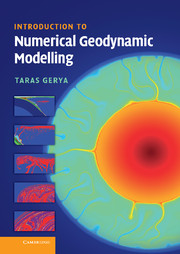
\includegraphics[height=4cm]{images/literature/gerya_book}
b)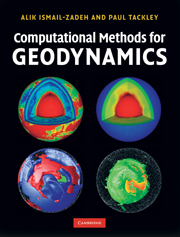
\includegraphics[height=4cm]{images/literature/tackley_book}
c)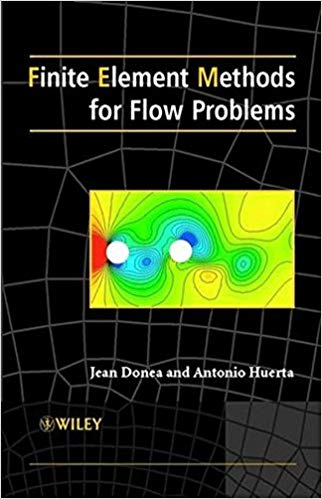
\includegraphics[height=4cm]{images/literature/donea_huerta_book}
d)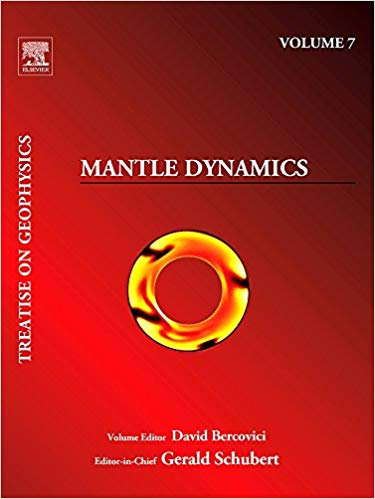
\includegraphics[height=4cm]{images/literature/bercovici_book}
e)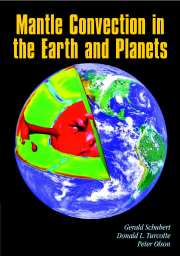
\includegraphics[height=4cm]{images/literature/sto_book}\\
%a) \url{https://doi.org/10.1017/CBO9780511809101}
%b) \url{https://doi.org/10.1017/CBO9780511780820}
%c) \url{https://www.wiley.com/en-us/Finite+Element+Methods+for+Flow+Problems-p-9780471496663}
%d) \url{https://www.elsevier.com/books/treatise-on-geophysics-volume-7/bercovici/978-0-444-51935-1}
\end{center}

%---------------------------------------
\subsection{Installation}

\begin{verbatim}
python3.6 -m pip install --user numpy scipy matplotlib
\end{verbatim}

\newpage
%%%%%%%%%%%%%%%%%%%%%%
\section{The physical equations of Fluid Dynamics}

\begin{center}
\begin{tabular}{lll}
\hline
Symbol & meaning & unit \\
\hline
\hline
$t$ & Time & s \\
$x,y,z$ & Cartesian coordinates & m \\
${\bm v}$ & velocity vector & m$\cdot$ s$^{-1}$\\
$\rho$ & mass density & kg/m$^3$ \\
$\eta$ & dynamic viscosity &  Pa$\cdot$ s \\
$\lambda$ & penalty parameter & Pa$\cdot$ s \\
$T$ & temperature & K \\
${\bm \nabla}$ & gradient operator & m$^{-1}$ \\
${\bm \nabla}\cdot$ & divergence operator & m$^{-1}$ \\
$p$ & pressure & Pa\\
$\dot{\bm \varepsilon}({\bm v})$ & strain rate tensor & s$^{-1}$ \\
$\alpha$ & thermal expansion coefficient & K$^{-1}$ \\
$k$ & thermal conductivity & W/(m $\cdot$ K) \\
$C_p$ & Heat capacity & J/K \\
$H$ & intrinsic specific heat production & W/kg\\
$\beta_T$ & isothermal compressibility & Pa$^{-1}$  \\
${\bm \tau}$ & deviatoric stress tensor & Pa \\
${\bm \sigma}$ & full stress tensor & Pa \\
\hline
\end{tabular}
\end{center}

%------------------------------------------------------------------------
\subsection{The heat transport equation - energy conservation equation}

Let us start from the heat transport equation as shown in Schubert, Turcotte and Olson \cite{scto01}:
\[
\rho C_p \frac{DT}{Dt} - \alpha T \frac{Dp}{Dt} = {\bm \nabla} \cdot k {\bm \nabla} T + \Phi + \rho H  
\]
with $D/Dt$ being the total derivatives so that 
\[
\frac{DT}{Dt} = \frac{\partial T}{\partial t} + {\bm v}\cdot {\bm \nabla}T
\quad\quad
\frac{Dp}{Dt} = \frac{\partial p}{\partial t} + {\bm v}\cdot {\bm \nabla}p
\]
Solving for temperature, this equation is often rewritten as follows:
\begin{mdframed}[backgroundcolor=blue!5]
\[
\rho C_p \frac{DT}{Dt} - {\bm \nabla} \cdot k {\bm \nabla} T =  \alpha T \frac{Dp}{Dt} + \Phi + \rho H  
\]
\end{mdframed}

A note on the shear heating term $\Phi$: In many publications, $\Phi$ 
is given by $\Phi=\tau_{ij}\partial_j u_i={\bm \tau}:{\bm \nabla}{\bm v}$.

\begin{eqnarray}
\Phi 
&=& \tau_{ij}\partial_j u_i \nonumber\\
&=& 2 \eta \dot{\varepsilon}_{ij}^d\partial_j u_i \nonumber\\
&=& 2 \eta \frac{1}{2}\left( \dot{\varepsilon}_{ij}^d\partial_j u_i + \dot{\varepsilon}_{ji}^d\partial_i u_j \right) \nonumber\\
&=& 2 \eta \frac{1}{2}\left( \dot{\varepsilon}_{ij}^d\partial_j u_i + \dot{\varepsilon}_{ij}^d\partial_i u_j \right) \nonumber\\
&=& 2 \eta  \dot{\varepsilon}_{ij}^d  \frac{1}{2}\left(\partial_j u_i + \partial_i u_j \right) \nonumber\\
&=& 2 \eta  \dot{\varepsilon}_{ij}^d   \dot{\varepsilon}_{ij} \nonumber\\
&=& 2 \eta  \dot{\bm \varepsilon}^d :  \dot{\bm \varepsilon} \nonumber\\
&=& 2 \eta  \dot{\bm \varepsilon}^d : \left( \dot{\bm \varepsilon}^d +\frac{1}{3} ({\bm \nabla}\cdot{\bm v}) {\bm 1} \right)\nonumber\\
&=& 2 \eta  \dot{\bm \varepsilon}^d : \dot{\bm \varepsilon}^d 
+ 2 \eta  \dot{\bm \varepsilon}^d : {\bm 1} ({\bm \nabla}\cdot{\bm v}) \nonumber\\ 
&=& 2 \eta  \dot{\bm \varepsilon}^d : \dot{\bm \varepsilon}^d 
\end{eqnarray}
Finally
\[
\Phi = {\bm \tau}:{\bm \nabla}{\bm v} = 2 \eta  \dot{\bm \varepsilon}^d : \dot{\bm \varepsilon}^d
= 2 \eta \left( (\dot{\varepsilon}_{xx}^d)^2 + (\dot{\varepsilon}_{yy}^d)^2 + 2(\dot{\varepsilon}_{xy}^d)^2 \right)
\]

%------------------------------------------------------------------------
\subsection{The momentum conservation equations} 

Because the Prandlt number is virtually zero in Earth science applications the Navier Stokes 
equations reduce to the Stokes equation:
\[
{\bm \nabla}\cdot {\bm \sigma} + \rho {\bm g} = 0
\]
Since 
\[
{\bm \sigma} = -p {\bm 1} + {\bm \tau}
\]
it also writes
\[
-{\bm \nabla}p + {\bm \nabla}\cdot {\bm \tau} + \rho {\bm g} = 0
\]
Using the relationship ${\bm \tau} = 2 \eta \dot{\bm \varepsilon}^d$ we arrive at 
\begin{mdframed}[backgroundcolor=blue!5]
\[
-{\bm \nabla}p + {\bm \nabla}\cdot (2 \eta \dot{\bm \varepsilon}^d ) + \rho {\bm g} = 0
\]
\end{mdframed}

%------------------------------------------------------------------------
\subsection{The mass conservation equations} 

The mass conservation equation is given by
\[
\frac{D\rho}{Dt} + \rho {\bm \nabla}\cdot{\bm v} = 0
\]
or, 
\begin{mdframed}[backgroundcolor=blue!5]
\[
\frac{\partial \rho}{\partial t} + {\bm \nabla}\cdot(\rho {\bm v}) = 0
\]
\end{mdframed}
In the case of an incompressible flow, then $\partial \rho/\partial t=0$ and 
${\bm \nabla}\rho=0$, i.e. $D\rho/Dt=0$ and the remaining equation is simply:
\[
{\bm \nabla}\cdot{\bm v} = 0
\]

\subsection{The equations in ASPECT manual}
The following is lifted off the ASPECT manual.
We focus on the system of equations in a $d=2$- or $d=3$-dimensional
domain $\Omega$ that describes the motion of a highly viscous fluid driven
by differences in the gravitational force due to a density that depends on
the temperature. In the following, we largely follow the exposition of this
material in Schubert, Turcotte and Olson \cite{scto01}.

Specifically, we consider the following set of equations for velocity $\mathbf
u$, pressure $p$ and temperature $T$:
\begin{align}
  \label{eq:stokes-1}
  -\nabla \cdot \left[2\eta \left(\dot\varepsilon(\bm v)
                                  - \frac{1}{3}(\nabla \cdot \bm v)\mathbf 1\right)
                \right] + \nabla p &=
  \rho \bm g
  &
  & \textrm{in $\Omega$},
  \\
  \label{eq:stokes-2}
  \nabla \cdot (\rho \bm v) &= 0
  &
  & \textrm{in $\Omega$},
  \\
  \label{eq:temperature}
  \rho C_p \left(\frac{\partial T}{\partial t} + \bm v\cdot\nabla T\right)
  - \nabla\cdot k\nabla T
  &=
  \rho H
  \notag
  \\
  &\quad
  +
  2\eta
  \left(\dot\varepsilon(\bm v) - \frac{1}{3}(\nabla \cdot \bm v)\mathbf 1\right)
  :
  \left(\dot\varepsilon(\bm v) - \frac{1}{3}(\nabla \cdot \bm v)\mathbf 1\right)
  \\
  &\quad
  +\alpha T \left( \bm v \cdot \nabla p \right)
  \notag
  \\
  &\quad
  &
  & \textrm{in $\Omega$},
  \notag
\end{align}
where $\dot{\bm \varepsilon}(\mathbf u) = \frac{1}{2}(\nabla \mathbf u + \nabla\mathbf
u^T)$ is the symmetric gradient of the velocity (often called the
\textit{strain rate}).%

In this set of equations, \eqref{eq:stokes-1} and \eqref{eq:stokes-2}
represent the compressible Stokes equations in which $\mathbf v=\mathbf
v(\mathbf x,t)$ is the velocity field and $p=p(\mathbf x,t)$ the pressure
field. Both fields depend on space $\mathbf x$ and time $t$. Fluid flow is
driven by the gravity force that acts on the fluid and that is proportional to
both the density of the fluid and the strength of the gravitational pull.

Coupled to this Stokes system is equation \eqref{eq:temperature} for the
temperature field $T=T(\mathbf x,t)$ that contains heat conduction terms as
well as advection with the flow velocity $\mathbf v$. The right hand side
terms of this equation correspond to
\begin{itemize}
\item internal heat production for example due to radioactive decay;
\item friction (shear) heating;
\item adiabatic compression of material;
\end{itemize}

In order to arrive at the set of equations that ASPECT solves, 
we need to 
\begin{itemize}
\item neglect the $\partial p/\partial t$. {\color{red}WHY?}
\item neglect the $\partial \rho / \partial t$ . {\color{red}WHY?}
\end{itemize}
from equations above. 

----------------------------------------

Also, their definition of the shear heating term $\Phi$ is:
\[
\Phi = k_B ({\bm \nabla}\cdot{\bm v})^2 + 2\eta \dot{\bm \varepsilon}^d:\dot{\bm \varepsilon}^d
\]
For many fluids the bulk viscosity $k_B$ is very small and is often taken to be zero, an assumption known
as the Stokes assumption: $k_B=\lambda+2\eta/3=0$. \index{bulk viscosity}
Note that $\eta$ is the dynamic viscosity and $\lambda$ the second viscosity. \index{dynamic viscosity}
\index{second viscosity}
Also, 
\[
{\bm \tau}=2\eta \dot{\bm \varepsilon} + \lambda ({\bm \nabla}\cdot{\bm v}) {\bm 1}
\]
but since $k_B=\lambda+2\eta/3=0$, then $\lambda=-2\eta/3$ so 
\[
{\bm \tau}=2\eta \dot{\bm \varepsilon} -\frac{2}{3}\eta ({\bm \nabla}\cdot{\bm v}) {\bm 1} = 2\eta \dot{\bm \varepsilon}^d
\]







\newpage
%---------------------------------
\subsection{the Boussinesq approximation: an Incompressible flow}

\index{Boussinesq}

[from aspect manual]
The Boussinesq approximation assumes that the density can be
considered constant in all occurrences in the equations with the exception of
the buoyancy term on the right hand side of \eqref{eq:stokes-1}. The primary
result of this assumption is that the continuity equation \eqref{eq:stokes-2}
will now read
\[
{\bm \nabla}\cdot{\bm v} = 0
\]
This implies that the strain rate tensor is deviatoric.
Under the Boussinesq approximation, the equations are much simplified:

\begin{align}
  \label{eq:stokes-1}
  -\nabla \cdot \left[2\eta \dot{\bm \varepsilon}(\bm v)
                \right] + \nabla p &=
  \rho \bm g
  &
  & \textrm{in $\Omega$},
  \\
  \label{eq:stokes-2}
  \nabla \cdot (\rho \bm v) &= 0
  &
  & \textrm{in $\Omega$},
  \\
  \label{eq:temperature}
  \rho_0 C_p \left(\frac{\partial T}{\partial t} + \bm v\cdot\nabla T\right)
  - \nabla\cdot k\nabla T
  &=
  \rho H
  &
  & \textrm{in $\Omega$}
\end{align}
Note that all terms on the rhs of the temperature equations have disappeared, with the exception 
of the source term.


\newpage
%%%%%%%%%%%%%%%%%%%%%%%%%%%%%%%%%%%%%%%%%%%%%%%%%%%%%%%%%%%%%%%%%%%%%%%%%%%%%%%%%%%%%%%%%%55
\subsection{Stokes equation for elastic medium}

What follows is mostly borrowed from Becker \& Kaus lecture notes.

%\begin{tabular}{|l|l|l|}
%\hline
%${\bm u}       $ & displacement vector &   \\
%${\bm \sigma}  $ & full stress tensor  & Pa\\
%${\bm \epsilon}$ & strain tensor       &   \\
%${\bm 1}       $ & unit tensor         &   \\
%${\bm f}       $ & body forces         &   \\
%\hline
%\end{tabular}

The strong form of the PDE that governs force balance in a medium is given by
\[
{\bm \nabla}\cdot{\bm \sigma}  + {\bm f} = {\bm 0}
\]
where ${\bm \sigma}$ is the stress tensor and ${\bm f}$ is a body force.

The stress tensor is related to the strain tensor through the generalised 
Hooke's law:
\begin{equation}
\sigma_{ij}=\sum_{kl}C_{ijkl}\epsilon{kl} \label{eq:one}
\end{equation}
where ${\bm C}$ is the fourth-order elastic tensor.
In the case of an isotropic material, this relationship simplifies to
\begin{equation}
\sigma_{ij}=\lambda \epsilon_{kk} \delta_{ij} + 2\mu \epsilon_{ij}
\quad\quad
or, 
\quad\quad
{\bm \sigma} = \lambda ({\bm \nabla}\cdot{\bm u})  {\bm 1} + 2\mu {\bm \epsilon}   \label{eq:two}
\end{equation}
where $\lambda$ is the Lam\'e parameter and $\mu$ is the shear modulus\footnote{It is also sometimes written $G$}.
The term ${\bm \nabla}\cdot{\bm u}$ is the isotropic dilation.

\index{Lam\'e parameter} \index{shear modulus}

The strain tensor is related to the displacement as follows: \index{strain tensor}
\[
{\bm \epsilon} = \frac{1}{2}({\bm \nabla}{\bm u} + {\bm \nabla}{\bm u}^T)
\]

The incompressibility (bulk modulus), $K$, is defined as $p=-K {\bm \nabla}\cdot{\bm u}$ 
where $p$ is the pressure with \index{bulk modulus}
\begin{eqnarray}
p&=&-\frac{1}{3}Tr({\bm \sigma}) \nonumber\\
 &=& -\frac{1}{3} [ \lambda ({\bm \nabla}\cdot{\bm u}) Tr[{\bm 1}] + 2 \mu Tr[{\bm \epsilon}]] \nonumber\\
 &=& -\frac{1}{3} [ \lambda ({\bm \nabla}\cdot{\bm u})  3  + 2 \mu  ({\bm \nabla}\cdot{\bm u}) ] \nonumber\\
 &=& -[ \lambda  + \frac{2}{3} \mu ]   ({\bm \nabla}\cdot{\bm u})  
\end{eqnarray}
so that $K=\lambda+\frac{2}{3}\mu$.

%or
%\[
%\mu=\frac{3K(1-2\nu)}{2(1+\nu)}
%\]


\paragraph{Remark}: Eq. (\ref{eq:one}) and (\ref{eq:two}) are analogous to the ones that one has to solve
in the context of viscous flow using the penalty method. In this case $\lambda$ is the penalty coefficient, 
${\bm u}$ is the velocity, and $\mu$ is then the dynamic viscosity.

%\begin{center}
%\includegraphics[width=15cm]{images/coeffs}\\
%{\small Homogeneous isotropic linear elastic materials have their elastic properties uniquely determined by any two moduli among these; thus, given any two, any other of the elastic moduli can be calculated according to these formulas.}
%\end{center}

The Lam\'e parameter and the shear modulus are also linked to $\nu$ the poisson ratio, 
and $E$, Young's modulus: \index{Poisson ratio} \index{Young's modulus}
\[
\lambda=\mu\frac{2\nu}{1-2\nu}
=\frac{\nu E}{(1+\nu)(1-2\nu)}
\quad\quad
{\rm with}
\quad\quad
E=2\mu(1+\nu)
\]
The shear modulus, expressed often in GPa, describes the material's response to shear stress.
The poisson ratio describes the response in the direction orthogonal to uniaxial stress.
The Young modulus, expressed in GPa, describes the material's strain response to uniaxial stress in the 
direction of this stress.


%%%%%%%%%%%%%%%%%%%%%%%%%%%%%%%%%%%%%%%%%%%%%%%%%%%%%%%%%%%%%%%%%%55
\newpage
\subsection{The strain rate tensor in all coordinate systems}

The strain rate tensor $\dot{\bm\varepsilon}$ is given by
\begin{equation}
\dot{\bm \varepsilon} = \frac{1}{2}( {\bm \nabla}{\bm v}+ {\bm \nabla}{\bm v}^T) 
\end{equation}

\subsubsection{Cartesian coordinates}
\begin{eqnarray}
\dot\varepsilon_{xx} &=& \frac{\partial u}{\partial x} \\
\dot\varepsilon_{yy} &=& \frac{\partial v}{\partial y} \\
\dot\varepsilon_{zz} &=& \frac{\partial w}{\partial z} \\
\dot\varepsilon_{yx} =
\dot\varepsilon_{xy} &=& \frac{1}{2} \left( \frac{\partial u}{\partial y} + \frac{\partial v}{\partial x}  \right)\\
\dot\varepsilon_{zx} =
\dot\varepsilon_{xz} &=& \frac{1}{2} \left( \frac{\partial u}{\partial z} + \frac{\partial w}{\partial x}  \right)\\
\dot\varepsilon_{zy} =
\dot\varepsilon_{yz} &=& \frac{1}{2} \left( \frac{\partial v}{\partial z} + \frac{\partial w}{\partial y}  \right)
\end{eqnarray}

\subsubsection{Polar coordinates}

\begin{eqnarray}
\dot\varepsilon_{rr} &=& \frac{\partial v_r}{\partial r} \\
\dot\varepsilon_{\theta\theta} &=& \frac{v_r}{r} + \frac{1}{r} \frac{\partial v_\theta}{\partial \theta}  \\
\dot\varepsilon_{\theta r} =
\dot\varepsilon_{r\theta} &=& \frac{1}{2} \left(   \frac{\partial v_\theta}{\partial r} - \frac{v_\theta}{r} 
+\frac{1}{r} \frac{\partial v_r}{\partial \theta}  \right) 
\end{eqnarray}

\subsubsection{Cylindrical coordinates}

http://eml.ou.edu/equation/FLUIDS/STRAIN/STRAIN.HTM

\subsubsection{Sperical coordinates}

\begin{eqnarray}
\dot\varepsilon_{rr} &=& \frac{\partial v_r}{\partial r} \\
\dot\varepsilon_{\theta\theta} &=& \frac{v_r}{r} + \frac{1}{r} \frac{\partial v_\theta}{\partial \theta}  \\
\dot\varepsilon_{\phi\phi} &=& \frac{1}{r \sin\theta} \frac{\partial v_\phi}{\partial \phi} \\
\dot\varepsilon_{\theta r} =
\dot\varepsilon_{r\theta}   &=& \frac{1}{2} \left( r \frac{\partial}{\partial r} (\frac{v_\theta}{r} ) 
+\frac{1}{r} \frac{\partial v_r}{\partial \theta} \right) \\
\dot\varepsilon_{\phi r} =
\dot\varepsilon_{r\phi}      &=&  \frac{1}{2} \left(  \frac{1}{r \sin\theta} \frac{\partial v_r}{\partial \phi} 
+ r \frac{\partial }{\partial r} (\frac{v_\phi}{r}) \right)  \\
\dot\varepsilon_{\phi \theta} =
\dot\varepsilon_{\theta\phi} &=& \frac{1}{2} \left( \frac{\sin \theta}{r} \frac{\partial }{\partial \theta} (\frac{v_\phi}{\sin\theta}) + \frac{1}{r \sin\theta} \frac{\partial v_\theta}{\partial \phi}    \right) 
\end{eqnarray}








\newpage
%------------------------------------------------------------------------------
\section{The Finite Element Method}

\subsection{Numerical integration}
As we will see later, using the Finite Element method to solve problems involves computing integrals which are more often than not too complex to be computed analytically/exactly. We will then need to compute them numerically.

[wiki] In essence, 
the basic problem in numerical integration is to compute an approximate solution to a definite integral
\[
\int_a^b f(x) dx
\]
to a given degree of accuracy.
This problem has been widely studied and we know that 
if $f(x)$ is a smooth function, and the domain of integration is bounded, there are many methods for approximating the integral to the desired precision.

There are several reasons for carrying out numerical integration.
\begin{itemize}
\item The integrand $f(x)$ may be known only at certain points, such as obtained by sampling. Some embedded systems and other computer applications may need numerical integration for this reason.
\item A formula for the integrand may be known, but it may be difficult or impossible to find an antiderivative that is an elementary function. An example of such an integrand is $f(x)=exp(-x^2)$, the antiderivative of which (the error function, times a constant) cannot be written in elementary form.
\item It may be possible to find an antiderivative symbolically, but it may be easier to compute a numerical approximation than to compute the antiderivative. That may be the case if the antiderivative is given as an infinite series or product, or if its evaluation requires a special function that is not available.
\end{itemize}

%-----------------------------
\subsubsection{in 1D - theory}

The simplest method of this type is to let the interpolating function be a constant function (a polynomial of degree zero) that passes through the point $((a+b)/2, f((a+b)/2))$.

This is called the midpoint rule \index{midpoint rule} or rectangle rule. \index{rectangle rule}
\[
\int_a^b f(x)dx \simeq (b-a) f(\frac{a+b}{2})
\]

\improvement[inline]{insert here figure}

The interpolating function may be a straight line (an affine function, i.e. a polynomial of degree 1)
passing through the points $(a, f(a))$ and $(b, f(b))$.

This is called the trapezoidal rule. \index{trapezoidal rule} 
\[
\int_a^b f(x)dx \simeq (b-a) \frac{f(a)+f(b)}{2}
\]

\improvement[inline]{insert here figure}

For either one of these rules, we can make a more accurate approximation by breaking up the interval [a, b] into some number n of subintervals, computing an approximation for each subinterval, then adding up all the results. This is called a composite rule, extended rule, or iterated rule. For example, the composite trapezoidal rule can be stated as

\[
\int_a^b f(x)dx \simeq \frac{b-a}{n} \left( \frac{f(a)}{2}  
+\sum_{k=1}^{n-1} f(a+k\frac{b-a}{n})
   +\frac{f(b)}{2} \right)
\]

where the subintervals have the form $[kh,(k+1)h]$, with $h=(b-a)/n$ and $k=0,1,2,\dots,n-1$.


\begin{center}
a)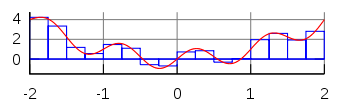
\includegraphics[width=7cm]{images/quadrature/int1}
b)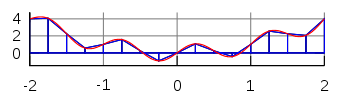
\includegraphics[width=7cm]{images/quadrature/int2}\\
The interval $[-2,2]$ is broken into 16 sub-intervals. The blue lines correspond to the 
approximation of the red curve by means of a) the midpoint rule,  b) the trapezoidal rule.
\end{center}

There are several algorithms for numerical integration (also commonly called 'numerical quadrature', or
simply 'quadrature') \index{quadrature}.
Interpolation with polynomials evaluated at equally spaced points in $[a,b]$
yields the Newton–Cotes formulas, of which the rectangle rule and the trapezoidal rule are examples. \index{Newton-Cotes}
If we allow the intervals between interpolation points to vary, we find another group of quadrature formulas, such as 
the Gauss(ian) quadrature formulas. \index{Gauss quadrature}
A Gaussian quadrature rule is typically more accurate than a Newton–Cotes rule, 
which requires the same number of function evaluations, if the integrand is smooth 
(i.e., if it is sufficiently differentiable).


An $n-$point Gaussian quadrature rule, named after Carl Friedrich Gauss, is a quadrature rule constructed
to yield an exact result for polynomials of degree $2n-1$ or less by a suitable choice of the points $x_i$
and weights $w_i$ for $i=1,\dots,n$.

The domain of integration for such a rule is conventionally taken as $[-1,1]$, so the rule is stated as
\[
\int_{-1}^{+1} f(x) dx = \sum_{i_q=1}^n w_{i_q} f(x_{i_q})
\]
In this formula the $x_{i_q}$ coordinate is 
the $i$-th root of the Legendre polynomial $P_n(x)$. \index{Legendre polynomial}

It is important to note that a Gaussian quadrature will only produce good results if the function $f(x)$
is well approximated by a polynomial function within the range $[-1,1]$.
As a consequence, the method is not, for example, suitable for functions with singularities.

\begin{center}
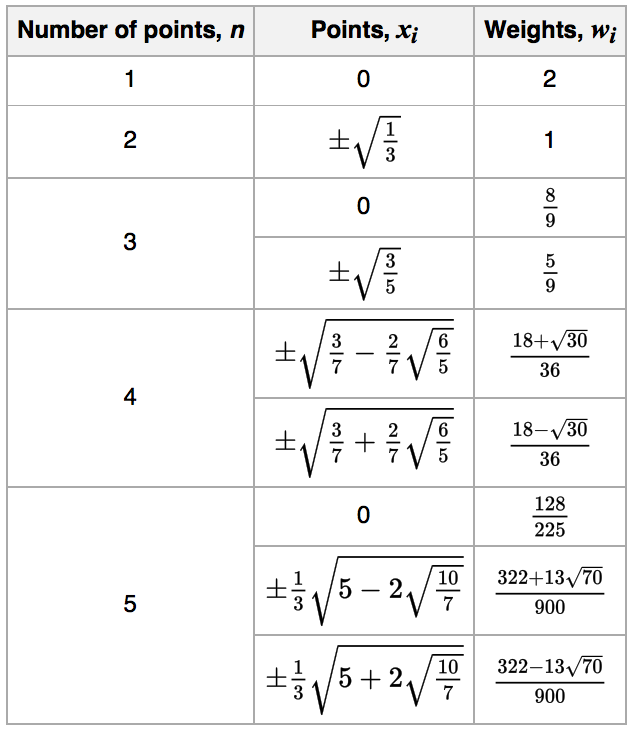
\includegraphics[width=5.cm]{images/quadrature/gq2}\\
Gauss-Legendre points and their weights.
\end{center}

\begin{tabular}{lllll}
\hline
n & $x_{iq}$ & $w_{iq}$ & $x_{iq}$ (approx) & $w_{iq}$ (approx) \\
\hline\hline
1 & 0 & 2 & 0 & 2 \\
\hline
2 & $\pm \sqrt{1/3}$ & 1  & $\pm$0.577350269189626 & 1 \\
\hline
3 & 0 & 8/9 & 0 & 0.888888888888889 \\
  & $\pm\sqrt{3/5}$  & 5/9  & $\pm$0.774596669241483 & 0.555555555555556 \\
\hline
4 & $\pm\sqrt{\frac{3}{7} - \frac{2}{7}\sqrt{6/5}}$  & $\frac{18+\sqrt{30}}{36}$ & $\pm$0.339981043584856 & 0.652145154862546 \\
  & $\pm\sqrt{\frac{3}{7} + \frac{2}{7}\sqrt{6/5}}$  & $\frac{18-\sqrt{30}}{36}$ & $\pm$0.861136311594053 & 0.347854845137454 \\
\hline
5 & 0 & 128/225 & 0 & 0.568888888888889 \\
  & $\pm\frac{1}{3}\sqrt{5-2\sqrt{\frac{10}{7}}}$  & $\frac{322+13\sqrt{70}}{900}$ & $\pm$0.538469310105683 & 0.478628670499366 \\
  & $\pm\frac{1}{3}\sqrt{5+2\sqrt{\frac{10}{7}}}$  & $\frac{322-13\sqrt{70}}{900}$ & $\pm$0.906179845938664 & 0.236926885056189 \\
\hline
6 & ?& ?& $\pm$0.23861 91860 83197 & 0.46791 39345 72691 \\
  & ?& ?& $\pm$0.66120 93864 66265 & 0.36076 15730 48139 \\
  & ?& ?& $\pm$0.93246 95142 03152 & 0.17132 44923 79170 \\
\hline
\end{tabular}



As shown in the above table, it can be shown that the weight values must fulfill the following condition:
\begin{equation}
\sum_{i_q} w_{i_q}=2 \label{gq23}
\end{equation}
and it is worth noting that all quadrature point coordinates are symmetrical around the origin.

Since most quadrature formula are only valid on a specific interval, we now must address the problem 
of their use outside of such intervals. The solution turns out to be quite simple: one 
must carry out a change of variables from the interval $[a,b]$ to $[-1,1]$.

We then consider the reduced coordinate $r\in[-1,1]$ such that 
\[
r=\frac{2}{b-a}(x-a)-1 
\]
This relationship can be reversed such that when $r$ is known, its equivalent coordinate 
$x\in[a,b]$ can be computed:
\[
x=\frac{b-a}{2}(1+r)+a
\]
From this it follows that
\[
dx=\frac{b-a}{2}dr
\]
and then 
\[
\int_a^b f(x) dx  = \frac{b-a}{2} \int_{-1}^{+1} f(r) dr \simeq 
\frac{b-a}{2} \sum_{i_q=1}^n w_{i_q} f(r_{i_q})
\]

%--------------------
\subsubsection{in 1D - examples}

\paragraph{example 1}

Since we know how to carry out any required change of variables, we choose for simplicity 
$a=-1$, $b=+1$.
Let us take for example $f(x)=\pi$. Then we can compute the integral of this function 
over the interval $[a,b]$ exactly:
\[
I=\int_{-1}^{+1} f(x) dx = \pi \int_{-1}^{+1}dx  = 2 \pi
\]
We can now use a Gauss-Legendre formula to compute this same integral:
\[
I_{gq}=\int_{-1}^{+1} f(x) dx 
= \sum_{i_q=1}^{n_q} w_{i_q} f(x_{i_q}) 
= \sum_{i_q=1}^{n_q} w_{i_q} \pi
= \pi \underbrace{\sum_{i_q=1}^{n_q} w_{i_q} }_{=2}
= 2 \pi
\]
where we have used the property of the weight values of Eq.(\ref{gq23}).
Since the actual number of points was never specified, this result is valid for all 
quadrature rules.


\paragraph{example 2}

Let us now take $f(x)=m x+ p$ and repeat the same exercise:
\[
I=\int_{-1}^{+1} f(x) dx = \int_{-1}^{+1} (mx+p) dx  =  [\frac{1}{2} m x^2 + p x ]_{-1}^{+1} =2p
\]
\[
I_{gq}=\int_{-1}^{+1} f(x) dx 
\!= \sum_{i_q=1}^{n_q} w_{i_q} f(x_{i_q}) 
\!= \sum_{i_q=1}^{n_q} w_{i_q} (m x_{i_q} + p)  
\!= m \underbrace{\sum_{i_q=1}^{n_q} w_{i_q} x_{i_q}}_{=0}  + p \underbrace{\sum_{i_q=1}^{n_q} w_{i_q}}_{=2}  = 2p
\]
since the quadrature points are symmetric w.r.t. to zero on the x-axis.
Once again the quadrature is able to compute the exact value of this integral: this makes sense since 
an $n$-point rule exactly integrates a $2n-1$ order polynomial such that a 1 point quadrature exactly 
integrates a first order polynomial like the one above.



\paragraph{example 3}

Let us now take $f(x)=x^2$. We have 
\[
I=\int_{-1}^{+1} f(x) dx = \int_{-1}^{+1} x^2 dx  =  [\frac{1}{3}x^3 ]_{-1}^{+1} =  \frac{2}{3} 
\]
and 
\[
I_{gq}=\int_{-1}^{+1} f(x) dx 
\!= \sum_{i_q=1}^{n_q} w_{i_q} f(x_{i_q}) 
\!= \sum_{i_q=1}^{n_q} w_{i_q} x_{i_q}^2 
\]

\begin{itemize}
\item $n_q=1$: $x_{iq}^{(1)}=0$, $w_{i_q}=2$. $I_{gq}=0$
\item $n_q=2$: $x_{q}^{(1)}=-1/\sqrt{3}$, $x_{q}^{(2)}=1/\sqrt{3}$, $w_{q}^{(1)}=w_{q}^{(2)}=1$. $I_{gq}=\frac{2}{3}$
\item It also works $\forall n_q>2$ !
\end{itemize}

%-----------------------------
\subsubsection{in 2D/3D - theory}


Let us now turn to a two-dimensional integral of the form
\[
I=\int_{-1}^{+1} \int_{-1}^{+1} f(x,y) dx dy
\]
The equivalent Gaussian quadrature writes:
\[
I_{gq}
\simeq \sum_{i_q=1}^{n_q}\sum_{j_q}^{n_q} f(x_{i_q},y_{j_q}) w_{i_q} w_{j_q}
\]

%----------------------------------------
\subsubsection{quadrature on triangles}

Quadrature rules for triangles can be found in Dunavant, 1985 \cite{duna85}.
The following ones are identical to those in the {\sl ip\_triangle.m} 
file of the MILAMIN code \cite{daks08}.

{\small
\[
\begin{array}{ccccccc}
\hline
&r_q & s_q & w_q \\ 
\hline\hline
iq=1& 1/3 & 1/3 & 1/2\\
\hline
iq=1 & 1/6 & 1/6 & 1/6 \\
iq=2 & 2/3 & 1/6 & 1/6 \\
iq=3 & 1/6 & 2/3 & 1/6 \\
\hline
iq=1&1/3 & 1/3 & -27/96\\
iq=2&0.6 & 0.2 &  25/96\\
iq=3&0.2 & 0.6 &  25/96\\
iq=4&0.2 & 0.2 &  25/96\\
\hline
iq=1& 1-2g_1 & g_1 & w_1/2  &  0.108103018168070 & 0.44594849091596  &   \\
iq=2& g_1 & 1-2g_1 & w_1/2  &  0.445948490915965 & 0.108103018168070 &   \\
iq=3& g_1 & g_1    & w_1/2  &  0.445948490915965 & 0.445948490915965 &   \\
iq=4& 1-2g_2 & g_2 & w_2/2  &  0.816847572980459 & 0.091576213509771 &   \\
iq=5& g_2 & 1-2g_2 & w_2/2  &  0.091576213509771 & 0.816847572980459 &   \\
iq=6& g_2 & g_2    & w_2/2  &  0.091576213509771 & 0.091576213509771 &   \\
\hline
iq=1&&&&0.091576213509771 &  0.091576213509771    &    0.109951743655322/2.0 \\ 
iq=2&&&&0.816847572980459 &  0.091576213509771    &    0.109951743655322/2.0 \\
iq=3&&&&0.091576213509771 &  0.816847572980459    &    0.109951743655322/2.0 \\
iq=4&&&&0.445948490915965 &  0.445948490915965    &    0.223381589678011/2.0 \\
iq=5&&&&0.108103018168070 &  0.445948490915965    &    0.223381589678011/2.0 \\
iq=6&&&&0.445948490915965 &  0.108103018168070    &    0.223381589678011/2.0 \\
\hline
iq=1 &&&&0.1012865073235 &  0.1012865073235  &     0.0629695902724 \\
iq=2 &&&&0.7974269853531 &  0.1012865073235  &     0.0629695902724 \\
iq=3 &&&&0.1012865073235 &  0.7974269853531  &     0.0629695902724 \\
iq=4 &&&&0.4701420641051 &  0.0597158717898  &     0.0661970763942 \\
iq=5 &&&&0.4701420641051 &  0.4701420641051  &     0.0661970763942 \\
iq=6 &&&&0.0597158717898 &  0.4701420641051  &     0.0661970763942 \\
iq=7 &&&&0.3333333333333 &  0.3333333333333  &     0.1125000000000 \\
\hline
iq=1&&&& 5.01426509658179E-01&  2.49286745170910E-01 &   5.83931378631895E-02 \\ 
iq=2&&&& 2.49286745170910E-01&  5.01426509658179E-01 &   5.83931378631895E-02 \\ 
iq=3&&&& 2.49286745170910E-01&  2.49286745170910E-01 &   5.83931378631895E-02 \\ 
iq=4&&&& 8.73821971016996E-01&  6.30890144915020E-02 &   2.54224531851035E-02 \\ 
iq=5&&&& 6.30890144915020E-02&  8.73821971016996E-01 &   2.54224531851035E-02 \\ 
iq=6&&&& 6.30890144915020E-02&  6.30890144915020E-02 &   2.54224531851035E-02 \\ 
iq=7&&&& 5.31450498448170E-02&  3.10352451033784E-01 &   4.14255378091870E-02 \\ 
iq=8&&&& 6.36502499121399E-01&  5.31450498448170E-02 &   4.14255378091870E-02 \\ 
iq=9&&&& 3.10352451033784E-01&  6.36502499121399E-01 &   4.14255378091870E-02 \\ 
iq=10&&&& 5.31450498448170E-02&  6.36502499121399E-01 &   4.14255378091870E-02 \\ 
iq=11&&&& 6.36502499121399E-01&  3.10352451033784E-01 &   4.14255378091870E-02 \\ 
iq=12&&&& 3.10352451033784E-01&  5.31450498448170E-02 &   4.14255378091870E-02 \\ 
\hline
\end{array}
\]
}

where
\[ 
g_1 = \left(8-\sqrt{10} + \sqrt{38-44\sqrt{2/5}}\right)/18
\qquad
g_2 = \left(8-\sqrt{10} - \sqrt{38-44\sqrt{2/5}}\right)/18
\]
\[
w_1 = \left(620+\sqrt{213125-53320\sqrt{10}}\right)/3720
\qquad
w_2 = \left(620-\sqrt{213125-53320\sqrt{10}}\right)/3720
\]


      


%----------------------------------------
\subsubsection{quadrature on tetrahedra}

\begin{remark}
In what follows the coefficients in the tables are not the reduced coordinates
of the quadratue points but the coefficients corresponding to the 4 nodes.
\end{remark}

Quadrature rules on tetrahedra take the form:
\[
\int\int\int_{el} f(x,y,z) dxdydz = V_{el} \sum_{iq=1}^{nqel} w_{iq} f(\xi^{iq}_1,\xi^{iq}_2,\xi^{iq}_3,\xi^{iq}_4) 
\]
or, that is to say:
\[
\int\int\int_{el} f(x,y,z) dxdydz = \sum_{iq=1}^{nqel} (w_{iq}V_{el}) f(\xi^{iq}_1,\xi^{iq}_2,\xi^{iq}_3,\xi^{iq}_4) 
\]
with in our case $V_{el}=1/6$.

In the literature it can be found that a one point quadrature is characterised by 
\[
w_{iq}=1 \quad\quad\quad \xi^{iq}_1=\xi^{iq}_2=\xi^{iq}_3=\xi^{iq}_4=0.25
\]
i.e, the coordinates of the single point are given by:
\[
x_{iq}=\sum_{i=1}^4 \xi_i^{iq} x_i = \frac{1}{4} (x_1+x_2+x_3+x_4)
\]
Same for $y$ and $z$ coordinates. 

A four-point quadrature rule is characterised by $w_{iq}=V_el*0.25=1/24\simeq 04166666666666667$ and 

\begin{tabular}{lcccc}
 & $\xi_1$ & $\xi_2$ & $\xi_3$ & $\xi_4$ \\
iq=1 & 0.585410196624969 & 0.138196601125011 & 0.138196601125011 & 0.138196601125011 \\
iq=2 & 0.138196601125011 & 0.585410196624969 & 0.138196601125011 & 0.138196601125011 \\
iq=3 & 0.138196601125011 & 0.138196601125011 & 0.585410196624969 & 0.138196601125011 \\
iq=4 & 0.138196601125011 & 0.138196601125011 & 0.138196601125011 & 0.585410196624969 \\
\end{tabular}

We then have:
\[
r_{iq}=\sum_{i=1}^4 \xi_i^{iq} x_i 
= (\xi_1^{iq},\xi_2^{iq},\xi_3^{iq},\xi_4^{iq})\cdot(r_1,r_2,r_3,r_4) 
= (\xi_1^{iq},\xi_2^{iq},\xi_3^{iq},\xi_4^{iq})\cdot(0,1,0,0) 
= \xi_2^{iq}
\]
\[
s_{iq}=\sum_{i=1}^4 \xi_i^{iq} y_i 
= (\xi_1^{iq},\xi_2^{iq},\xi_3^{iq},\xi_4^{iq})\cdot(s_1,s_2,s_3,s_4) 
= (\xi_1^{iq},\xi_2^{iq},\xi_3^{iq},\xi_4^{iq})\cdot(0,0,1,0) 
= \xi_3^{iq}
\]
\[
t_{iq}=\sum_{i=1}^4 \xi_i^{iq} z_i 
= (\xi_1^{iq},\xi_2^{iq},\xi_3^{iq},\xi_4^{iq})\cdot(t_1,t_2,t_3,t_4) 
= (\xi_1^{iq},\xi_2^{iq},\xi_3^{iq},\xi_4^{iq})\cdot(0,0,0,1) 
= \xi_4^{iq}
\]
Finally:

\[
\begin{array}{ccccc}
     & r_q & s_q & t_q  & w_q \\
iq=1 & 0.138196601125011 & 0.138196601125011 & 0.138196601125011 & 0.04166666666666667\\
iq=2 & 0.585410196624969 & 0.138196601125011 & 0.138196601125011 & 0.04166666666666667\\
iq=3 & 0.138196601125011 & 0.585410196624969 & 0.138196601125011 & 0.04166666666666667\\
iq=4 & 0.138196601125011 & 0.138196601125011 & 0.585410196624969 & 0.04166666666666667\\
\end{array}
\]






\subsection{The mesh}

\subsection{A bit of FE terminology}

We introduce here some terminology for efficient element descriptions \cite{grsa}:
\begin{itemize}
\item For triangles/tetrahedra, the designation 
$P_m \times P_n$ \index{$P_m \times P_n$}
means that each component of the velocity
is approximated by continuous piecewise \index{piecewise} complete Polynomials of degree $m$ and
pressure by continuous piecewise complete Polynomials of degree  $n$.
For example $P_2 \times P_1$ means 
\[
u \sim a_1 + a_2 x + a_3 y + a_4 xy + a_5 x^2 + a_6 y^2
\]
with similar approximations for $v$, and 
\[
p \sim b_1 + b_2x + b_3 y
\]
Both velocity and pressure are continuous across element boundaries, 
and each triangular element contains 6 velocity nodes and three pressure nodes.

\item For the same families, \index{$P_m \times P_{-n}$} 
$P_m \times P_{-n}$
is as above, except that pressure is approximated via 
piecewise {\sl discontinuous} polynomials of degree $n$. For instance, $P_2 \times P_{-1}$ is the same 
as $P_2P_1$ except that pressure is now an independent linear function in each element and therefore 
discontinuous at element boundaries.

\item For quadrilaterals/hexahedra, the designation 
\index{$Q_m \times Q_n$}  $Q_m \times Q_n$
means that each component of the velocity
is approximated by a continuous piecewise polynomial of degree $m$ {\sl in each direction} on the quadrilateral
and likewise for pressure, except that the polynomial is of degree $n$.
For instance,  $Q_2 \times Q_1$ \index{$Q_2 \times Q_1$} means
\[
u \sim a_1 + a_2 x + a_3 y + a_4 xy + a_5 x^2 + a_6 y^2 + a_7 x^2y + a_8 xy^2 + a_9 x^2y^2
\]
and 
\[
p \sim b_1 + b_2x + b_3 y + b_4 xy
\]
\item For these same families, $Q_m \times Q_{-n}$ is as above, except that the pressure approximation 
is not continuous at element boundaries. \index{$Q_m \times Q_{-n}$}

\item Again for the same families, \index{$Q_m \times P_{-n}$} $Q_m \times P_{-n}$
 indicates the same velocity approximation 
with a pressure approximation that is a discontinuous complete piecewise polynomial of degree $n$
(not of degree $n$ in each direction !)

\item The designation $P_m^+$ or $Q_m^+$ means that some sort of bubble function \index{bubble function}
was added to the polynomial approximation for the velocity. You may also find the term 'enriched element'
in the literature.

\item Finally, for $n=0$, we have piecewise-constant pressure, and we omit the minus sign for simplicity.
\end{itemize}

Another point which needs to be clarified is the use of so-called 'conforming elements' 
(or 'non-conforming elements'). \index{conforming element} \index{non-conforming element}
Following again \cite{grsa}, conforming velocity elements are those for which the basis functions for a subset 
of $H^1$ for the continuous problem (the first derivatives and their squares are integrable in $\Omega$).
For instance, the rotated $Q_1 \times P_0$ element of Rannacher and Turek (see section \ref{ncq1p0}) is such that 
the velocity is discontinous across element edges, so that the derivative does not exist there. Another
typical example of non-conforming element is the Crouzeix-Raviart element \cite{crra73}.

 




\subsection{Elements and basis functions in 1D}

\subsection{Elements and basis functions in 2D}
Let us for a moment consider a single quadrilateral element in the $xy$-plane, 
as shown on the following figure:
\begin{center}
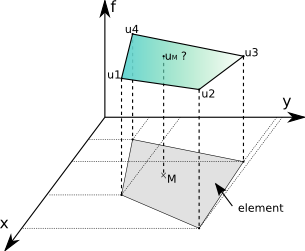
\includegraphics[width=5.8cm]{images/shape.png}
\end{center}
Let us assume that we know the values of a given field $u$ at the vertices.
For a given point $M$ inside the element in the plane, what is the value of the 
field $u$ at this point?
It makes sense to postulate that $u_M=u(x_M,y_M)$ will be given  by 
\[
u_M= \phi(u_1,u_2,u_3,u_4,x_M,y_M) 
\]
where $\phi$ is a function to be determined. Although $\phi$ is not unique, we can 
decide to express the value $u_M$ as a weighed sum of the values at the vertices $u_i$.
One option could be to assign all four vertices the same weight, say $1/4$ so that 
$u_M=(u_1+u_2+u_3+u_4)/4$, i.e. $u_M$ is simply given by the arithmetic mean 
of the vertices values. This approach suffers from a major drawback as it does
not use the location of point $M$ inside the element. For instance, when 
$(x_M,y_M) \rightarrow (x_2,y_2)$ we expect $u_M \rightarrow u_2$.

In light of this, we could now assume that the weights would depend on the position 
of $M$ in a continuous fashion:
\[
u(x_M,y_M) = \sum_{i=1}^4 N_i(x_M,y_M)\;  u_i
\]
where the $N_i$ are continous ("well behaved") functions which have the property:
\[
N_i(x_j,y_j)=\delta_{ij}
\]
or, in other words: 
\begin{eqnarray}
N_3(x_1,y_1) &=& 0 \\
N_3(x_2,y_2) &=& 0 \\
N_3(x_3,y_3) &=& 1 \\
N_3(x_4,y_4) &=& 0 
\end{eqnarray}
The functions $N_i$ are commonly called basis functions. \index{basis functions}

Omitting the $M$ subscripts for any point inside the element, the velocity components $u$
and $v$ are given by:
\[
u(x,y) = \sum_{i=1}^4 N_i(x,y)\;  u_i
\]
\[
v(x,y) = \sum_{i=1}^4 N_i(x,y)\;  v_i
\]
Rather interestingly, one can now easily compute velocity gradients (and therefore the 
strain rate tensor) since we have assumed the basis functions to be "well behaved" 
(in this case differentiable):
\begin{eqnarray}
\dot{\epsilon}_{xx}(x,y) &=& \frac{\partial u}{\partial x} = \sum_{i=1}^4 \frac{\partial N_i}{\partial x}\;  u_i \\
\dot{\epsilon}_{yy}(x,y) &=& \frac{\partial v}{\partial y} = \sum_{i=1}^4 \frac{\partial N_i}{\partial y}\;  v_i \\
\dot{\epsilon}_{xy}(x,y) &=& \frac{1}{2}\frac{\partial u}{\partial y} 
+ \frac{1}{2}\frac{\partial v}{\partial x} 
= \frac{1}{2}\sum_{i=1}^4 \frac{\partial N_i}{\partial y}\;  u_i
+ \frac{1}{2}\sum_{i=1}^4 \frac{\partial N_i}{\partial x}\;  v_i
\end{eqnarray}
How we actually obtain the exact form of the basis functions is explained in the coming section.


%%%%%%%%%%%%%%%%%%%%%%%%%%%%%%%%%%%%5
\subsubsection{The $Q_1$ space}



\begin{center}
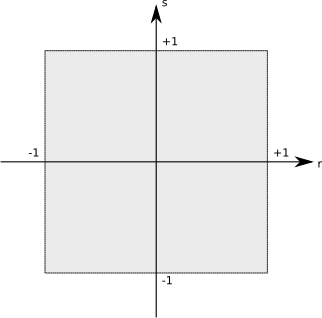
\includegraphics[height=3.5cm]{images/element_rs.png}
\end{center}

\begin{eqnarray}
N_1(r,s)&=&0.25(1-r)(1-s) \nonumber\\
N_2(r,s)&=&0.25(1+r)(1-s) \nonumber\\
N_3(r,s)&=&0.25(1+r)(1+s) \nonumber\\
N_4(r,s)&=&0.25(1-r)(1+s) \nonumber
\end{eqnarray}

\begin{eqnarray}
\frac{\partial N_1}{\partial r}(r,s)&=& - 0.25(1-s) \nonumber\\
\frac{\partial N_2}{\partial r}(r,s)&=& + 0.25(1-s) \nonumber\\
\frac{\partial N_3}{\partial r}(r,s)&=& + 0.25(1+s) \nonumber\\
\frac{\partial N_4}{\partial r}(r,s)&=& - 0.25(1+s) \nonumber
\end{eqnarray}

\begin{eqnarray}
\frac{\partial N_1}{\partial s}(r,s)&=& - 0.25(1-r) \nonumber\\
\frac{\partial N_2}{\partial s}(r,s)&=& - 0.25(1+r) \nonumber\\
\frac{\partial N_3}{\partial s}(r,s)&=& + 0.25(1+r) \nonumber\\
\frac{\partial N_4}{\partial s}(r,s)&=& + 0.25(1-r) \nonumber
\end{eqnarray}




\subsection{The penalty approach}
\label{sec_penalty}

\index{penalty formulation}

In order to impose the incompressibility constraint, two widely used procedures are available, namely the 
Lagrange multiplier method and the penalty method \cite{bathe82,hugh}. The latter is implemented in {\sc elefant}, which allows for the elimination of the pressure variable from the momentum equation (resulting in a reduction of the matrix size).%, based on a relaxation of the incompressibility constraint. 

Mathematical details on the origin and validity of the penalty approach applied to the Stokes problem can for instance be found in  \cite{cuss86}, \cite{redd82} or \cite{gunz89}.

The penalty formulation of the mass conservation equation is based on a relaxation of the incompressibility constraint and writes 
\begin{equation}
{\vec \nabla}\cdot {\vec \upnu} + \frac{p}{\lambda} = 0 \label{penal}
\end{equation}
where $\lambda$ is the penalty parameter, that can be interpreted (and has the same dimension) as a bulk viscosity. It is 
equivalent to say that the material is weakly compressible. It can be shown that if one chooses $\lambda$ to be a 
sufficiently large number, the continuity equation $ {\vec \nabla}\cdot {\vec \upnu} = 0$ will be approximately satisfied in the finite element solution. The value of $\lambda$ is often recommended to be 6 to 7 orders of magnitude larger than the shear viscosity \cite{dohu03,hulb79}.

%Note that Eq. (\ref{penal}) does not form the basis of the penalty method (as often implied) for the Stokes equation but is a consequence of minimising a modified functional of the problem under certain assumptions \cite{redd82}. 

Equation (\ref{penal}) can be used to eliminate the pressure in Eq. (\ref{mce2}) so that the mass and momentum conservation equations fuse to become :
\begin{equation}
{\vec \nabla}\cdot ( 2 \eta \dot\varepsilon({\vec \upnu})) 
+ \lambda {\vec \nabla} ({\vec \nabla }\cdot {\vec \upnu}) = \rho {\bm g} = 0 \label{peneq}
\end{equation}

\cite{mahu78} have established the equivalence for incompressible problems between the reduced integration
of the penalty term and a mixed Finite Element approach if the pressure nodes coincide with the integration points of the reduced rule.

In the end, the elimination of the pressure unknown in the Stokes equations
replaces the original saddle-point Stokes problem \cite{begl05} by an elliptical problem, 
which leads to a symmetric positive definite (SPD) FEM matrix. 
%Such systems always admit a square root triangular matrix (the Cholesky factor, L) and can be solved, once L has been computed (Cholesky factorization), by 2 triangular matrix solves (upper and lower back-substitutions). 
This is the major benefit of the penalized approach 
over the full indefinite solver with the velocity-pressure variables. Indeed, the SPD character of the matrix lends itself 
to efficient solving stragegies and is less memory-demanding since it is sufficient to store only the upper half of the matrix including the diagonal
\cite{gova}
.
\improvement{list codes which use this approach}


The stress tensor ${\bm \sigma}$ is symmetric ({\it i.e.} $\sigma_{ij}=\sigma_{ji}$). For simplicity
I will now focus on a Stokes flow in two dimensions. 

Since the penalty formulation is only valid for incompressible flows, then 
$\dot{\bm \epsilon}=\dot{\bm \epsilon}^d$ so that the $d$ superscript is ommitted in what follows.
The stress tensor can also be cast in vector format:
\begin{eqnarray}
\left(
\begin{array}{c}
\sigma_{xx}\\
\sigma_{yy}\\
\sigma_{xy}\\
\end{array}
\right)
&=&
\left(
\begin{array}{c}
-p \\
-p\\
0
\end{array}
\right)
+2 \eta
\left(
\begin{array}{c}
\dot{\epsilon}_{xx}\\
\dot{\epsilon}_{yy}\\
\dot{\epsilon}_{xy}\\
\end{array}
\right)
\nonumber\\
&=&
\lambda
\left(
\begin{array}{c}
\dot{\epsilon}_{xx} + \dot{\epsilon}_{yy}\\
\dot{\epsilon}_{xx} + \dot{\epsilon}_{yy}\\
0
\end{array}
\right)
+2 \eta
\left(
\begin{array}{c}
\dot{\epsilon}_{xx}\\
\dot{\epsilon}_{yy}\\
\dot{\epsilon}_{xy}\\
\end{array}
\right)\nonumber\\
&=&
\left[
\lambda
\underbrace{
\left(
\begin{array}{ccc}
1 & 1 & 0\\
1 & 1 & 0\\
0 & 0 & 0\\
\end{array}
\right)}_{\bm K}
+ \eta
\underbrace{
\left(
\begin{array}{ccc}
2 & 0 & 0 \\
0 & 2 & 0 \\
0 & 0 & 1 \\
\end{array}
\right)
}_{\bm C}
\right]
\cdot
\left(
\begin{array}{c}
\frac{\partial u}{\partial x} \\ \\
\frac{\partial v}{\partial y} \\ \\
\frac{\partial u}{\partial y} + \frac{\partial v}{\partial x} \\
\end{array}
\right) \nonumber
\end{eqnarray}


Remember that
\[
\frac{\partial u}{\partial x} = \sum_{i=1}^4 \frac{\partial N_i}{\partial x}\;  u_i 
\quad\quad
\frac{\partial v}{\partial y} = \sum_{i=1}^4 \frac{\partial N_i}{\partial y}\;  v_i 
\]

\[
\frac{\partial u}{\partial y} 
+\frac{\partial v}{\partial x} 
= \sum_{i=1}^4 \frac{\partial N_i}{\partial y}\;  u_i
+ \sum_{i=1}^4 \frac{\partial N_i}{\partial x}\;  v_i
\]

so that
\[
\left(
\begin{array}{c}
\frac{\partial u}{\partial x} \\ \\
\frac{\partial v}{\partial y} \\ \\
\frac{\partial u}{\partial y} + \frac{\partial v}{\partial x} \\
\end{array}
\right)
=
\underbrace{
\left(
\begin{array}{cccccccc}
\frac{\partial N_1}{\partial x} & 0 & \frac{\partial N_2}{\partial x} & 0 & \frac{\partial N_3}{\partial x} & 0 & \frac{\partial N_4}{\partial x} & 0 \\  \\
0 & \frac{\partial N_1}{\partial y} & 0 & \frac{\partial N_2}{\partial y} & 0 & \frac{\partial N_3}{\partial y} & 0 & \frac{\partial N_4}{\partial y}  \\ \\
\frac{\partial N_1}{\partial y} &  \frac{\partial N_1}{\partial x} &  \frac{\partial N_2}{\partial y} &  \frac{\partial N_2}{\partial x} & 
\frac{\partial N_3}{\partial y} &  \frac{\partial N_3}{\partial x} &  \frac{\partial N_3}{\partial y} &  \frac{\partial N_4}{\partial x}  
\end{array}
\right)
}_{\bm B}
\cdot
\underbrace{
\left(
\begin{array}{c}
u1 \\ v1 \\ u2 \\ v2 \\ u3 \\ v3 \\ u4 \\ v4
\end{array}
\right)
}_{\bm V}
\]
Finally,
\[
\vec{\sigma}=
\left(
\begin{array}{c}
\sigma_{xx}\\
\sigma_{yy}\\
\sigma_{xy}\\
\end{array}
\right)
=
(\lambda {\bm K} +  \eta {\bm C} )\cdot {\bm B} \cdot {\bm V}
\]

\index{weak form}
We will now establish the weak form of the momentum conservation equation. 
We start again from 
\[
{\vec \nabla}\cdot {\bm \sigma} + {\vec b} = {\vec 0} 
\]
For the $N_i$'s 'regular enough', we can write:
\[
\int_{\Omega_e} N_i {\vec \nabla}\cdot {\bm \sigma} d\Omega + \int_{\Omega_e} N_i  {\bm b} d\Omega =0
\]
We can integrate by parts and drop the surface term\footnote{We will come back to this at a later stage}:
\[
\int_{\Omega_e} {\vec \nabla } N_i \cdot {\bm \sigma} d\Omega = \int_{\Omega_e} N_i  {\bm b} d\Omega 
\]
or, 
\[
\int_{\Omega_e} 
\left(
\begin{array}{ccc}
\frac{\partial N_i}{\partial x} & 0 & \frac{\partial N_i}{\partial y} \\  \\
0 & \frac{\partial N_i}{\partial y} &  \frac{\partial N_i}{\partial x}  
\end{array}
\right)
\cdot
\left(
\begin{array}{c}
\sigma_{xx}\\
\sigma_{yy}\\
\sigma_{xy}\\
\end{array}
\right)
d\Omega = \int_{\Omega_e} N_i {\bm b} d\Omega 
\]
Let $i=1,2,3,4$ and stack the resulting four equations on top of one another. 
\begin{eqnarray}
\int_{\Omega_e} 
\left(
\begin{array}{ccc}
\frac{\partial N_1}{\partial x} & 0 & \frac{\partial N_1}{\partial y} \\  \\
0 & \frac{\partial N_1}{\partial y} &  \frac{\partial N_1}{\partial x}  
\end{array}
\right)
\cdot
\left(
\begin{array}{c}
\sigma_{xx}\\
\sigma_{yy}\\
\sigma_{xy}\\
\end{array}
\right)
d\Omega &=& \int_{\Omega_e} N_1 
\left(
\begin{array}{c}
b_x \\ b_y
\end{array}
\right)
 d\Omega \\
\int_{\Omega_e} 
\left(
\begin{array}{ccc}
\frac{\partial N_2}{\partial x} & 0 & \frac{\partial N_2}{\partial y} \\  \\
0 & \frac{\partial N_2}{\partial y} &  \frac{\partial N_2}{\partial x}  
\end{array}
\right)
\cdot
\left(
\begin{array}{c}
\sigma_{xx}\\
\sigma_{yy}\\
\sigma_{xy}\\
\end{array}
\right)
d\Omega &=& \int_{\Omega_e} N_i 
\left(
\begin{array}{c}
b_x \\ b_y
\end{array}
\right)
d\Omega \\
\int_{\Omega_e} 
\left(
\begin{array}{ccc}
\frac{\partial N_3}{\partial x} & 0 & \frac{\partial N_3}{\partial y} \\  \\
0 & \frac{\partial N_3}{\partial y} &  \frac{\partial N_3}{\partial x}  
\end{array}
\right)
\cdot
\left(
\begin{array}{c}
\sigma_{xx}\\
\sigma_{yy}\\
\sigma_{xy}\\
\end{array}
\right)
d\Omega &=& \int_{\Omega_e} N_3 
\left(
\begin{array}{c}
b_x \\ b_y
\end{array}
\right)
d\Omega \\
\int_{\Omega_e} 
\left(
\begin{array}{ccc}
\frac{\partial N_4}{\partial x} & 0 & \frac{\partial N_4}{\partial y} \\  \\
0 & \frac{\partial N_4}{\partial y} &  \frac{\partial N_4}{\partial x}  
\end{array}
\right)
\cdot
\left(
\begin{array}{c}
\sigma_{xx}\\
\sigma_{yy}\\
\sigma_{xy}\\
\end{array}
\right)
d\Omega &=& \int_{\Omega_e} N_4 
\left(
\begin{array}{c}
b_x \\ b_y
\end{array}
\right)
d\Omega 
\end{eqnarray}
We easily recognize ${\bm B}^T$ inside the integrals!
Let us define 
\[
{\bm N}_b^T=(N_1 b_x , N_1 b_y, ... N_4 b_x, N_4 b_y)
\]
then we can write
\[
\int_{\Omega_e} {\bm B}^T \cdot 
\left(
\begin{array}{c}
\sigma_{xx}\\
\sigma_{yy}\\
\sigma_{xy}\\
\end{array}
\right)
d\Omega
=
\int_{\Omega_e} {\bm N}_b d\Omega 
\]
and finally:
\[
\int_{\Omega_e} {\bm B}^T \cdot [ \lambda {\bm K} + \eta {\bm C} ] \cdot {\bm B} \cdot {\bm V} d\Omega
=
\int_{\Omega_e} {\bm N}_b d\Omega 
\]
Since $V$ contains the velocities at the corners, it does not depend on the $x$ or $y$ coordinates
so it can be taking outside of the integral:
\[
\underbrace{
\left(\int_{\Omega_e} {\bm B}^T \cdot [ \lambda {\bm K} + \eta {\bm C} ] \cdot {\bm B} d\Omega \right) 
}_{A_{el}(8 \times 8)}
\cdot 
\underbrace{
{\bm V}
}_{(8x1)}
=
\underbrace{
\int_{\Omega_e} {\bm N}_b d\Omega 
}_{B_{el} (8\times 1)}
\]
or, 
\[
\left[
\underbrace{
\left(\int_{\Omega_e} \lambda {\bm B}^T \cdot {\bm K} \cdot {\bm B} d\Omega \right) 
}_{A_{el}^\lambda(8 \times 8)}
+
\underbrace{
\left(\int_{\Omega_e}  \eta {\bm B}^T \cdot {\bm C}  \cdot {\bm B} d\Omega \right) 
}_{A_{el}^\eta(8 \times 8)}
\right]
\cdot 
\underbrace{
{\bm V}
}_{(8x1)}
=
\underbrace{
\int_{\Omega_e} {\bm N}_b d\Omega 
}_{B_{el} (8\times 1)}
\]

INTEGRATION - MAPPING 

reduced integration \cite{hulb79}

\begin{enumerate}

\item partition domain $\Omega$ into elements $\Omega_e$, $e=1, ... n_{el}$.


\item loop over elements and for each element compute ${\bm A}_{el}$, ${\bm B}_{el}$ \\
\begin{center}
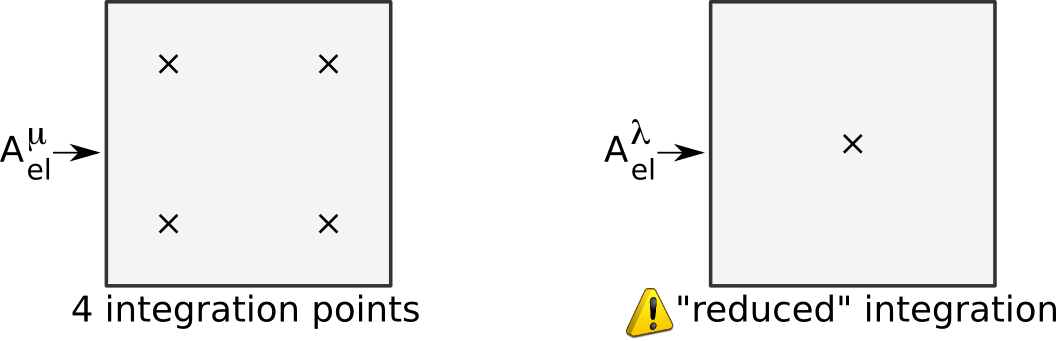
\includegraphics[width=5.5cm]{images/integration.png}
\end{center}

%
\includegraphics[width=0.5cm]{images/warning.png}
%4-point integration for ${\bm A}_{el}^\mu$, 1-point integration for ${\bm A}_{el}^\lambda$


\item a node belongs to several elements\\
      $\rightarrow$ need to assemble ${\bm A}_{el}$ and ${\bm B}_{el}$ in ${\bm A}$, ${\bm B}$

\item apply boundary conditions

\item solve system: ${\bm x}= {\bm A}^{-1} \cdot {\bm B}$
\item visualise/analyse ${\bm x}$
\end{enumerate}



%\subsection{Solving procedures}

%\subsubsection{the whole matrix at once}

%\subsubsection{the pressure Schur complement appraoch}



\newpage
%------------------------------------------------------------------------------
\section{Additional techniques}

\subsection{The method of manufactured solutions}

\subsection{Assigning values to quadrature points}

As we have seen in Section \ref{XXX}, the building of the elemental matrix and rhs
requires (at least) to assign a density and viscosity value to each quadrature point inside
the element. Depending on the type of modelling, this task can prove more complex than 
one might expect and have large consequences on the solution accuracy.

Here are several options:

\begin{itemize}
\item The simplest way (which is often used for benchmarks) consists in computing the 'real'
coordinates $(x_q,y_q,z_q)$ of a given quadrature point based on its reduced coordinates 
$(r_q,s_q,t_q)$, and passing these coordinates to a function which returns density and/or viscosity
at this location. For instance, for the Stokes sphere:
\begin{verbatim}
def rho(x,y):
    if (x-.5)**2+(y-0.5)**2<0.123**2:
       val=2.
    else:
       val=1.
    return val

def mu(x,y):
    if (x-.5)**2+(y-0.5)**2<0.123**2:
       val=1.e2
    else:
       val=1.
    return val
\end{verbatim}
This is very simple, but it has been shown to potentially be problematic. In essence, it can introduce very large contrasts inside a single element and perturb the quadrature. Please read section 3.3 of \cite{hedg17} and/or
have a look at the section titled "Averaging material properties" in the ASPECT manual.

\item another similar approach consists in assigning a density and viscosity value to the nodes of the FE mesh first, and then using these nodal values to assign values to the quadrature points. Very often ,and quite logically, the shape functions are used to this effect. Indeed we have seen before that for any point $(r,s,t)$ inside an element we have
\[
f_h(r,s,t) = \sum_{i}^m f_i N_i(r,s,t)
\]  
where the $f_i$ are the nodal values and the $N_i$ the corresponding basis functions. 

In the case of linear elements ($Q_1$ basis functions), this is straightforward. In fact, the basis functions $N_i$ can be seen as moving weights: the closer the point is to a node, the higher the weight (basis function value). 

However, this is quite another story for quadratic elements ($Q_2$ basis functions). In order to illustrate the 
problem, let us consider a 1D problem. The basis functions are 
\[
N_1(r) =\frac{1}{2}r(r-1)
\quad\quad
N_2(r)=1-r^2
\quad\quad
N_3(r) =\frac{1}{2}r(r+1)
\]
Let us further assign: $\rho_1=\rho_2=0$ and $\rho_3=1$. Then 
\[
\rho_h(r) = \sum_{i}^m \rho_i N_i(r) = N_3(r)
\]  
There lies the core of the problem: the $N_3(r)$ basis function is negative for $r\in[-1,0]$. This means that the quadrature point in this interval will be assigned a negative density, which is nonsensical and numerically problematic!

{\color{red} use 2X Q1. write about it !}

\end{itemize}

The above methods work fine as long as the domain contains a single material. As soon as there are multiple fluids in the domain a special technique is needed to track either the fluids themselves or their interfaces. 
Let us start with markers. We are then confronted to the infernal trio (a {\it menage a trois}?)
which is present for each element, composed of its nodes, its markers and its quadrature points. 

Each marker carries the material information (density and viscosity). 
This information must ultimately be projected onto the quadrature points. Two main options are possible: an algorithm is designed and projects the marker-based fields onto the quadrature points directly or the marker fields are first projected onto the FE nodes and then onto the quadrature points using the techniques above.  
 
\newpage
\subsection{Sparse storage}












\newpage
\subsection{Mesh generation}

Before basis functions can be defined and PDEs can be discretised and solved 
we must first tesselate the domain with strictly convex polygons
\footnote{all interior angles are strictly less than 180 degrees}, e.g. triangles and 
quadrilaterals in 2D, tetrahedra, prisms and hexahedra in 3D. \index{convex polygon} 

When the domain is itself simple (e.g. a rectangle, a sphere, ...) the mesh (or grid) can 
be (more or less) easily produced and the connectivity array filled with straightforward 
algorithms \cite{thie18}.
However, real life applications can involve etremely complex geometries (e.g. a bridge, 
a human spine, a car chassis and body, etc ...) and dedicated algorithms/softwares 
must be used (see \cite{thsw,frge,xiyz09}). 

We usually distinguish between two broad classes of grids: structured grids (with a regular 
connectivity) and unstructured grids (with an irregular connectivity).
\index{structured grid} \index{unstructured grid}

\begin{center}
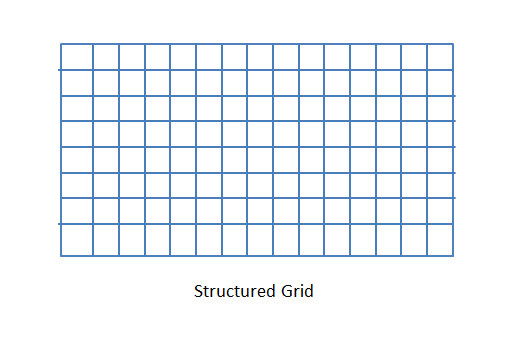
\includegraphics[width=5cm]{images/meshes/structured_grid}
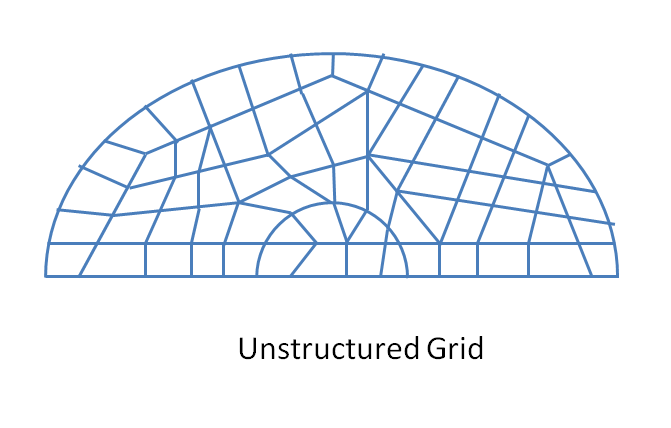
\includegraphics[width=5cm]{images/meshes/unstructured_grid}
\end{center}

On the following figure are shown various triangle- tetrahedron-based meshes. 
These are obviously better suited for simulations of complex geometries:
\begin{center}
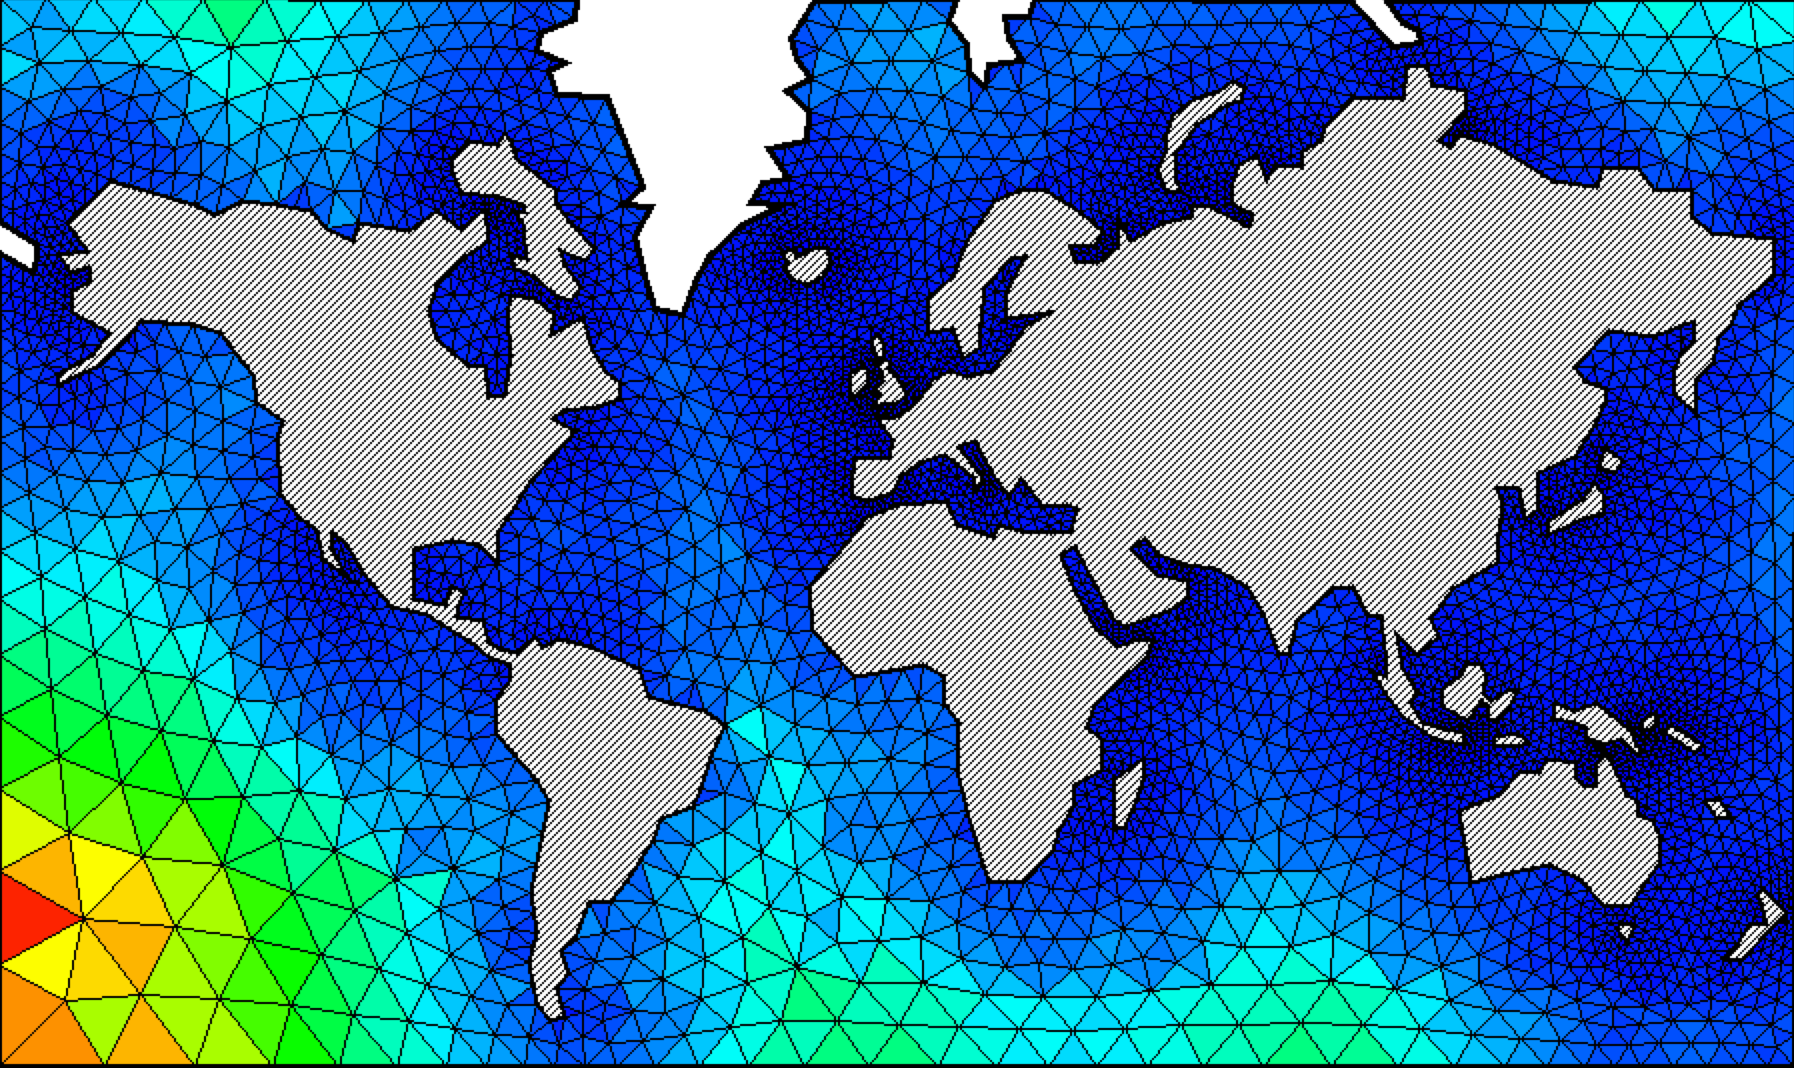
\includegraphics[height=4cm]{images/meshes/tr1.png}
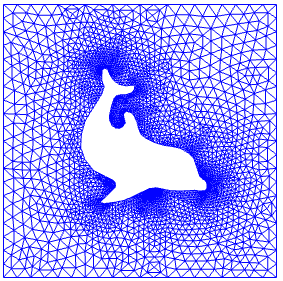
\includegraphics[height=4cm]{images/meshes/dolfin.png}
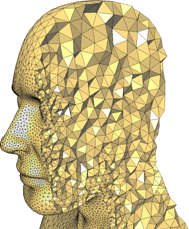
\includegraphics[height=4cm]{images/meshes/tetra.png}\\
{\color{red} add more examples}
\end{center}


Let us now focus on the case of a rectangular computational domain of size 
{\tt Lx} $\times$ {\tt Ly} with a regular mesh composed of {\tt nelx}$\times${\tt nely}={\tt nel}
   quadrilaterals.  
There are then {\tt nnx}$\times${\tt nny}={\tt nnp} grid points.
The elements are of size {\tt hx}$\times${\tt hy} with {\tt hx}={\tt Lx}/{\tt nelx}.

We have no reason to come up with an irregular/ilogical node numbering so 
we can number nodes row by row or column by column as shown on the example 
hereunder of a 3$\times$2 grid:

\begin{verbatim}
8=======9======10======11       2=======5=======8======11
|       |       |       |       |       |       |       |
|  (3)  |  (4)  |  (5)  |       |  (1)  |  (3)  |  (5)  |
|       |       |       |       |       |       |       |
4=======5=======6=======7       1=======4=======7======10
|       |       |       |       |       |       |       |
|  (0)  |  (1)  |  (2)  |       |  (0)  |  (2)  |  (4)  |
|       |       |       |       |       |       |       |
0=======1=======2=======3       0=======3=======6=======9

     "row by row"                  "column by column"
\end{verbatim}

The numbering of the elements themselves could be done in a somewhat chaotic 
way but we follow the numbering of the nodes for simplicity.
The row by row option is the adopted one in \fieldstone and the coordinates of the 
points are computed as follows:

\begin{lstlisting}
x = np.empty(nnp, dtype=np.float64)
y = np.empty(nnp, dtype=np.float64)
counter = 0
for j in range(0,nny):
    for i in range(0,nnx):
        x[counter]=i*hx
        y[counter]=j*hy
        counter += 1
\end{lstlisting}
The inner loop has {\tt i} ranging from {\tt 0} to {\tt nnx-1} first for {\tt j}=0, 1, ...
up to {\tt nny-1} which indeed corresponds to the row by row numbering.

\index{connectivity array} 
We now turn to the connectivity. As mentioned before, this is a structured mesh so that the so-called
connectivity array, named {\tt icon} in our case, can be filled easily. For each element we need
to store the node identities of its vertices. Since there are {\tt nel} elements and {\tt m=4} corners, 
this is a {\tt m}$\times${\tt nel} array. The algorithm goes as follows:

\begin{lstlisting}
icon =np.zeros((m,nel),dtype=np.int16)
counter = 0
for j in range(0,nely):
    for i in range(0,nelx):
        icon[0,counter] = i + j * nnx 
        icon[1,counter] = i + 1 + j * nnx 
        icon[2,counter] = i + 1 + (j + 1) * nnx 
        icon[3,counter] = i + (j + 1) * nnx 
        counter += 1
\end{lstlisting}

In the case of the 3$\times$2 mesh, the {\tt icon} is filled as follows:
\begin{center}
\begin{tabular}{ccccccc}
element id$\rightarrow$ &0 &1&2&3&4&5 \\
node id$\downarrow$ \\
0& 0& 1& 2& 4& 5  &6\\
1& 1& 2& 3& 5& 6  &7\\
2& 5& 6& 7& 9& 10 &11\\
3& 4& 5& 6& 8& 9  &10\\
\end{tabular}
\end{center}
It is to be understood as follows: element $\#4$ is composed of nodes 5, 6, 10 and 9.
Note that nodes are always stored in a counter clockwise manner, starting at the bottom left.
This is very important since the corresponding basis functions and their derivatives 
will be labelled accordingly.

In three dimensions things are very similar. The mesh now counts 
{\tt nelx}$\times${\tt nely}$\times${\tt nelz}={\tt nel} elements which represent 
a cuboid of size {\tt Lx}$\times${\tt Ly}$\times${\tt Lz}.
The position of the nodes is obtained as follows:
\begin{lstlisting}
x = np.empty(nnp,dtype=np.float64)
y = np.empty(nnp,dtype=np.float64)
z = np.empty(nnp,dtype=np.float64)
counter=0
for i in range(0,nnx):
    for j in range(0,nny):
        for k in range(0,nnz):
            x[counter]=i*hx
            y[counter]=j*hy
            z[counter]=k*hz
            counter += 1
\end{lstlisting}
The connectivity array is now of size {\tt m}$\times${\tt nel} with {\tt m=8}:
\begin{lstlisting}
icon =np.zeros((m,nel),dtype=np.int16)
counter = 0
for i in range(0,nelx):
    for j in range(0,nely):
        for k in range(0,nelz):
            icon[0,counter]=nny*nnz*(i  )+nnz*(j  )+k
            icon[1,counter]=nny*nnz*(i+1)+nnz*(j  )+k
            icon[2,counter]=nny*nnz*(i+1)+nnz*(j+1)+k
            icon[3,counter]=nny*nnz*(i  )+nnz*(j+1)+k
            icon[4,counter]=nny*nnz*(i  )+nnz*(j  )+k+1
            icon[5,counter]=nny*nnz*(i+1)+nnz*(j  )+k+1
            icon[6,counter]=nny*nnz*(i+1)+nnz*(j+1)+k+1
            icon[7,counter]=nny*nnz*(i  )+nnz*(j+1)+k+1
            counter += 1
\end{lstlisting}

{\color{red} produce drawing of node numbering}


\newpage
\subsection{The value of the timestep}

\subsection{Tracking materials}

\subsection{Visco-Plasticity}

\subsection{Picard and Newton}

\subsection{The choice of solvers}

\subsection{The SUPG formulation for the energy equation}

\subsection{Tracking materials and/or interfaces}

\subsection{Dealing with a free surface}



\newpage
\subsection{Pressure smoothing}

It has been widely documented that the use of the $Q_1 \times P_0$ element is not without problems. Aside from the 
consequences it has on the FE matrix properties, we will here focus on another unavoidable side effect: the spurious pressure 
checkerboard modes. \index{pressure smoothing} \index{checkerboard}

These modes have been thoroughly analysed \cite{grsi94,chpc95,sagl81a,sagl81b}.
They can be filtered out \cite{chpc95} or simply smoothed \cite{legs79}.

On the following figure (a,b), pressure fields for the lid driven cavity experiment 
are presented for both an even and un-even number of elements. We see that 
the amplitude of the modes can sometimes be so large that the 'real' pressure is 
not visible and that something as simple as the number of elements in the 
domain can trigger those or not at all.

\begin{center}
a)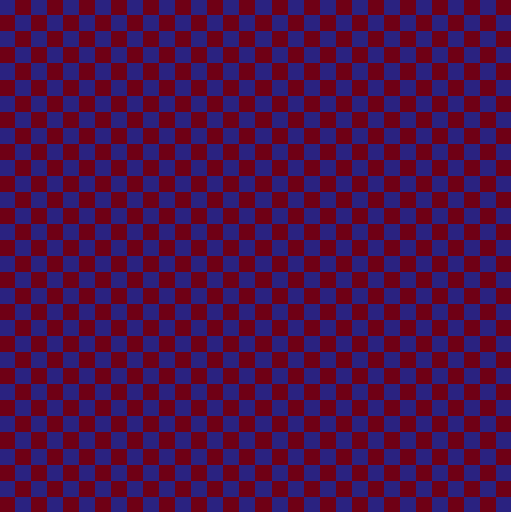
\includegraphics[width=3cm]{images/checkerboard/p_el}
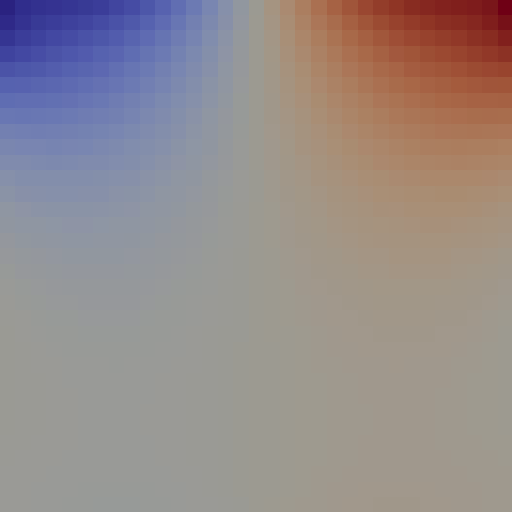
\includegraphics[width=3cm]{images/checkerboard/p_el_33x33}
b)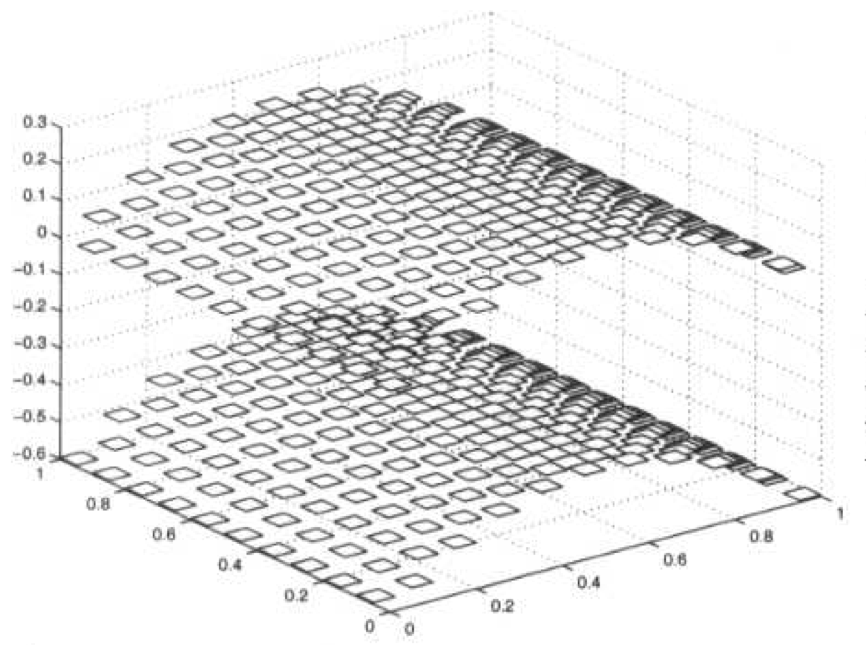
\includegraphics[width=5cm]{images/checkerboard/press_doneahuerta}
c)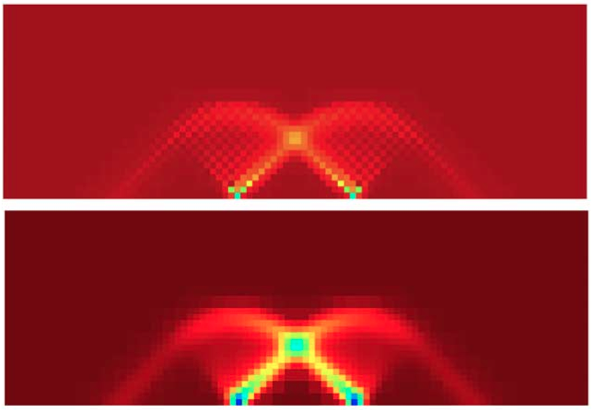
\includegraphics[width=5cm]{images/checkerboard/douarpunch}\\
{\small a) element pressure for a 32x32 grid and for a 33x33 grid;\\ 
b) image from \cite[p307]{dohu} for a manufactured solution;\\ 
c) elemental pressure and smoothed pressure for the punch experiment \cite{thfb08}}
\end{center}

The easiest post-processing step that can be used (especially when a regular grid is used) 
is explained in \cite{thfb08}: "The element-to-node interpolation is performed by
averaging the elemental values from elements common to each node; 
the node-to-element interpolation is performed
by averaging the nodal values element-by-element. This
method is not only very efficient but produces a smoothing
of the pressure that is adapted to the local density of the
octree. Note that these two steps can be repeated until a
satisfying level of smoothness (and diffusion) of the pres-
sure field is attained."

In the codes which rely on the $Q_1 \times P_0$ element, the (elemental) pressure
is simply defined as 
\begin{lstlisting}
p=np.zeros(nel,dtype=np.float64)  
\end{lstlisting}
while the nodal pressure is then defined as 
\begin{lstlisting}
q=np.zeros(nnp,dtype=np.float64)  
\end{lstlisting}
The element-to-node algorithm is then simply (in 2D):

\begin{lstlisting}
count=np.zeros(nnp,dtype=np.int16)  
for iel in range(0,nel):
    q[icon[0,iel]]+=p[iel]
    q[icon[1,iel]]+=p[iel]
    q[icon[2,iel]]+=p[iel]
    q[icon[3,iel]]+=p[iel]
    count[icon[0,iel]]+=1
    count[icon[1,iel]]+=1
    count[icon[2,iel]]+=1
    count[icon[3,iel]]+=1
q=q/count
\end{lstlisting}

{\color{red} produce figure to explain this}

{\color{red} link to proto paper }

{\color{red} link to least square and nodal derivatives}




\newpage
\subsection{Pressure normalisation}




\newpage
\subsection{Static condensation} \index{static condensation}





\newpage
{\bf To Do}:

write about impose bc on el matrix

full compressible 

total energy calculations

constraints

compositions, marker chain

van keken initial value with deformed mesh

free-slip bc on annulus and sphere . See for example p540 Gresho and Sani book.

non-linear rheologies (two layer brick spmw16, tosn15) 

Picard vs Newton

markers

Schur complement approach

periodic boundary conditions

open boundary conditions

consistent boundary flux (CBF)

free surface 

SUPG

zaleski disk advection

Busse convection pb, compare with aspect 

cvi !!!

pure elastic 

including phase changes (w. R. Myhill)

discontinuous galerkin

formatting of code style

navier-stokes ? (LUKAS)


compute strainrate in middle of element or at quad point for punch?

GEO1442 code 

GEO1442 indenter setup in plane ?

in/out flow on sides for lith modelling

\noindent Problems to solve:

colorscale 

better yet simple matrix storage ?


\newpage
%%%%%%%%%%%%%%%%%%%%%%%%%%%%%%%%%%%%%%%%%%%%%%%%%%%%%%%%%%%%%%%%%%%%%%%%%%%%%%%
\section{{\tt fieldstone}: simple analytical solution \label{f1}}

From \cite{dohu}. In order to illustrate the behavior of selected mixed finite elements in the solution 
of stationary Stokes flow,  we consider a two-dimensional problem 
in the square domain $\Omega=[0,1]\times[0,1]$, which possesses a closed-form analytical 
solution. The problem consists of determining the velocity field ${\bm v} = (u,v)$ and the 
pressure $p$ such that 
\[
-\nu \Delta {\bm v} + {\bm \nabla} p = {\bm b}  \quad\quad {\rm in} \; \Omega
\]
\[
{\bm \nabla} \cdot {\bm v} = 0 \quad\quad {\rm in} \; \Omega
\]
\[
{\bm v}={\bm 0} \quad\quad {\rm on} \; \Gamma
\]
where the fluid viscosity is taken as $\nu=1$. The components of the body force ${\bm b}$ are prescribed as 
\begin{eqnarray}
b_x &=& (12 - 24y) x^4 + (-24 + 48y) x^3 + (-48y + 72y^2 - 48 y^3 + 12) x^2 \nonumber\\
    && + (-2 + 24y -72y^2+48y^3)x + 1-4y + 12y^2-8y^3 \nonumber\\ 
b_y &=& (8 - 48y + 48 y^2) x^3 + (-12 + 72y - 72y^2) x^2  \nonumber\\
    && + (4 - 24y + 48y^2 - 48y^3 + 24y^4) x - 12y^2 + 24y^3 - 12y^4  \nonumber
\end{eqnarray}
With this prescribed body force, the exact solution is 
\begin{eqnarray}
u(x,y) &=& x^2(1- x)^2 (2y - 6y^2 + 4y^3)  \nonumber\\
v(x,y) &=& -y^2 (1 - y)^2 (2x - 6x^2 + 4x^3) \nonumber\\
p(x,y) &=& x(1 -x)- 1/6 \nonumber 
\end{eqnarray}
Note that the pressure obeys $\int_{\Omega} p \; d\Omega = 0$

\fbox{
\parbox{10cm}{{\bf features}
\begin{itemize}
\item $Q_1\times P_0$ element
\item incompressible flow
\item penalty formulation
\item Dirichlet boundary conditions (no-slip)
\item direct solver
\item isothermal
\item isoviscous
\item analytical solution
\end{itemize}
}}

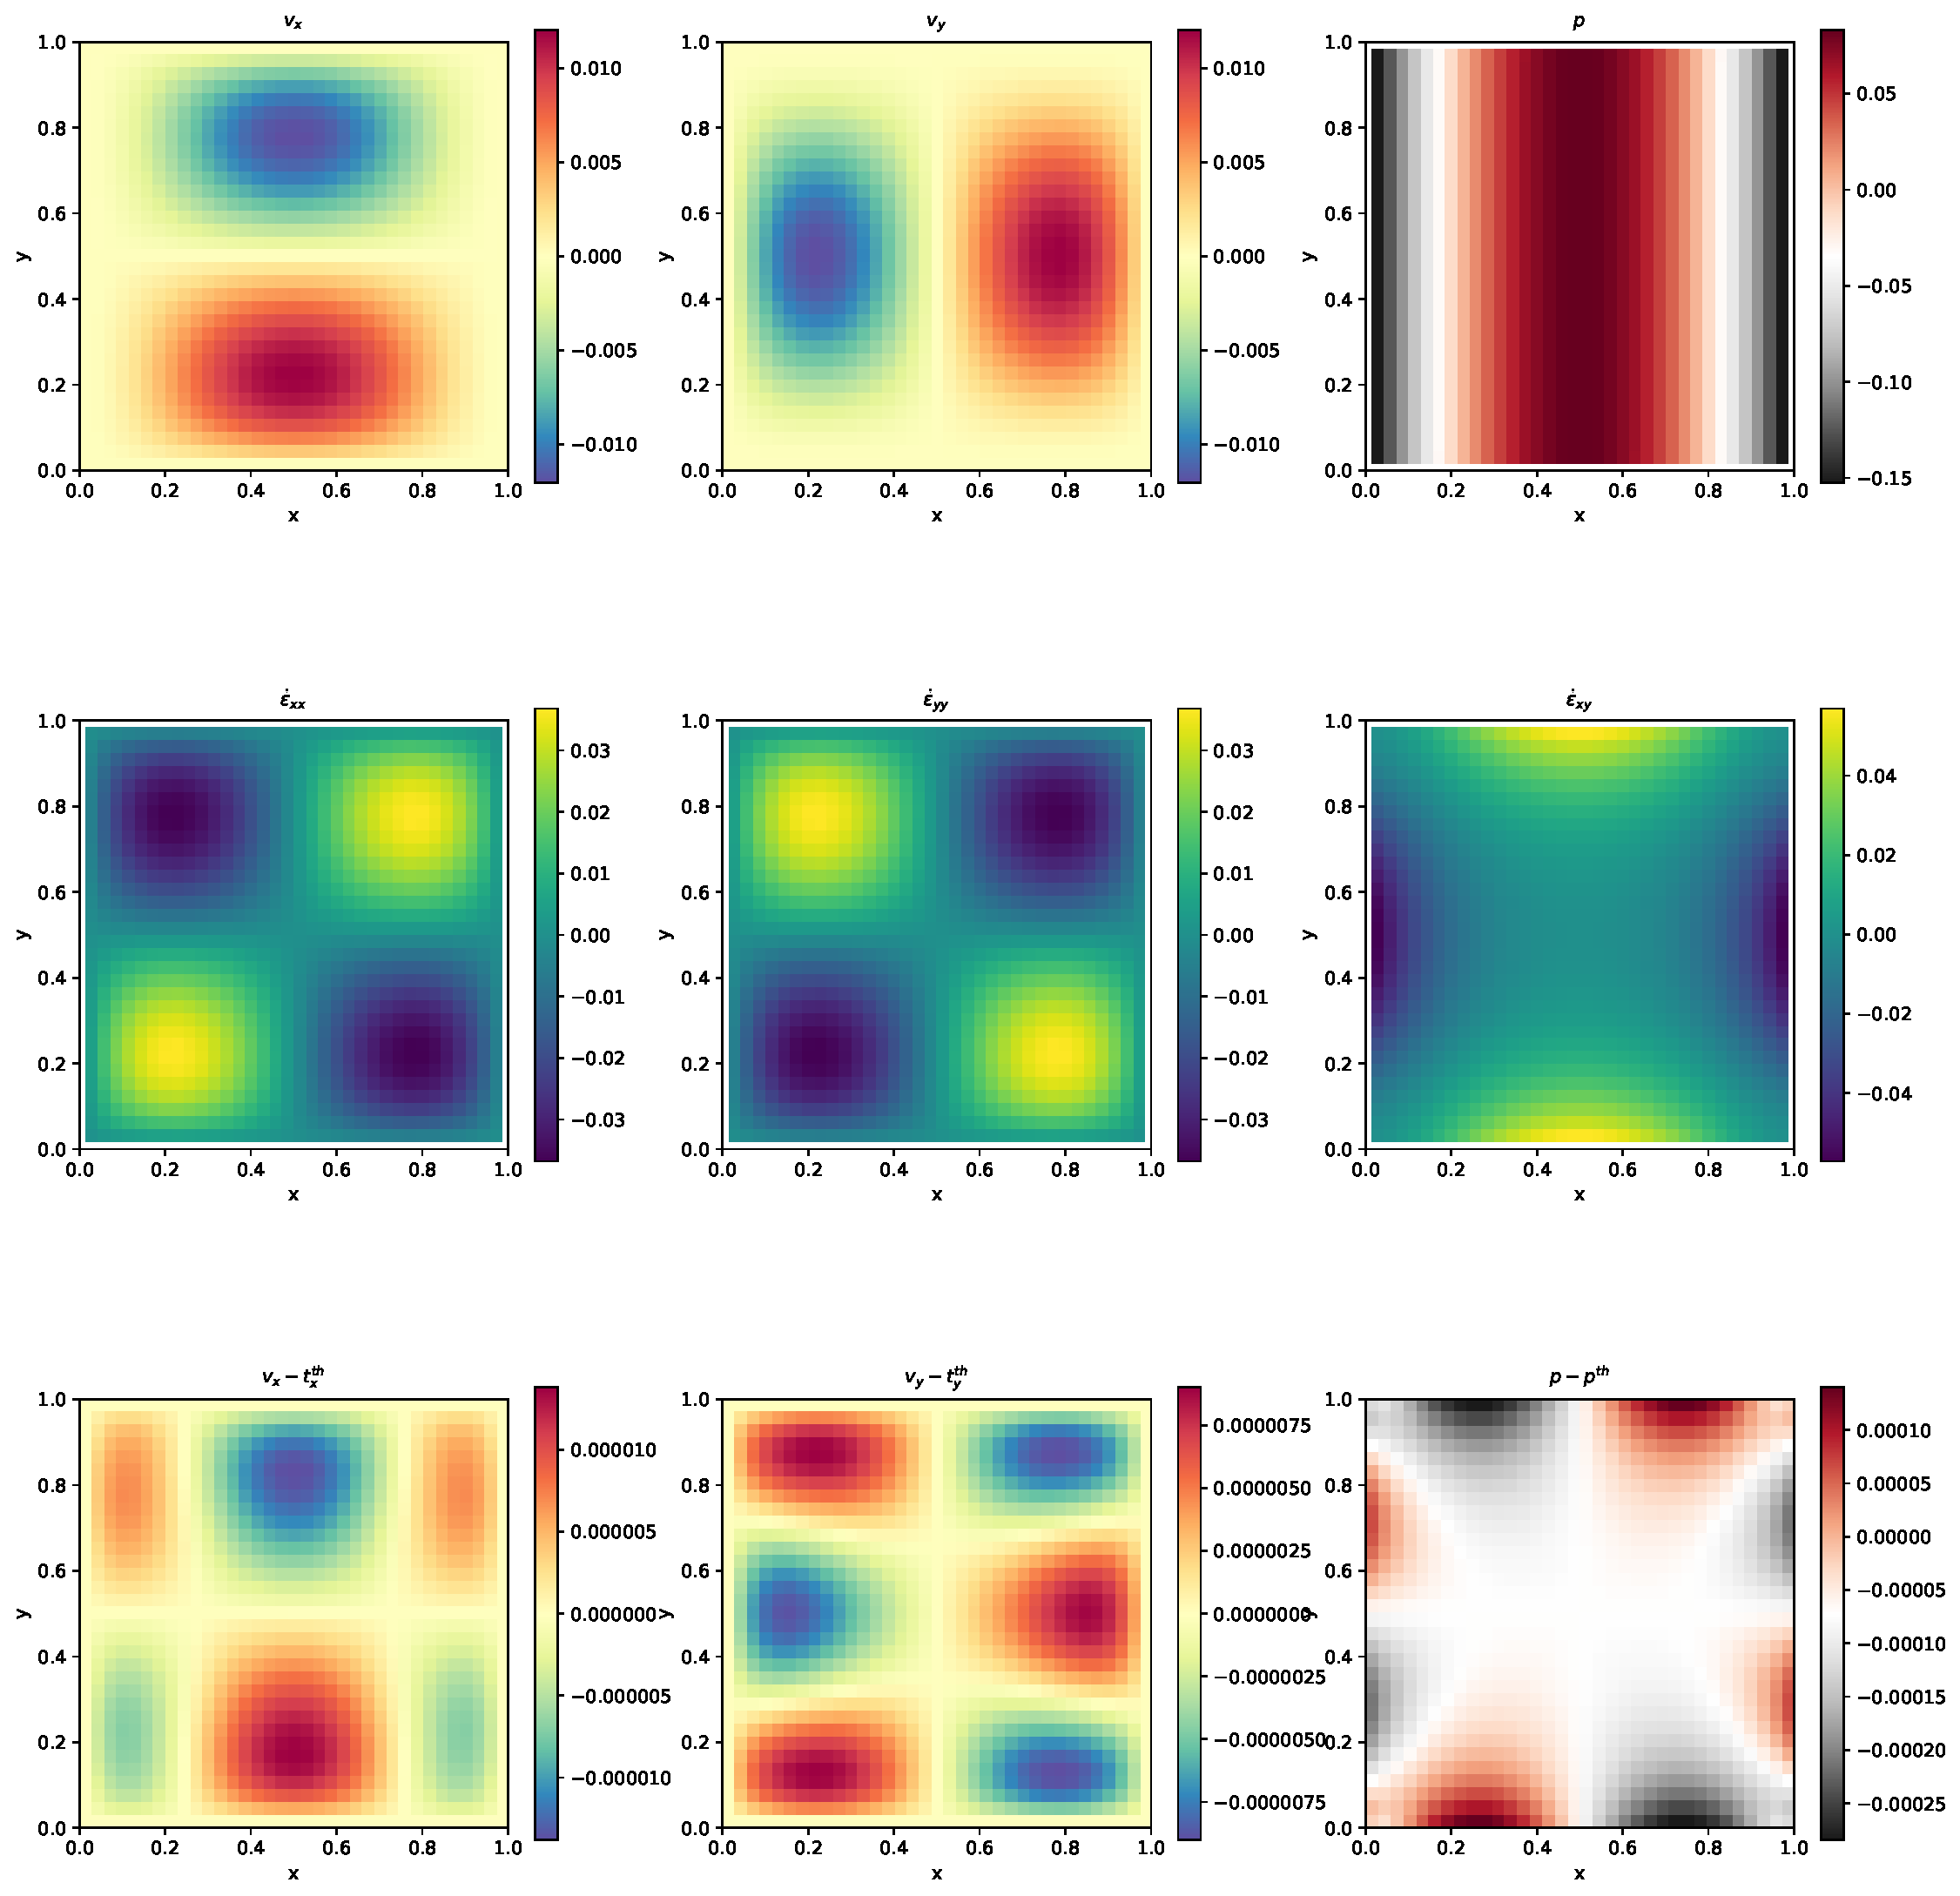
\includegraphics[width=16cm]{python_codes/fieldstone/solution.pdf}

\begin{center}
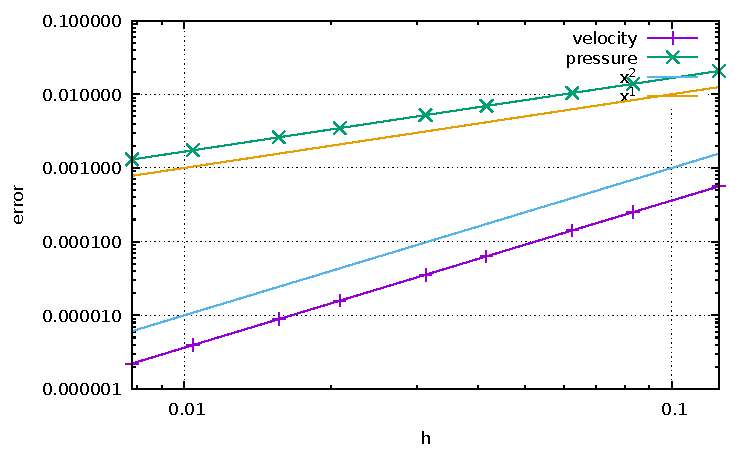
\includegraphics[width=12cm]{python_codes/fieldstone/errors.pdf}\\
Quadratic convergence for velocity error, 
linear convergence for pressure error, as expected.
\end{center}

ToDo:

pressure normalisation?

different cmat, a la schmalholz

To go further:
\begin{enumerate}
\item make your own analytical solution
\end{enumerate}


\newpage
%%%%%%%%%%%%%%%%%%%%%%%%%%%%%%%%%%%%%%%%%%%%%%%%%%%%%%%%%%%%%%%%%%%%%%%%%%%%%%%
\section{{\tt fieldstone}: Stokes sphere }

Viscosity and density directly computed at the quadrature points.

\fbox{
\parbox{10cm}{{\bf features}
\begin{itemize}
\item $Q_1\times P_0$ element
\item incompressible flow
\item penalty formulation \index{penalty formulation}
\item Dirichlet boundary conditions (free-slip)
\item isothermal
\item non-isoviscous
\item buoyancy-driven flow \index{buoyancy-driven flow}
\item Stokes sphere \index{Stokes sphere}
\end{itemize}
}}

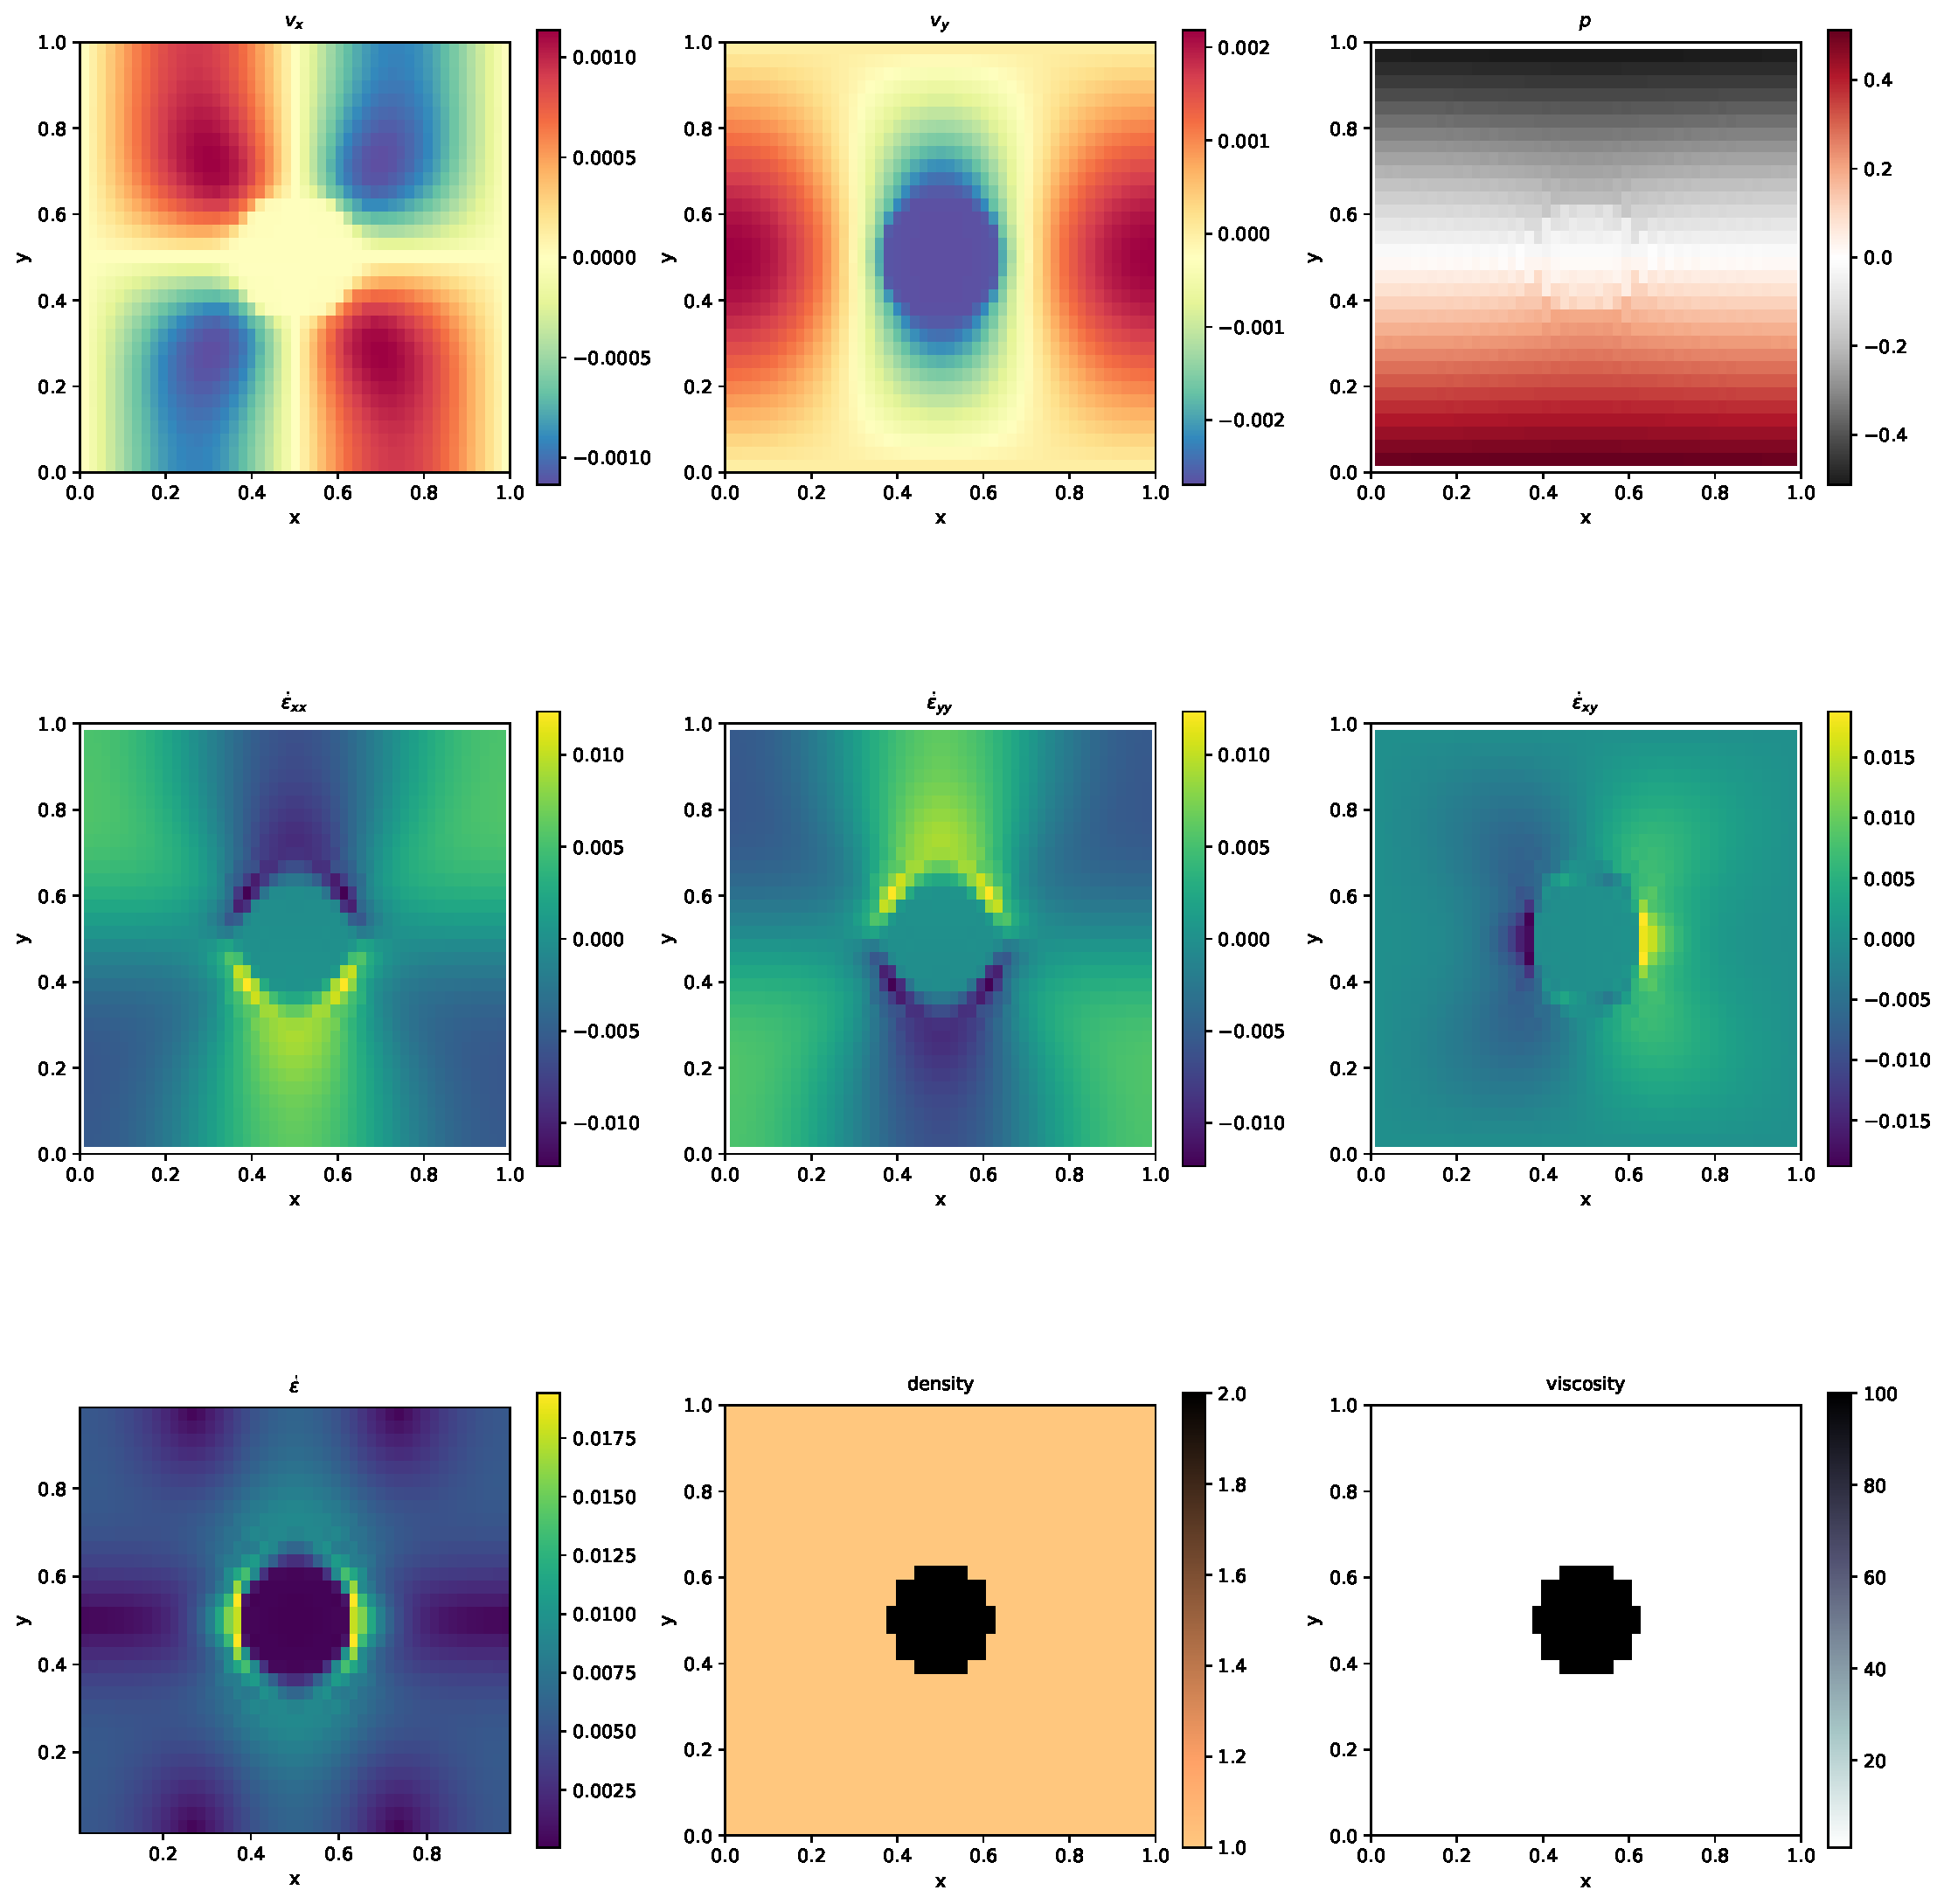
\includegraphics[width=16cm]{python_codes/fieldstone_stokes_sphere/solution.pdf}



\newpage
%%%%%%%%%%%%%%%%%%%%%%%%%%%%%%%%%%%%%%%%%%%%%%%%%%%%%%%%%%%%%%%%%%%%%%%%%%%%%%%
\section{{\tt fieldstone}: Convection in a 2D box}

This benchmark deals with the 2-D thermal convection of a fluid 
of infinite Prandtl number in a rectangular closed cell.
In what follows, I carry out the case 1a, 1b, and 1c experiments as shown in \cite{blbc89}:
steady convection with constant viscosity in a square box.

The temperature is fixed to zero on top and to $\Delta T$ at the bottom, 
with reflecting symmetry at the sidewalls (i.e. $\partial_x T=0$) 
and there are no internal heat sources. 
Free-slip conditions are implemented on all boundaries. 

The Rayleigh number is given by
\begin{equation}
Ra = \frac{\alpha g_y \Delta T h^3 }{\kappa \nu}
=\frac{\alpha g_y \Delta T h^3 \rho^2 c_p}{k \mu}
\end{equation}

In what follows, I use the following parameter values:  %, as given in \cite{krhb12}:
$L_x=L_y=1$,$\rho_0=c_P=k=\mu=1$, $T_0=0$, $\alpha=10^{-2}$, $g=10^{2}Ra$
and I run the model with $Ra=10^4,10^{5}$ and $10^6$.

The initial temperature field is given by 
\begin{equation}
T(x,y)=(1-y) - 0.01\cos(\pi x) \sin(\pi z)
\end{equation}
The perturbation in the initial temperature fields leads to 
a perturbation of the density field and sets the fluid in motion. 

Depending on the initial Rayleigh number, the system ultimately reaches a 
steady state after some time. 

The Nusselt number (i.e. the mean surface temperature gradient over mean bottom temperature)
is computed as follows \cite{blbc89}:
\begin{equation}
Nu = L_y \frac{\int \frac{\partial T}{\partial y}(y=L_y) dx  }{\int T(y=0) dx}
\label{eqNu}
\end{equation}
Note that in our case the denominator is equal to 1 since $L_x=1$ and the temperature at the 
bottom is prescribed to be 1.

Finally, the steady state root mean square velocity and Nusselt number measurements
are indicated in Table \ref{tab_bl} alongside those of \cite{blbc89} and \cite{tack94}.
(Note that this benchmark was also carried out and published in  
other publications \cite{trha98,albe00,gery10,dawk11,lezh11} but since they did not provide  a complete set
of measurement values, they are not included in the table.)

\begin{center}
\begin{tabular}{llcc}
\hline
          &           & Blankenbach et al & Tackley \cite{tack94}    \\
\hline
\hline
$Ra=10^4$ & $V_{rms}$ &  $42.864947  \pm 0.000020$ & 42.775 \\
          & $Nu$      &  $4.884409   \pm 0.000010$ & 4.878  \\
$Ra=10^5$ & $V_{rms}$ &  $193.21454  \pm 0.00010 $ & 193.11 \\
          & $Nu$      &  $10.534095  \pm 0.000010$ & 10.531 \\
$Ra=10^6$ & $V_{rms}$ &  $833.98977  \pm 0.00020 $ & 833.55 \\
          & $Nu$      &  $21.972465  \pm 0.000020$ & 21.998 \\
\hline
\end{tabular}\\
{\small Steady state Nusselt number $Nu$ and $V_{rms}$ measurements as reported in the literature. }
\end{center}






\fbox{
\parbox{10cm}{{\bf features}
\begin{itemize}
\item $Q_1\times P_0$ element
\item incompressible flow
\item penalty formulation
\item Dirichlet boundary conditions (free-slip)
\item Boussinesq approximation
\item direct solver
\item non-isothermal
\item buoyancy-driven flow
\item isoviscous
\item CFL-condition
\end{itemize}
}}

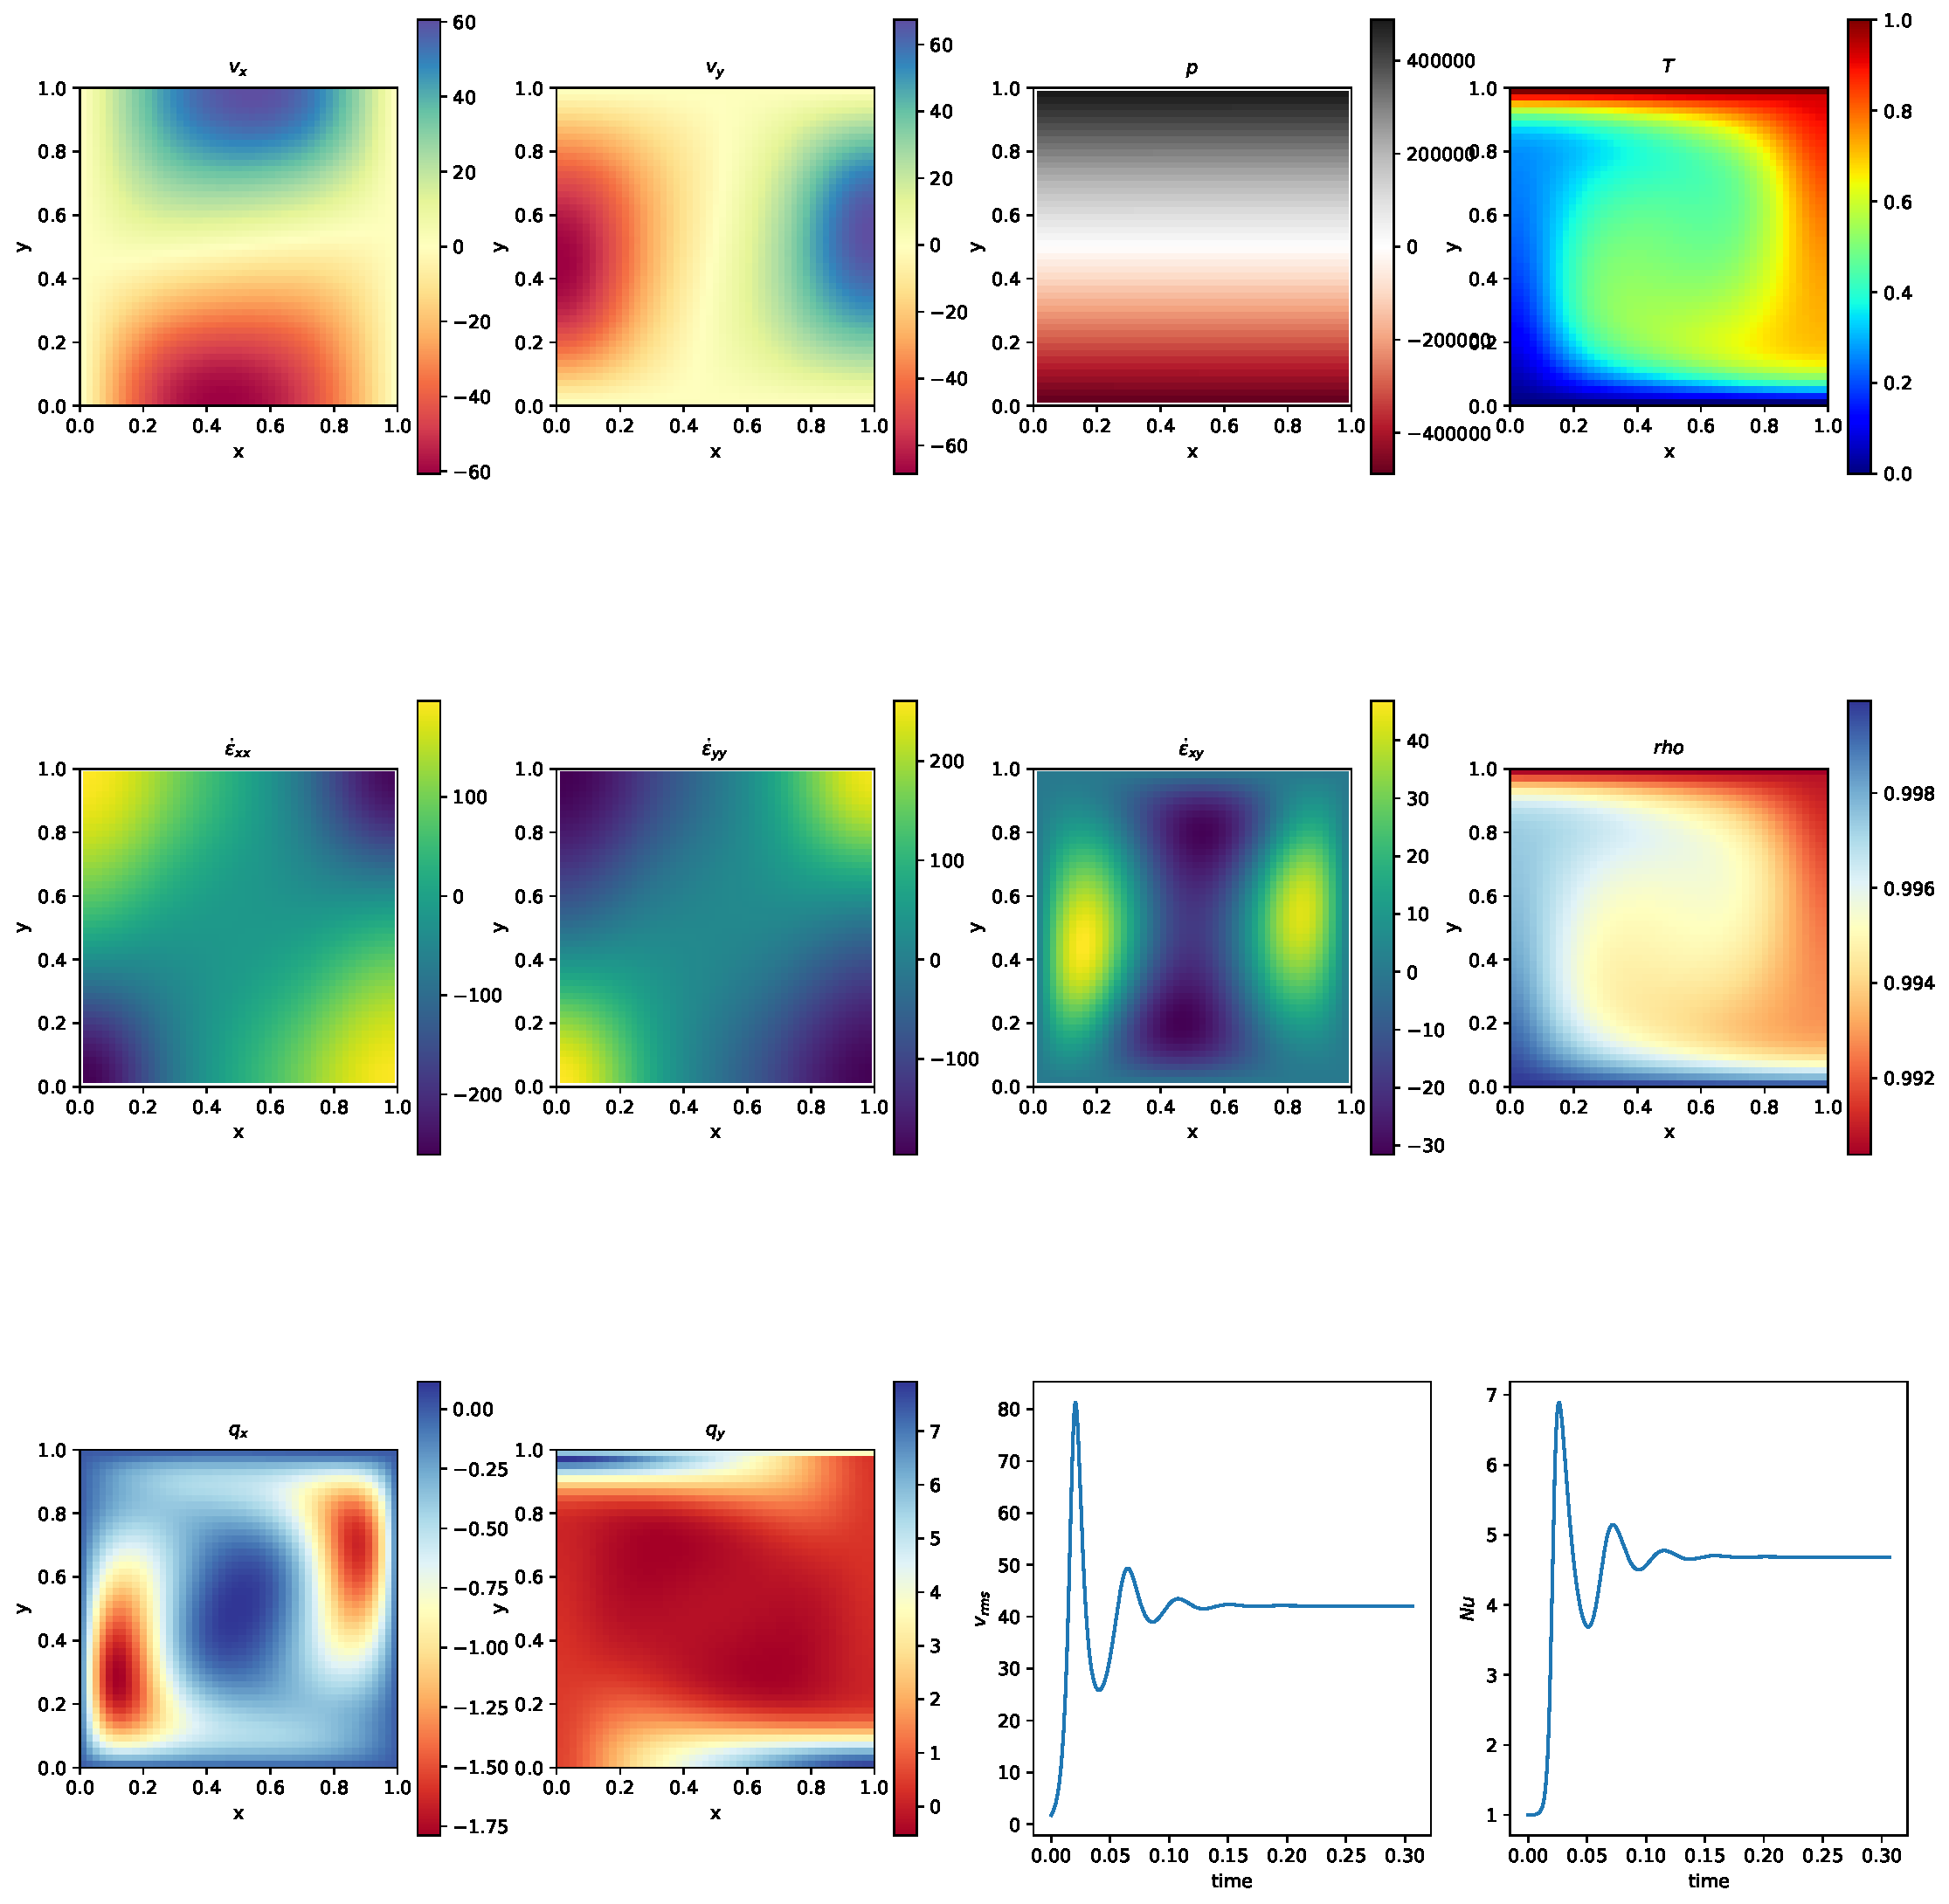
\includegraphics[width=16cm]{python_codes/fieldstone_convection_box/solution_convection_box.pdf}

ToDo:

implement steady state criterion

reach steady state

do Ra=1e4, 1e5, 1e6

plot against blankenbach paper and aspect

look at critical Ra number


\newpage
%%%%%%%%%%%%%%%%%%%%%%%%%%%%%%%%%%%%%%%%%%%%%%%%%%%%%%%%%%%%%%%%%%%%%%%%%%%%%%%
\section{{\tt fieldstone}: The lid driven cavity}


The lid driven cavity is a famous Computational Fluid Dynamics test case and 
has been studied in countless publications with a wealth of numerical techniques
(see \cite{ertu09} for a succinct review) and also in the laboratory \cite{kost84}.

It models a plane flow of an isothermal isoviscous fluid in a rectangular (usually square) lid-driven cavity. 
The boundary conditions are indicated in the Fig. \ref{fig_ldc}a. The gravity is set to zero.

%---------------------------------------------------------
\subsection{the lid driven cavity problem ({\tt ldc=0})}
In the standard case, the upper side of the cavity moves in its own plane at unit speed, while the other sides are fixed.
This thereby introduces a discontinuity in the boundary conditions at the two upper corners of the cavity and yields
an uncertainty as to which boundary (side or top) the corner points belong to. 
In this version of the code the top corner nodes are considered to be part of the lid. If these are excluded 
the recovered pressure showcases and extremely large checkboard pattern.

This benchmark is usually dicussed in the context of low to very high Reynolds number with the full 
Navier-Stokes equations being solved (with the noticeable exception of \cite{sagl81a,sagl81b,chpc95,eid2005}
which focus on the Stokes equation). 
In the case of the incompressible Stokes flow, 
the absence of inertia renders this problem instantaneous so that only one time step is needed.

%---------------------------------------------------------
\subsection{the lid driven cavity problem - regularisation I ({\tt ldc=1})}

We avoid the top corner nodes issue altogether by  
prescribing the horizontal velocity of the lid as follows: 
\begin{equation}
u(x)=x^2(1-x)^2.
\end{equation}
In this case the velocity and its first derivative is continuous at the corners. This is the so-called regularised lid-driven cavity problem \cite{piva94}.

%---------------------------------------------------------
\subsection{the lid driven cavity problem - regularisation II ({\tt ldc=2})}

Another regularisation was presented in \cite{dejn16}. 
Here, a regularized lid driven cavity is studied which is consistent in the sense that 
${\bm \nabla}\cdot{\bm v}=0$ 
holds also at the corners of the domain.
There are no-slip conditions at the boundaries $x=0$, $x=1$, and $y=0$. 

The velocity at $y=1$ is given by

\begin{eqnarray}
u(x) &=& 1-\frac{1}{4}\left( 1-\cos (\frac{x_1-x}{x_1}\pi)  \right)^2   \quad\quad x\in[0,x_1] \nonumber\\
u(x) &=& 1 \quad\quad x\in[x_1,1-x_1] \nonumber\\
u(x) &=& 1-\frac{1}{4}\left( 1-\cos (\frac{x-(1-x_1)}{x_1}\pi)  \right)^2   \quad\quad x\in[1-x_1,1]
\end{eqnarray}
Results are obtained with $x_1=0.1$.

\begin{center}
\fbox{
\parbox{10cm}{{\bf features}
\begin{itemize}
\item $Q_1\times P_0$ element \index{$Q_1 \times P_0$}
\item incompressible flow
\item penalty formulation \index{penalty formulation}
\item isothermal \index{isothermal}
\item isoviscous \index{isoviscous}
\end{itemize}
}}
\end{center}



\newpage
A 100x100 element grid is used. No-slip boundary conditions are prescribed on sides and
bottom. A zero vertical velocity is prescribed at the top and the exact form of the 
prescribed horizontal velocity is controlled by the {\tt ldc} parameter.

\begin{center}
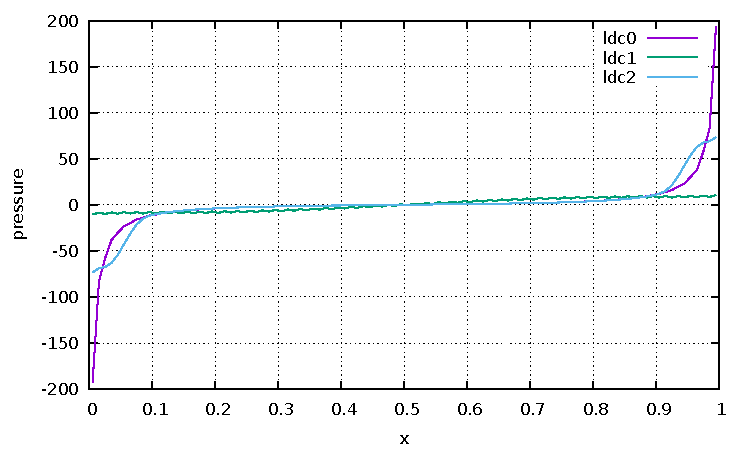
\includegraphics[width=8cm]{python_codes/fieldstone_lid_driven_cavity/results/p.pdf}\\
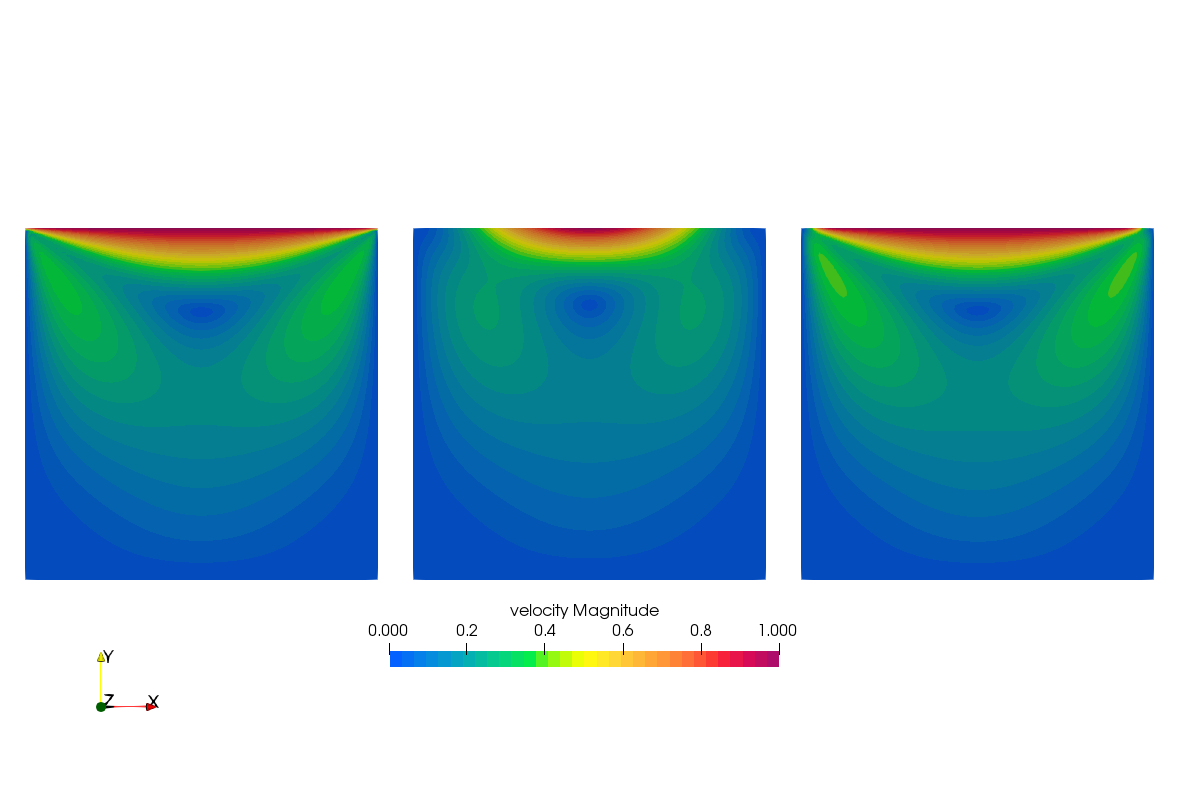
\includegraphics[width=12cm]{python_codes/fieldstone_lid_driven_cavity/results/velocities}\\
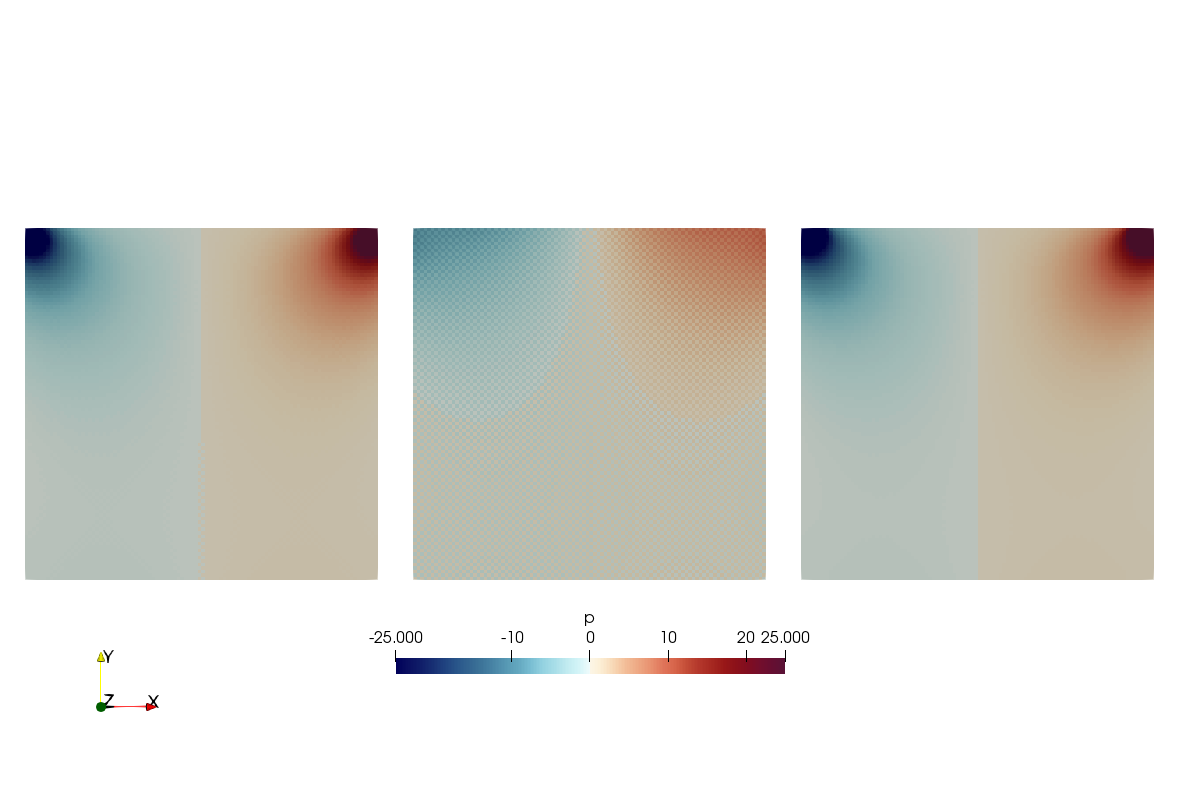
\includegraphics[width=12cm]{python_codes/fieldstone_lid_driven_cavity/results/pressures}
\end{center}




\newpage
%%%%%%%%%%%%%%%%%%%%%%%%%%%%%%%%%%%%%%%%%%%%%%%%%%%%%%%%%%%%%%%%%%%%%%%%%%%%%%%
\section{{\tt fieldstone}: solcx benchmark}

%Taken from aspect manual. 
The SolCx benchmark is intended to test the accuracy of the solution to a problem that has a large jump in the viscosity along a line through the domain. Such situations are common in geophysics: for example, the viscosity in a cold, subducting slab is much larger than in the surrounding, relatively hot mantle material.

The SolCx benchmark computes the Stokes flow field of a fluid driven by spatial density variations, subject to a spatially variable viscosity. Specifically, the domain is $\Omega = [0,1]^2$, gravity is ${\bm g} = (0,-1)^T$ and the density is given by 
\begin{equation}
\rho(x,y) = \sin(\pi y) \cos(\pi x)
\end{equation}
Boundary conditions are free slip on all of the sides of the domain and the temperature plays no role in this benchmark. 
The viscosity is prescribed as follows:
\begin{equation}
\mu(x,y) = 
\left\{
\begin{array}{lll}
1 & for & x<0.5 \\
10^6 & for & x>0.5 \\
\end{array}
\right.
\end{equation}
Note the strongly discontinuous viscosity field yields a stagnant flow 
in the right half of the domain and thereby yields a pressure discontinuity along the interface. 

The SolCx benchmark was previously used in \cite{dumg11} (references to earlier uses of the benchmark are available there) and its analytic solution is given in \cite{zhon96}. It has been carried out in \cite{krhb12} and \cite{gemd13}. 
Note that the source code which evaluates the velocity and pressure fields for both SolCx and SolKz is 
distributed as part of the open source package Underworld (\cite{moql07}, http://underworldproject.org).

In this particular example, the viscosity is computed analytically at the quadrature points (i.e. tracers are 
not used to attribute a viscosity to the element). 
If the number of elements is even in any direction, all elements (and their associated quadrature points)
have a constant viscosity($1$ or  $10^6$). If it is odd, then the elements situated 
at the viscosity jump have half their integration points with $\mu=1$ and half with $\mu=10^6$ 
(which is a pathological case since the used quadrature rule inside elements cannot represent 
accurately such a jump).  

\fbox{
\parbox{10cm}{{\bf features}
\begin{itemize}
\item $Q_1\times P_0$ element
\item incompressible flow
\item penalty formulation
\item Dirichlet boundary conditions (free-slip)
\item direct solver
\item isothermal
\item non-isoviscous
\item analytical solution
\end{itemize}
}}

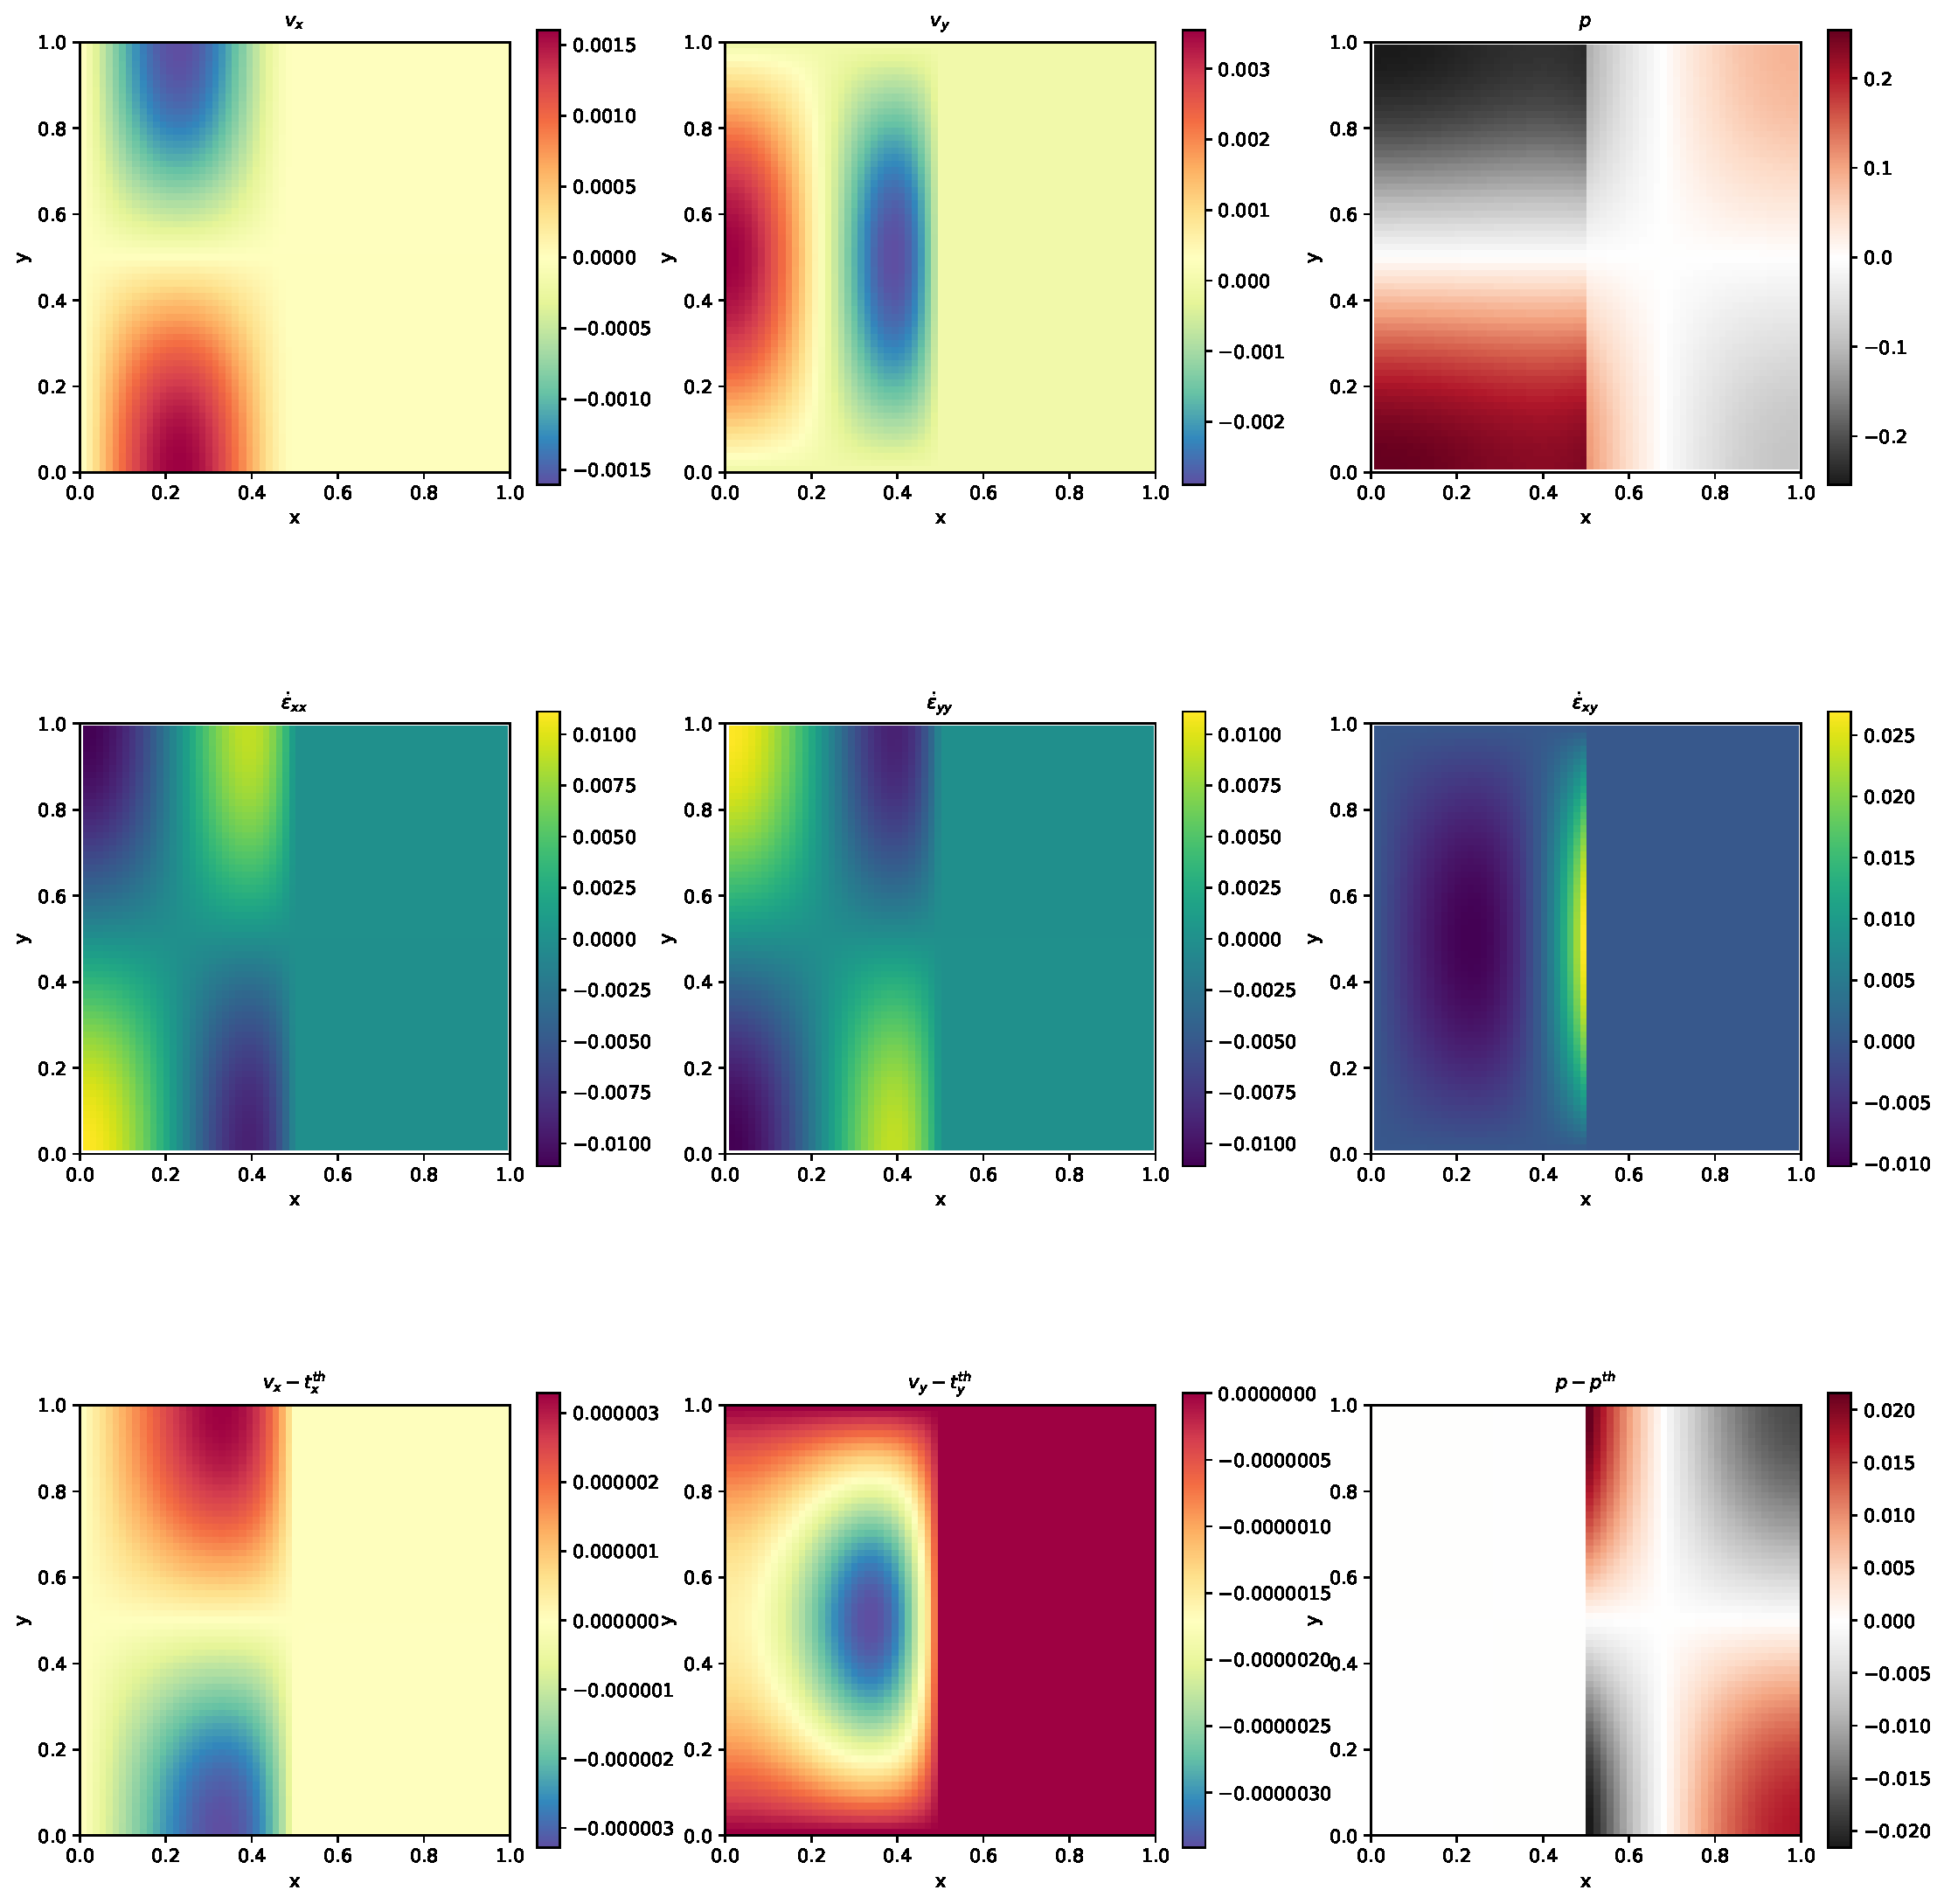
\includegraphics[width=16cm]{python_codes/fieldstone_solcx/solution.pdf}

\fbox{
\parbox{10cm}{{\bf What we learn from this}
}}





\newpage
%%%%%%%%%%%%%%%%%%%%%%%%%%%%%%%%%%%%%%%%%%%%%%%%%%%%%%%%%%%%%%%%%%%%%%%%%%%%%%%
\section{{\tt fieldstone}: solkz benchmark}

The SolKz benchmark \cite{repa87} is similar to the SolCx benchmark.
but the viscosity is now a function of the space coordinates: 
\begin{equation}
\mu(y)=\exp(By) \quad {\rm with} \quad B=13.8155
\end{equation}
It is however not a discontinuous function but grows exponentially with the vertical coordinate so that its overall variation is again $10^6$. 
The forcing is again chosen by imposing a spatially variable density variation as follows:
\begin{equation}
\rho(x,y)=\sin(2y) \cos(3\pi x)
\end{equation}
Free slip boundary conditions are imposed on all sides of the domain.
This benchmark is presented in \cite{zhon96} as well and is studied in \cite{dumg11} and \cite{gemd13}.

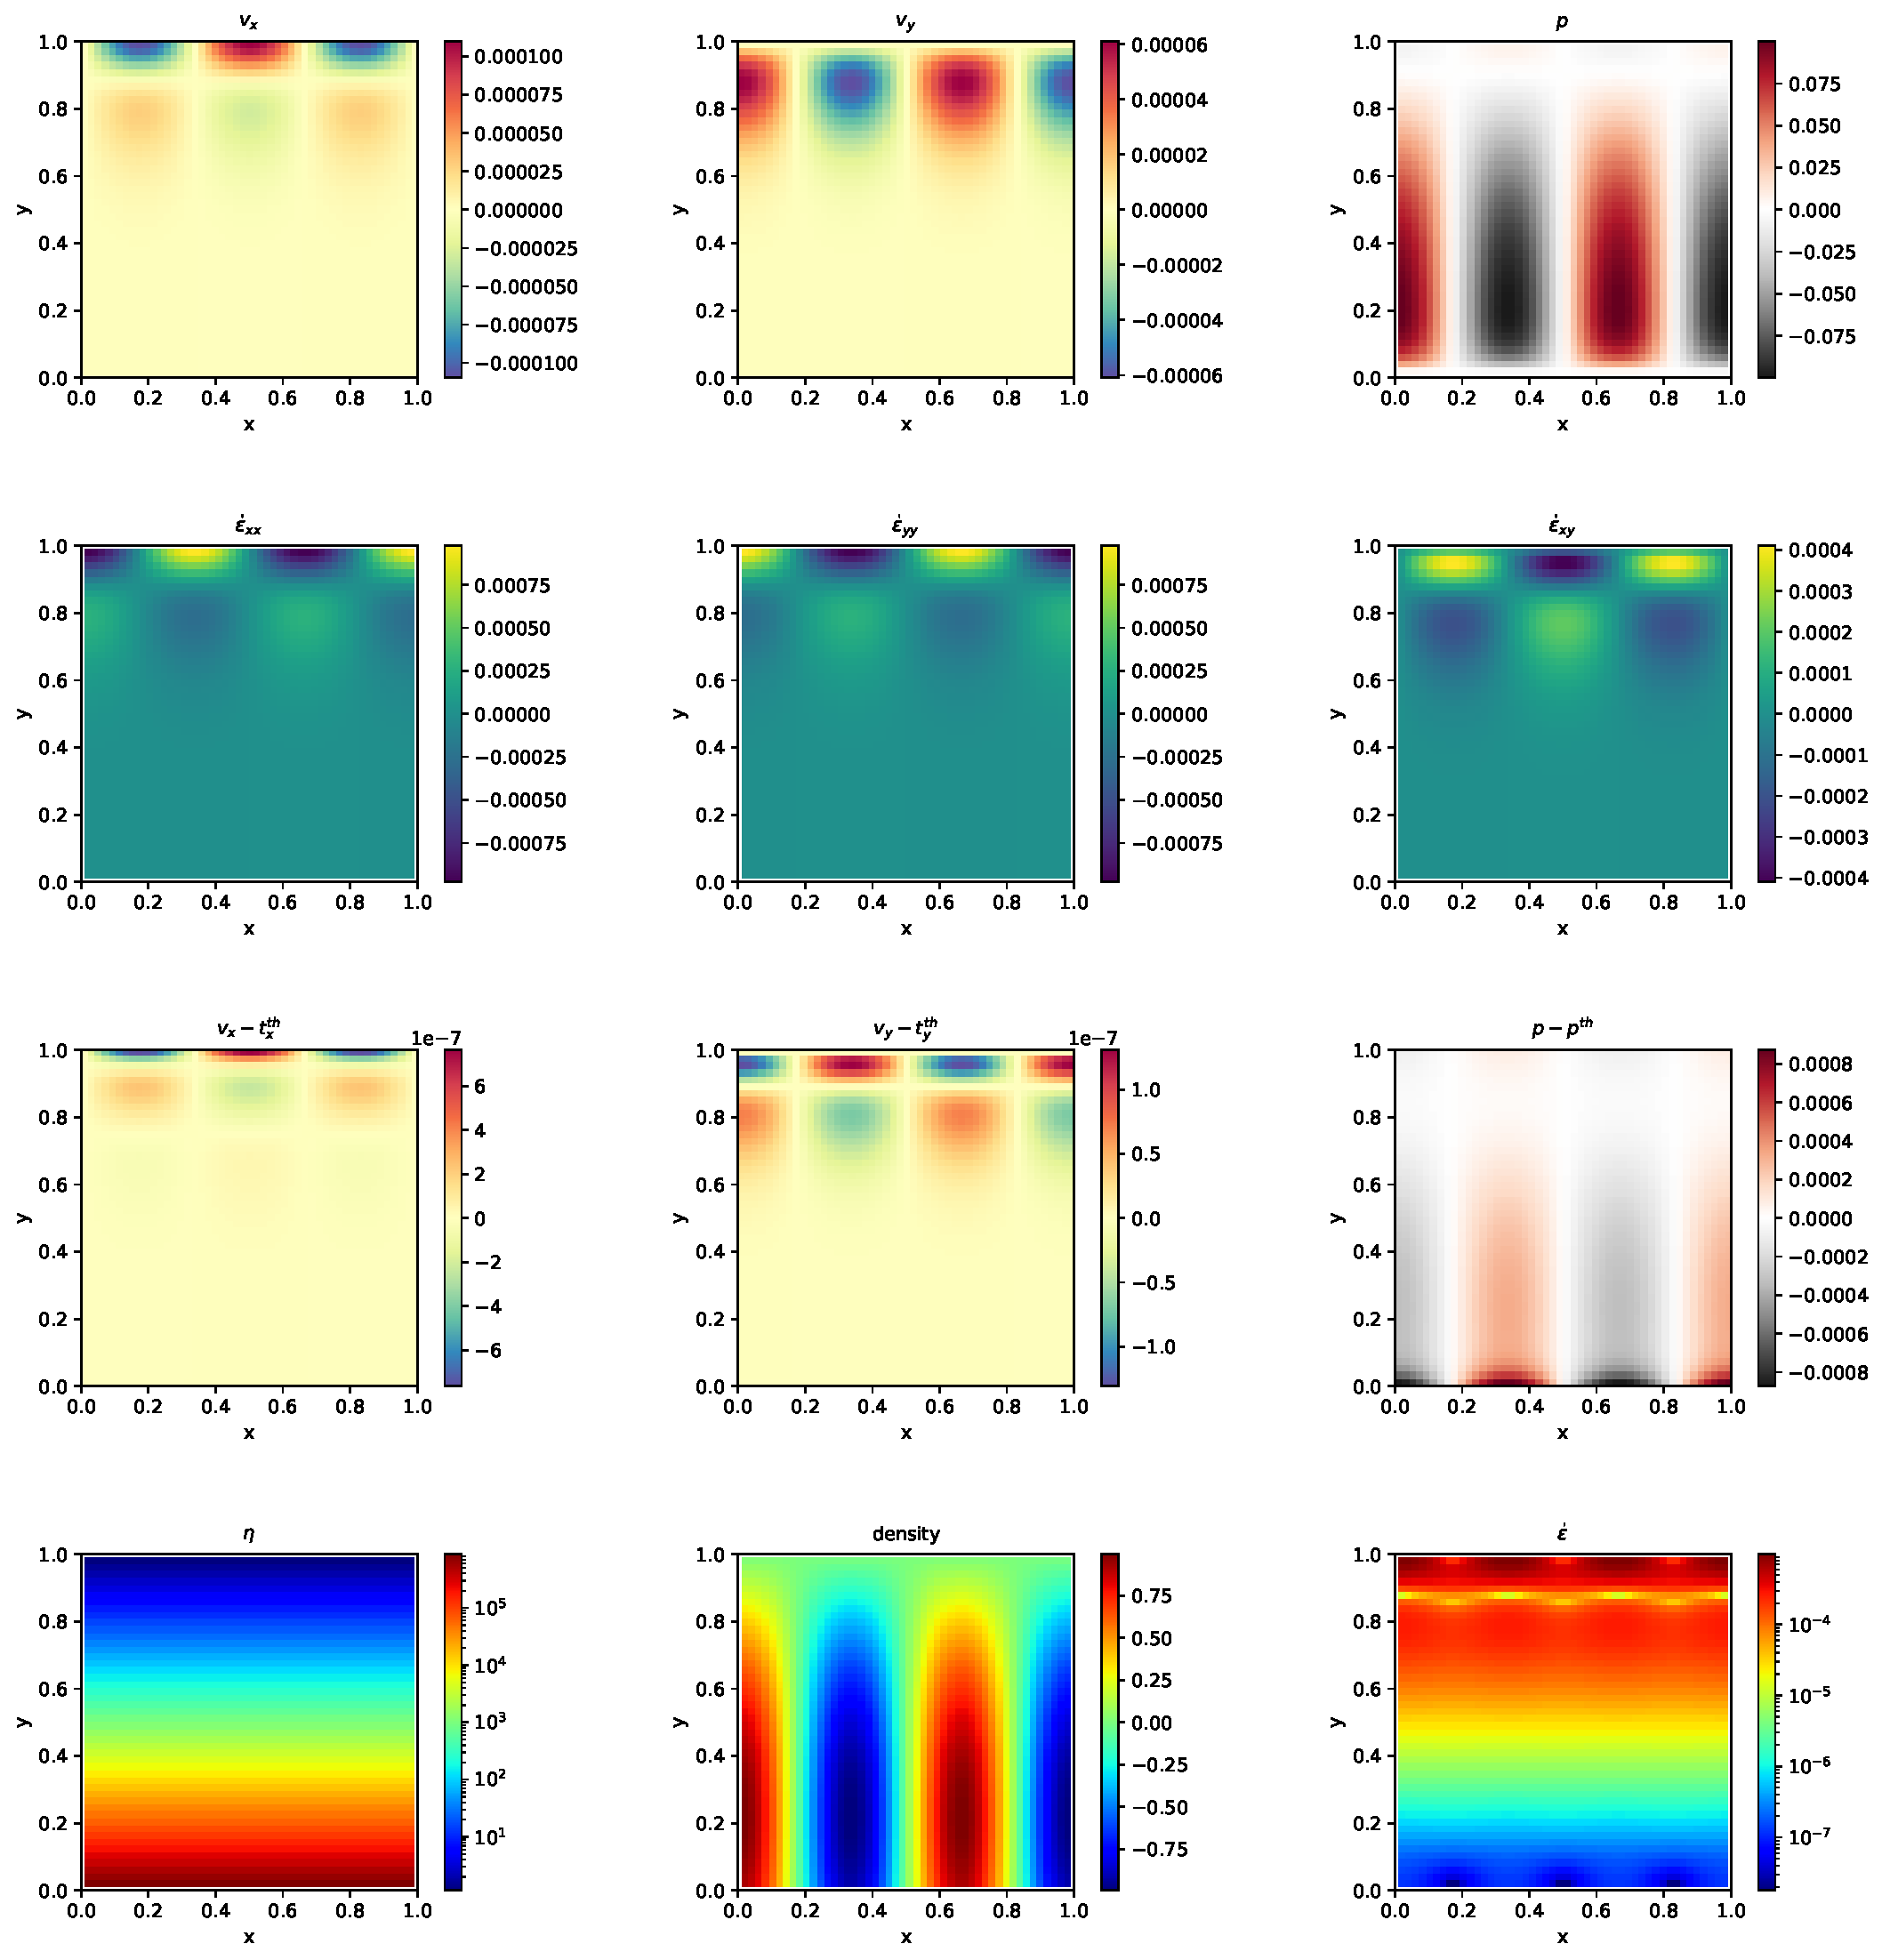
\includegraphics[width=12cm]{python_codes/fieldstone_solkz/solution.pdf}

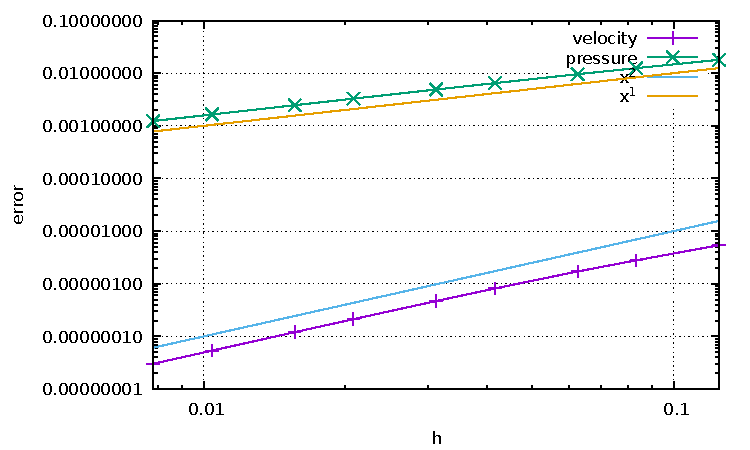
\includegraphics[width=8cm]{python_codes/fieldstone_solkz/errors.pdf}


\newpage
%%%%%%%%%%%%%%%%%%%%%%%%%%%%%%%%%%%%%%%%%%%%%%%%%%%%%%%%%%%%%%%%%%%%%%%%%%%%%%%
\section{{\tt fieldstone}: solvi benchmark}

Following SolCx and SolKz, the SolVi inclusion benchmark solves 
a problem with a discontinuous viscosity field, but in this case 
the viscosity field is chosen in such a way that the discontinuity 
is along a circle. Given the regular nature of the grid used by a majority of codes and the present one, 
this ensures that the discontinuity in the viscosity never aligns to cell boundaries.
This in turns leads to almost discontinuous pressures along the interface which are difficult to represent accurately.
\cite{scpo03} derived a simple analytic solution for the pressure and velocity fields for a circular 
inclusion under simple shear and it was used in \cite{deka08}, \cite{sunh10}, \cite{dumg11}, \cite{krhb12} and \cite{gemd13}.

Because of the symmetry of the problem, we only have to solve over the top right quarter of the domain (see Fig. \ref{fig_inclusion1}a). 

The analytical solution requires a strain rate boundary condition (e.g., pure shear) to be applied far away 
from the inclusion. In order to avoid using very large domains and/or dealing with this type of boundary condition altogether, 
the analytical solution is evaluated and imposed on the boundaries of the domain. 
By doing so, the truncation error introduced while discretizing the strain rate boundary condition is removed.

A characteristic of the analytic solution is that the pressure is zero inside the inclusion, while outside it follows the relation
\begin{equation}
p_m = 4 \dot{\epsilon}
\frac{\mu_m(\mu_i-\mu_m)}{\mu_i+\mu_m}
\frac{r_i^2}{r^2} \cos(2\theta)
\end{equation}
where $\mu_i = 10^3$ is the viscosity of the inclusion and $\mu_m = 1$ is the viscosity of the background media, $\theta=\tan^{-1}(y/x)$,
and $\dot{\epsilon}=1$ is the applied strain rate.

\cite{deka08} thoroughly investigated this problem with various numerical methods (FEM, FDM), with and without tracers, 
and conclusively showed how various averagings lead to different results. 
\cite{dumg11} obtained a first order convergence for both pressure and velocity, while \cite{krhb12}
and \cite{gemd13} showed that the use of adaptive mesh refinement in respectively the FEM and FDM 
yields convergence rates which depend on refinement strategies. 

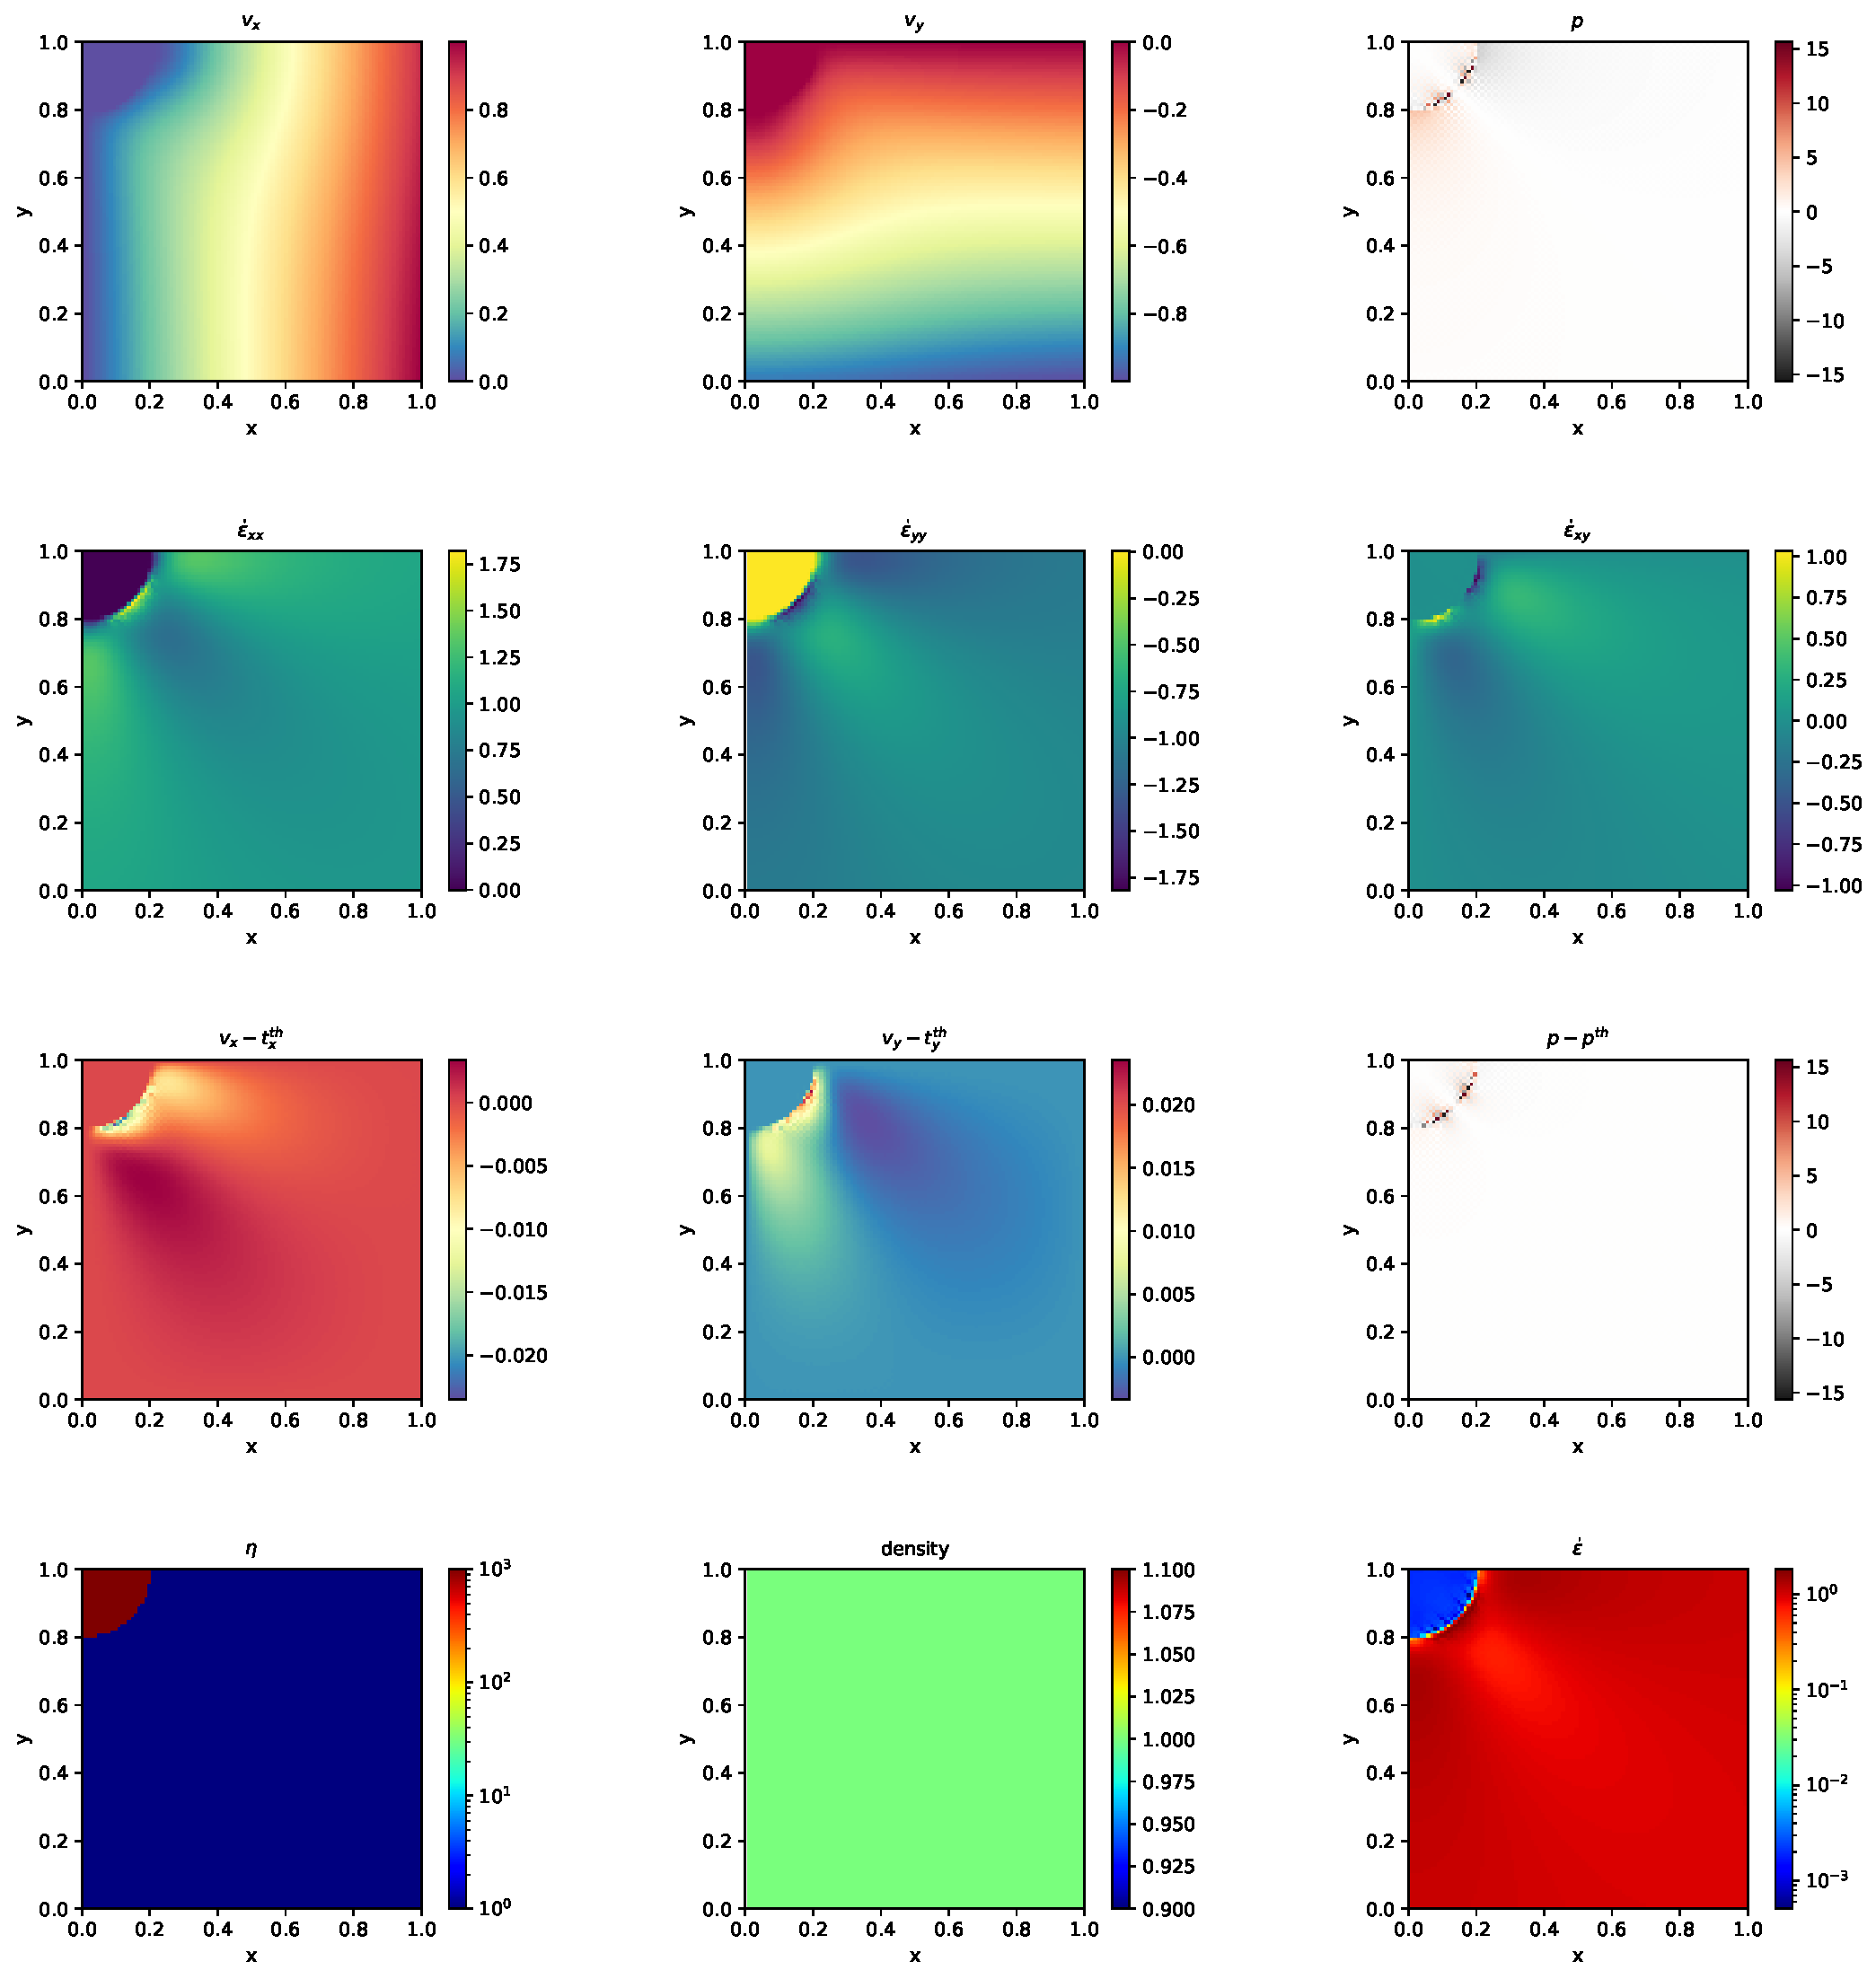
\includegraphics[width=15cm]{python_codes/fieldstone_solvi/solution}


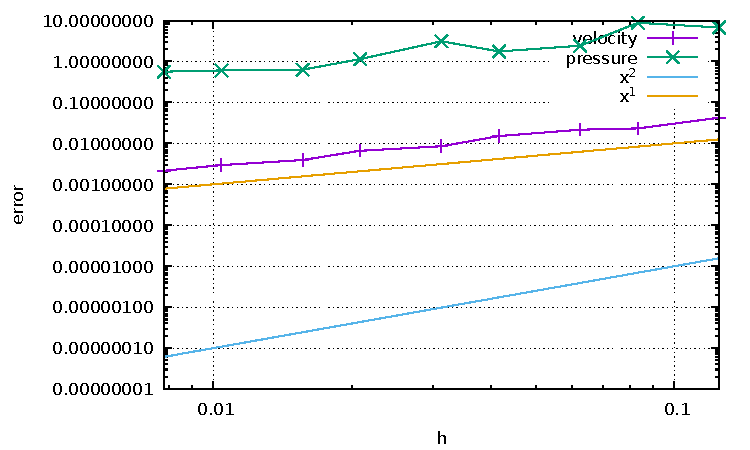
\includegraphics[width=8cm]{python_codes/fieldstone_solvi/errors}


\newpage
%%%%%%%%%%%%%%%%%%%%%%%%%%%%%%%%%%%%%%%%%%%%%%%%%%%%%%%%%%%%%%%%%%%%%%%%%%%%%%%
\section{{\tt fieldstone}: the indentor benchmark}

The punch benchmark is one of the few boundary value problems involving plastic solids for which there exists an exact solution. 
Such solutions are usually either for highly simplified geometries (spherical or axial symmetry, for instance) or simplified material models (such as rigid plastic solids) \cite{kacha04}.

In this experiment, a rigid punch indents a rigid plastic half space; the slip line field theory gives 
exact solutions as shown in Fig. \ref{fig_punch}a. 
The plane strain formulation of the equations and the detailed solution to the problem were derived in the Appendix of \cite{thfb08} and are also presented in \cite{gepd98}.

The two dimensional punch problem has been extensively studied numerically for the past 40 years 
\cite{zihl75,zihp95,chpe01,chan99,huhy99,yuti06,bufs08,raab07} and has been used to draw a parallel with the tectonics of eastern China in the context of the 
India-Eurasia collision \cite{tamo76,mota77}.
It is also worth noting that it has been carried out in one form or another in series of 
analogue modelling articles 
concerning the same region, with a rigid indenter colliding with a rheologically stratified lithosphere \cite{peta88,daco88,jodc90}.

 
Numerically, the one-time step punch experiment is performed on a two-dimensional
domain of purely plastic von Mises material. 
Given that the von Mises rheology yield criterion does not depend on pressure, the density of the material and/or the gravity vector is set to zero. Sides are set to free slip boundary conditions, the bottom to no slip, while a vertical velocity $(0,-v_p)$ is prescribed at the top boundary for nodes whose $x$ coordinate is within $[L_x/2-\delta/2,L_x/2+\delta/2]$. 

The following parameters are used: $L_x=1$, $L_y=0.5$, $\mu_{min}=10^{-3}$, 
$\mu_{max}=10^3$, $v_p=1$, $\delta=0.123456789$ 
and the yield value of the material is set to $k=1$. 

The analytical solution predicts that the angle of the shear bands stemming from the sides of the punch 
is $\pi/4$, that the pressure right under the punch is $1+\pi$, 
and that the velocity of the rigid blocks on each side of the punch is $v_p/\sqrt{2}$ 
(this is simply explained by invoking conservation of mass).

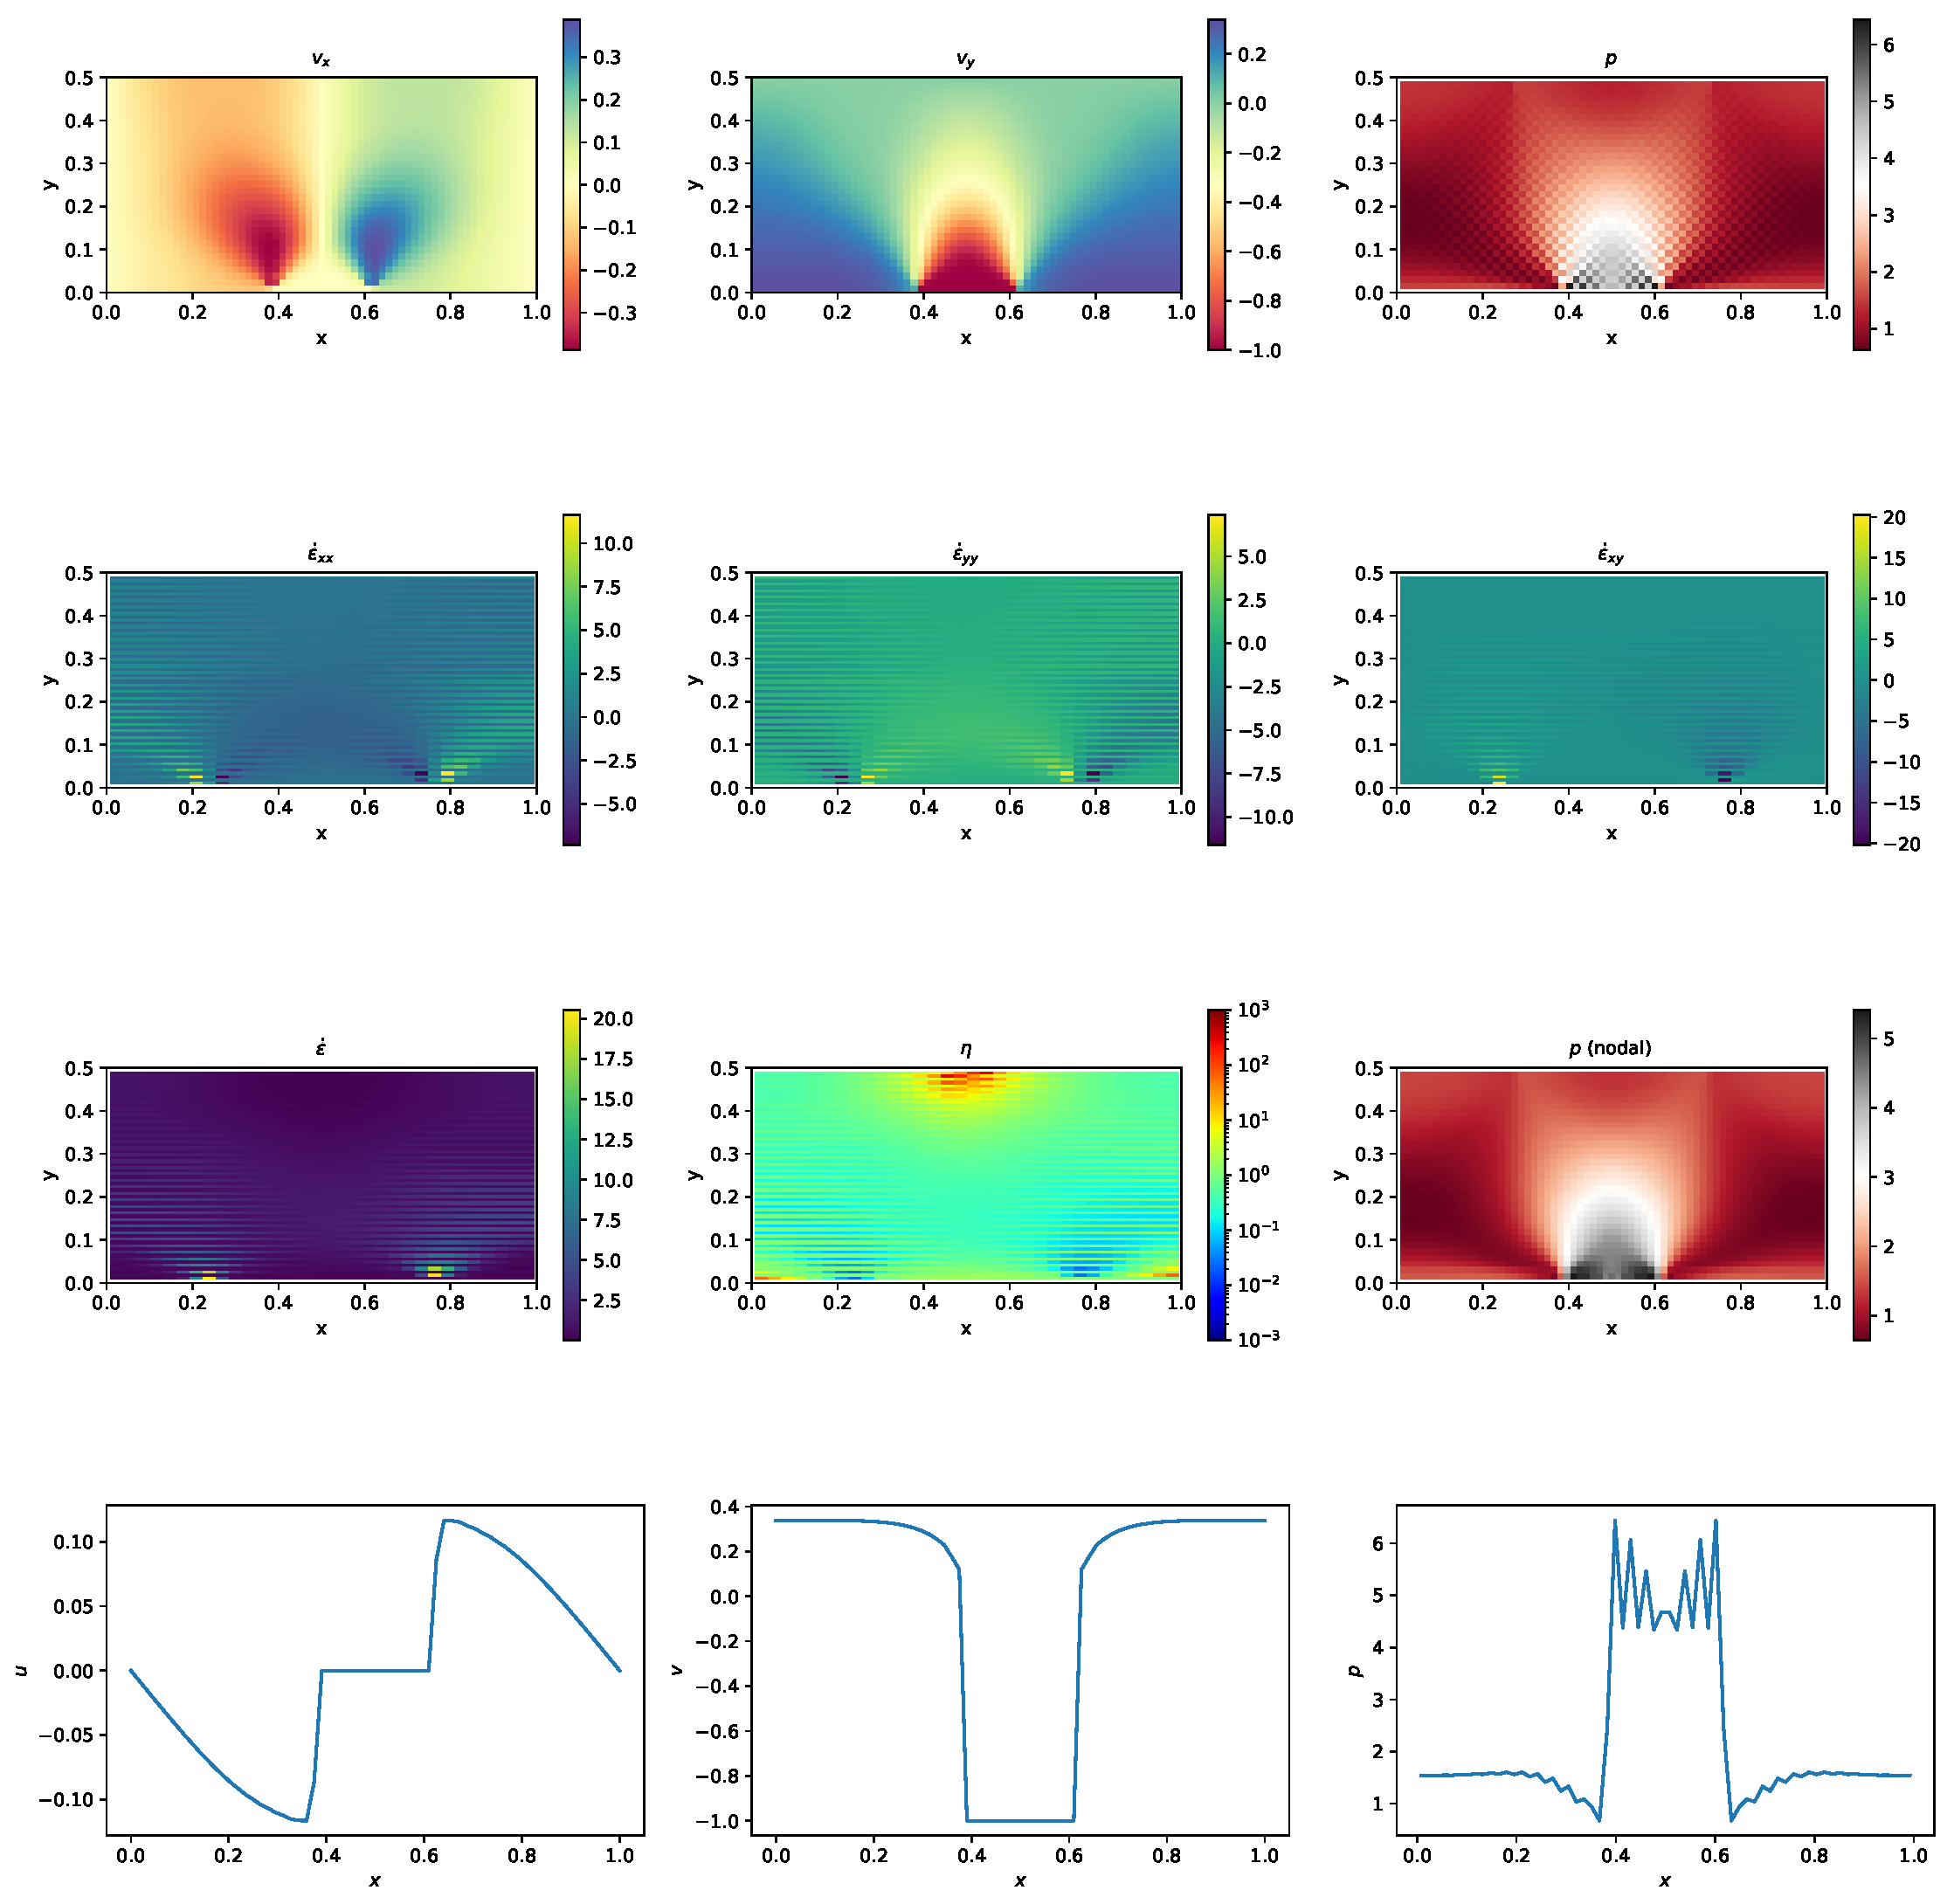
\includegraphics[width=16cm]{python_codes/fieldstone_indentor/solution.pdf}

ToDo: smooth punch

\fbox{
\parbox{10cm}{{\bf features}
\begin{itemize}
\item $Q_1\times P_0$ element \index{$Q_1 \times P_0$}
\item incompressible flow \index{incompressible flow}
\item penalty formulation \index{penalty formulation}
\item Dirichlet boundary conditions (no-slip)
\item isothermal \index{isothermal}
\item non-isoviscous \index{non-isoviscous}
\item nonlinear rheology \index{nonlinear rheology}
\end{itemize}
}}



\newpage
%%%%%%%%%%%%%%%%%%%%%%%%%%%%%%%%%%%%%%%%%%%%%%%%%%%%%%%%%%%%%%%%%%%%%%%%%%%%%%%
\section{{\tt fieldstone}: the annulus benchmark}
This benchmark is based on Thieulot \& Puckett [Subm.] in which an analytical solution to the
isoviscous incompressible Stokes equations is derived in an annulus geometry.
The velocity and pressure fields are as follows:

\begin{eqnarray}
v_r(r,\theta)     &=&  g(r) k \sin(k\theta), \\
v_\theta(r,\theta)&=&  f(r) \cos(k \theta), \\ 
p(r,\theta)       &=&  k h(r) \sin(k \theta), \\
\rho (r,\theta)   &=& \aleph(r) k \sin (k \theta), 
\end{eqnarray}
with
\begin{eqnarray}
f(r)&=&Ar+B/r, \\
g(r) &=& \frac{A}{2}r  +  \frac{B}{r} \ln r + \frac{C}{r}, \\
h(r)&=& \frac{2g(r)-f(r)}{r},  \\
\aleph(r) &=& g'' - \frac{g'}{r}  - \frac{g}{r^2} (k^2 - 1)  + \frac{f}{r^2}   + \frac{f'}{r}, \\
A &=& -C\frac{2(\ln R_1 - \ln R_2)} { R_2^2 \ln R_1  - R_1^2 \ln R_2}, \\
B &=& -C \frac{R_2^2-R_1^2}{R_2^2 \ln R_1 - R_1^2 \ln R_2}.
\end{eqnarray}

The parameters $A$ and $B$ are chosen so that $v_r(R_1)=v_r(R_2)=0$, i.e.
the velocity is tangential to both inner and outer surfaces.
The gravity vector is radial and of unit length.
In the present case, we set $R_1=1$, $R_2=2$ and $C=-1$. 

\fbox{
\parbox{10cm}{{\bf features}
\begin{itemize}
\item $Q_1\times P_0$ element
\item incompressible flow
\item penalty formulation
\item Dirichlet boundary conditions
\item direct solver
\item isothermal
\item isoviscous
\item analytical solution
\item annulus geometry
\item elemental boundary conditions
\end{itemize}
}}

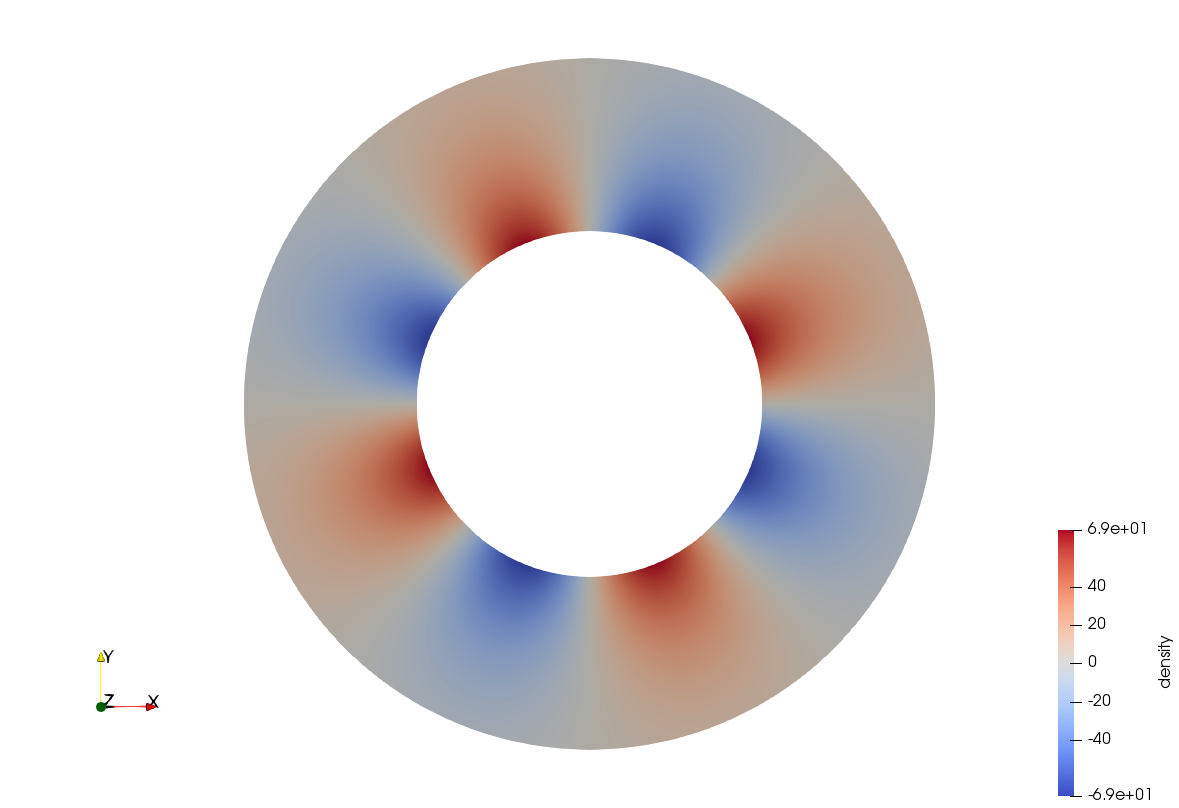
\includegraphics[width=6cm]{python_codes/fieldstone_annulus/density}
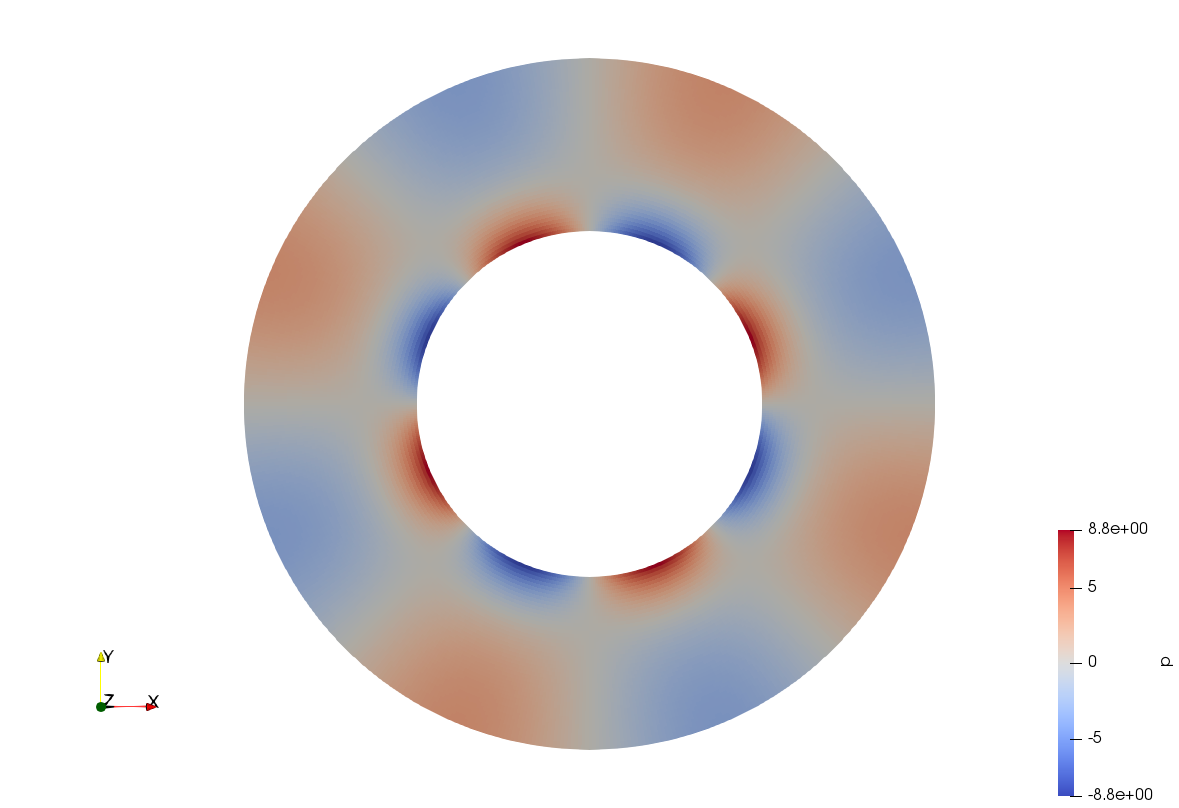
\includegraphics[width=6cm]{python_codes/fieldstone_annulus/pressure}
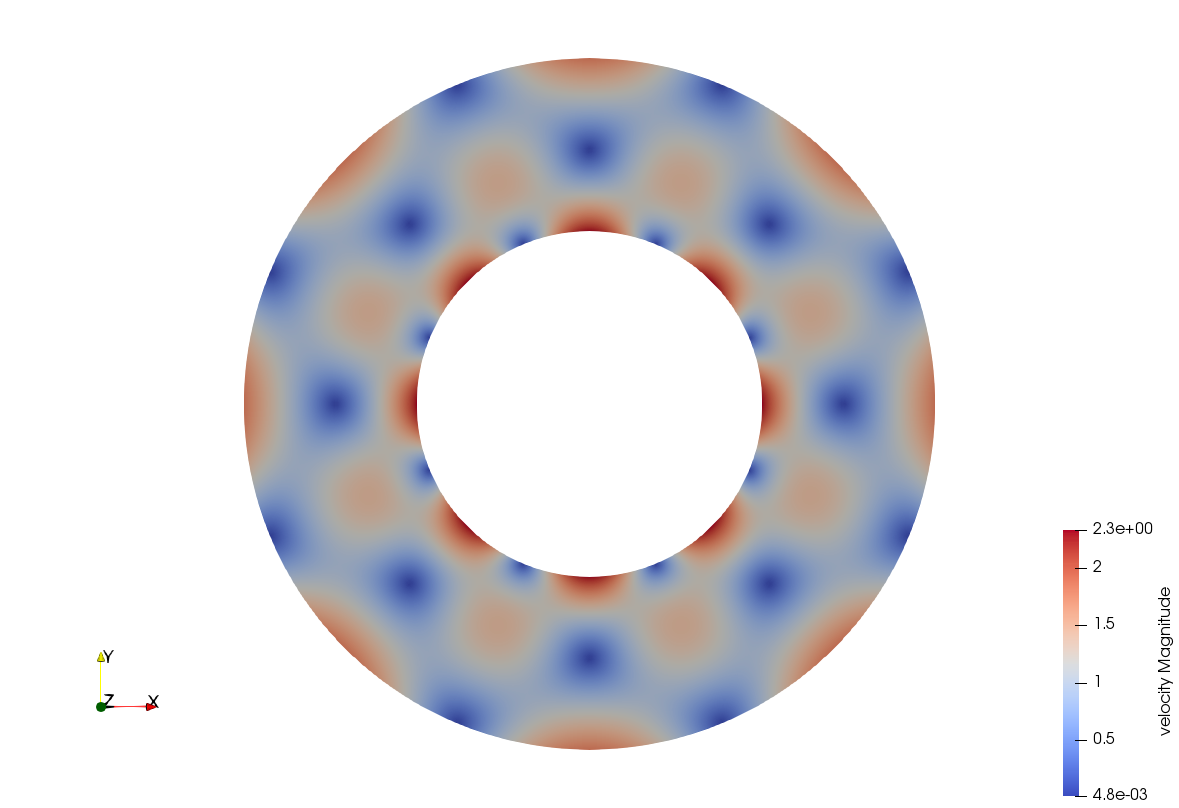
\includegraphics[width=6cm]{python_codes/fieldstone_annulus/velocity}

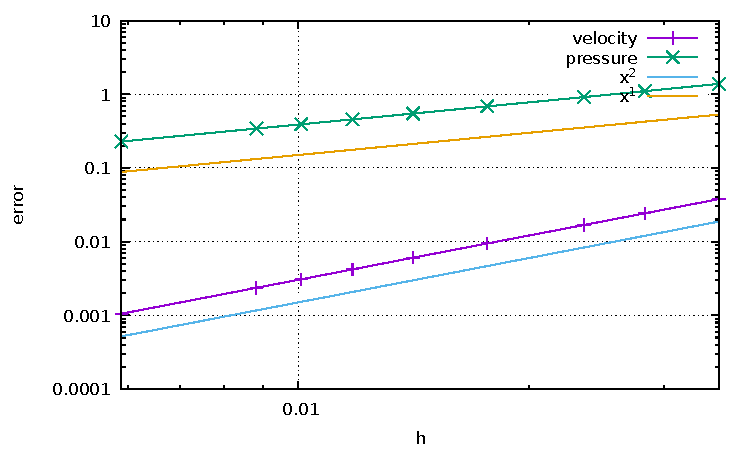
\includegraphics[width=16cm]{python_codes/fieldstone_annulus/errors}




\newpage
%%%%%%%%%%%%%%%%%%%%%%%%%%%%%%%%%%%%%%%%%%%%%%%%%%%%%%%%%%%%%%%%%%%%%%%%%%%%%%%
\section{{\tt fieldstone}: stokes sphere (3D) - penalty\label{f5}}

\fbox{
\parbox{10cm}{{\bf features}
\begin{itemize}
\item $Q_1\times P_0$ element
\item incompressible flow
\item penalty formulation
\item Dirichlet boundary conditions (free-slip)
\item direct solver
\item isothermal
\item non-isoviscous
\item 3D
\item elemental b.c. 
\item buoyancy driven
\end{itemize}
}}


\begin{center}
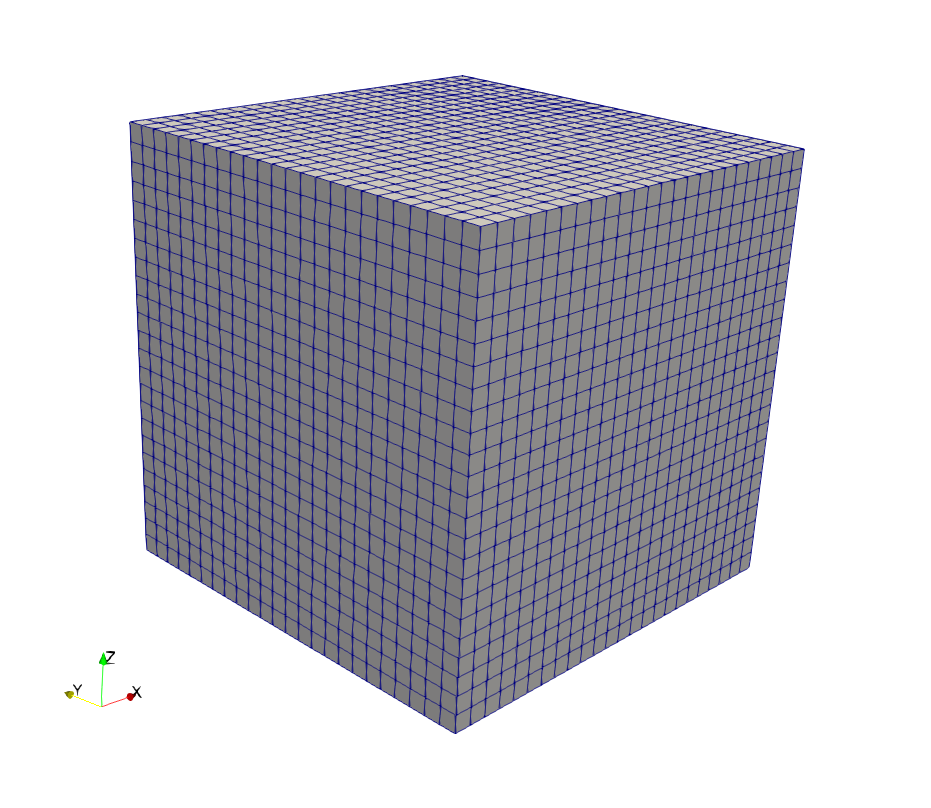
\includegraphics[width=5cm]{python_codes/fieldstone_stokes_sphere_3D/grid}
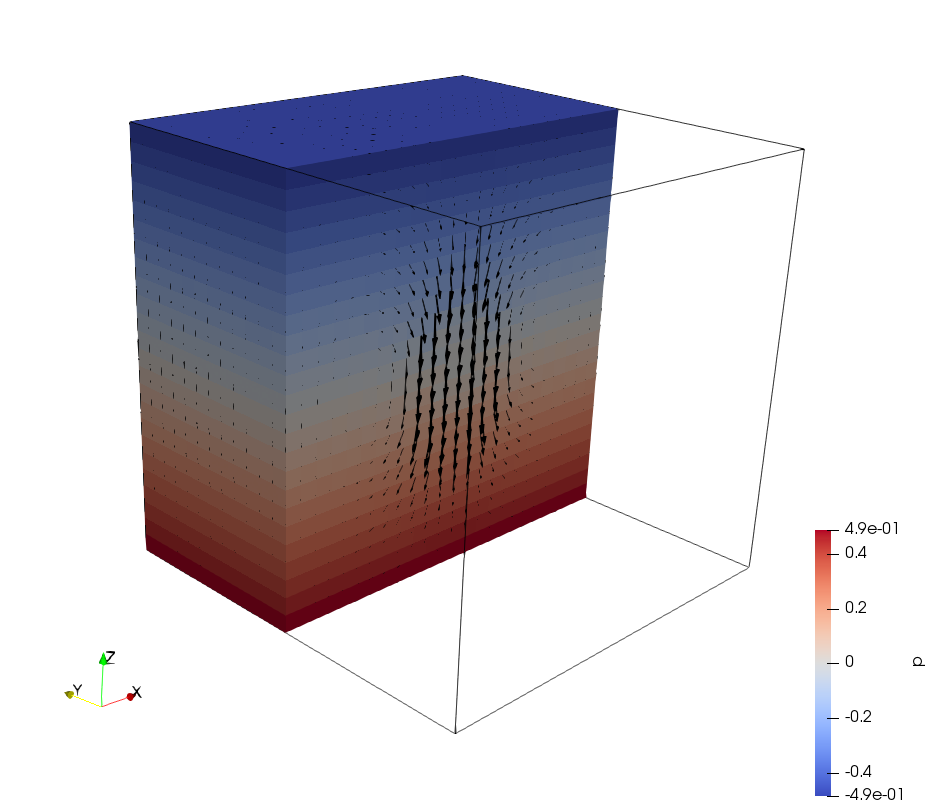
\includegraphics[width=5cm]{python_codes/fieldstone_stokes_sphere_3D/vel}
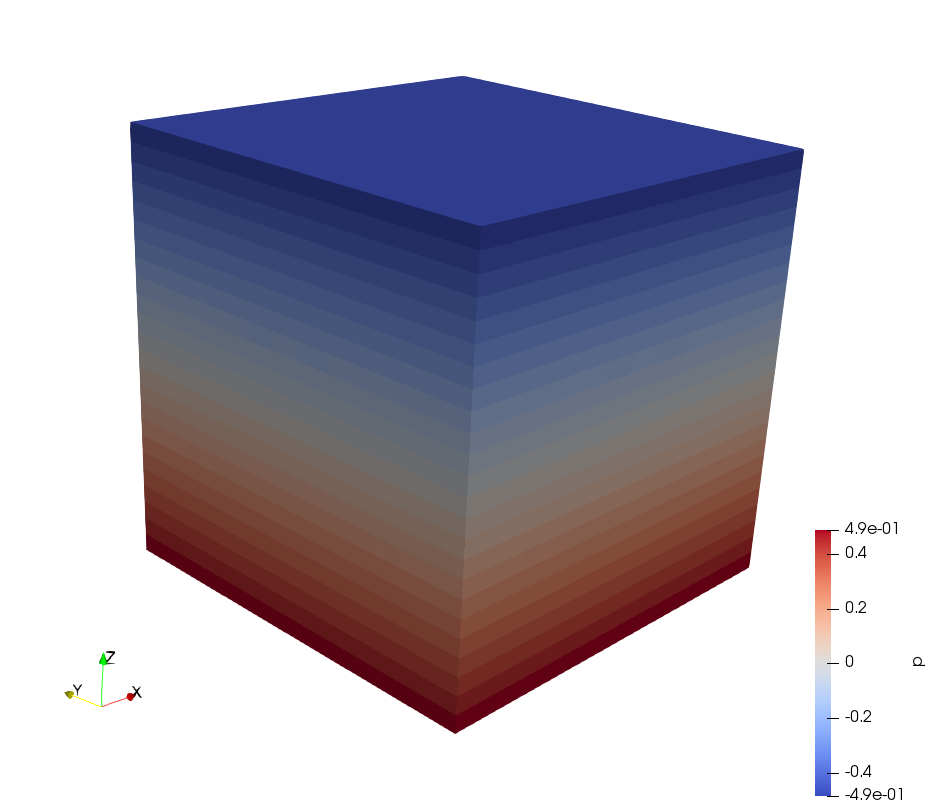
\includegraphics[width=5cm]{python_codes/fieldstone_stokes_sphere_3D/press}\\
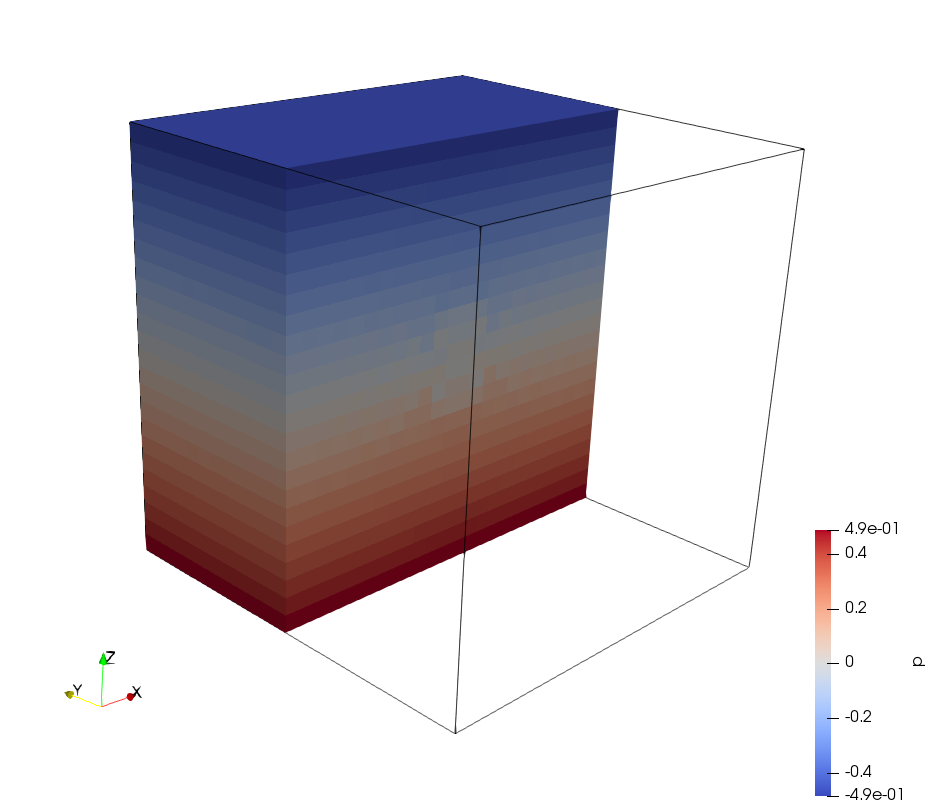
\includegraphics[width=5cm]{python_codes/fieldstone_stokes_sphere_3D/press2}
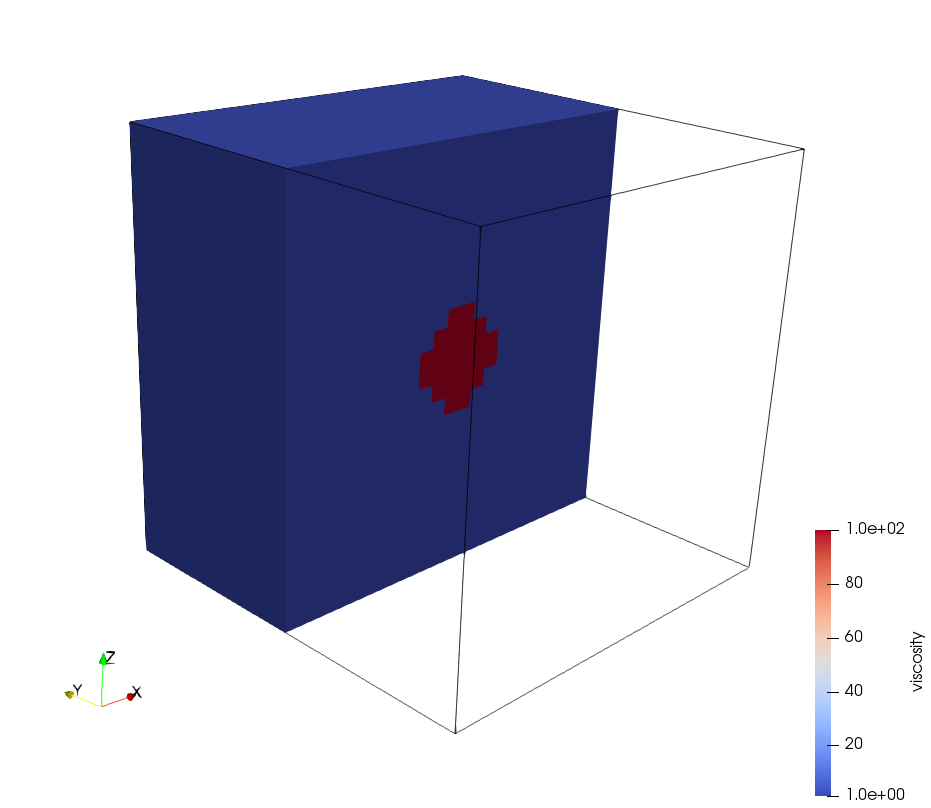
\includegraphics[width=5cm]{python_codes/fieldstone_stokes_sphere_3D/visc}
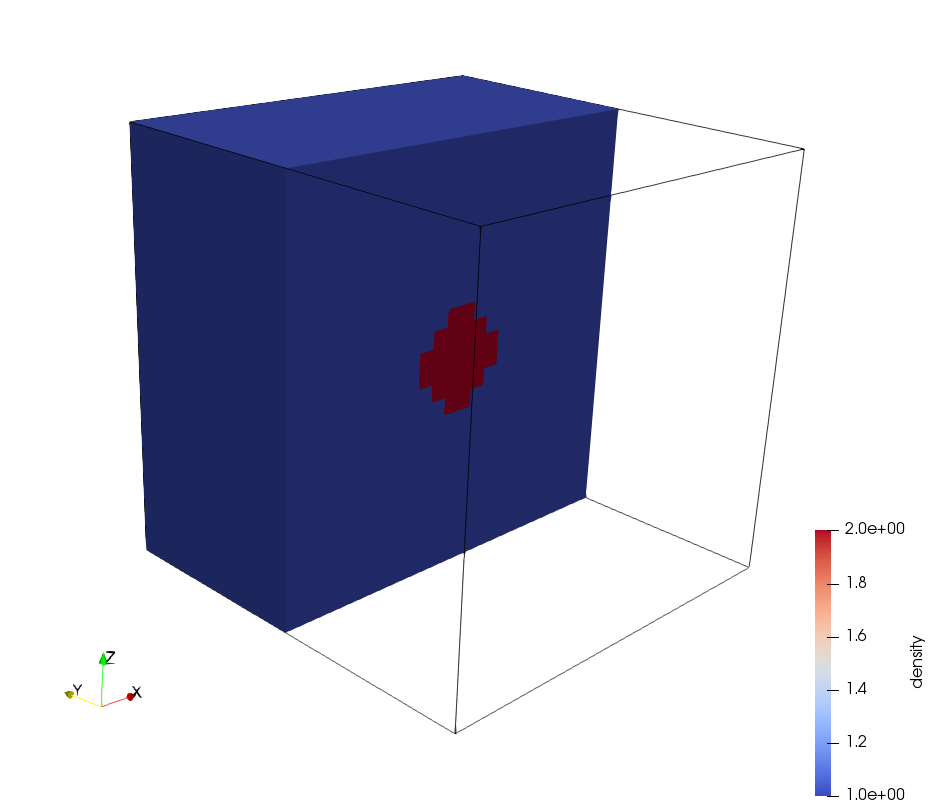
\includegraphics[width=5cm]{python_codes/fieldstone_stokes_sphere_3D/dens}\\
{\small resolution is 24x24x24}
\end{center}



\newpage
%%%%%%%%%%%%%%%%%%%%%%%%%%%%%%%%%%%%%%%%%%%%%%%%%%%%%%%%%%%%%%%%%%%%%%%%%%%%%%%
\section{{\tt fieldstone}: stokes sphere (3D) - mixed formulation\label{f5}}

This is the same setup as Section \ref{f5}.

\fbox{
\parbox{10cm}{{\bf features}
\begin{itemize}
\item $Q_1\times P_0$ element
\item incompressible flow
\item mixed formulation
\item Dirichlet boundary conditions (free-slip)
\item direct solver
\item isothermal
\item non-isoviscous
\item 3D
\item elemental b.c. 
\item buoyancy driven
\end{itemize}
}}



\newpage
%%%%%%%%%%%%%%%%%%%%%%%%%%%%%%%%%%%%%%%%%%%%%%%%%%%%%%%%%%%%%%%%%%%%%%%%%%%%%%%
\section{{\tt fieldstone}: consistent pressure recovery }
What follows is presented in \cite{zina82}. The second part of their paper wishes to establish a simple
and effective numerical method to calculate variables eliminated by the penalisation process. 
The method involves an additional finite element solution for the nodal pressures using 
the same finite element basis and numerical quadrature as used for the velocity.

Let us start with:
\[
p = -\lambda {\bm \nabla}\cdot {\bm v}
\]
which lead to
\[
(q,p)=-\lambda (q,{\bm \nabla}\cdot{\bm v})
\]
and then
\[
\left( \int {\bm N} {\bm N} d\Omega \right) \cdot {\bm P} = - \left( \lambda \int {\bm N} {\bm \nabla}{\bm N} d\Omega \right)\cdot{\bm V}
\]
or, 
\[
{\bm M} \cdot {\bm P} = - {\bm D}\cdot{\bm V}
\]
and finally
\[
{\bm P} = -{\bm M}^{-1} \cdot {\bm D} \cdot {V}
\]
with ${\bm M}$ of size $(np\times np)$, ${\bm D}$ of size $(np*ndof\times np*ndof)$ and ${\bm V}$ of size $(np*ndof)$.
The vector ${\bm P}$ contains the $np$ nodal pressure values directly, with no need for a smoothing scheme. 
The mass matrix ${\bm M}$ is to be evaluated at the full integration points, while the constraint part (the right
hand side of the equation) is to be evaluated at the reduced integration point. 

As noted by \cite{zina82}, it is interesting to note that when linear elements are used and the lumped matrices
are used for the ${\bm M}$ the resulting algebraic equation is identical to the smoothing scheme based
on the averaging method only if the uniform square finite element mesh is used. 
In this respect this method is expected to yield different results when elements are not square or even rectangular.

-------

$q_1$ is smoothed pressure obtained with the  center-to-node approach.

$q_2$ is recovered pressure obtained with \cite{zina82}.

All three fulfill the zero average condition: $\int p d\Omega = 0$.

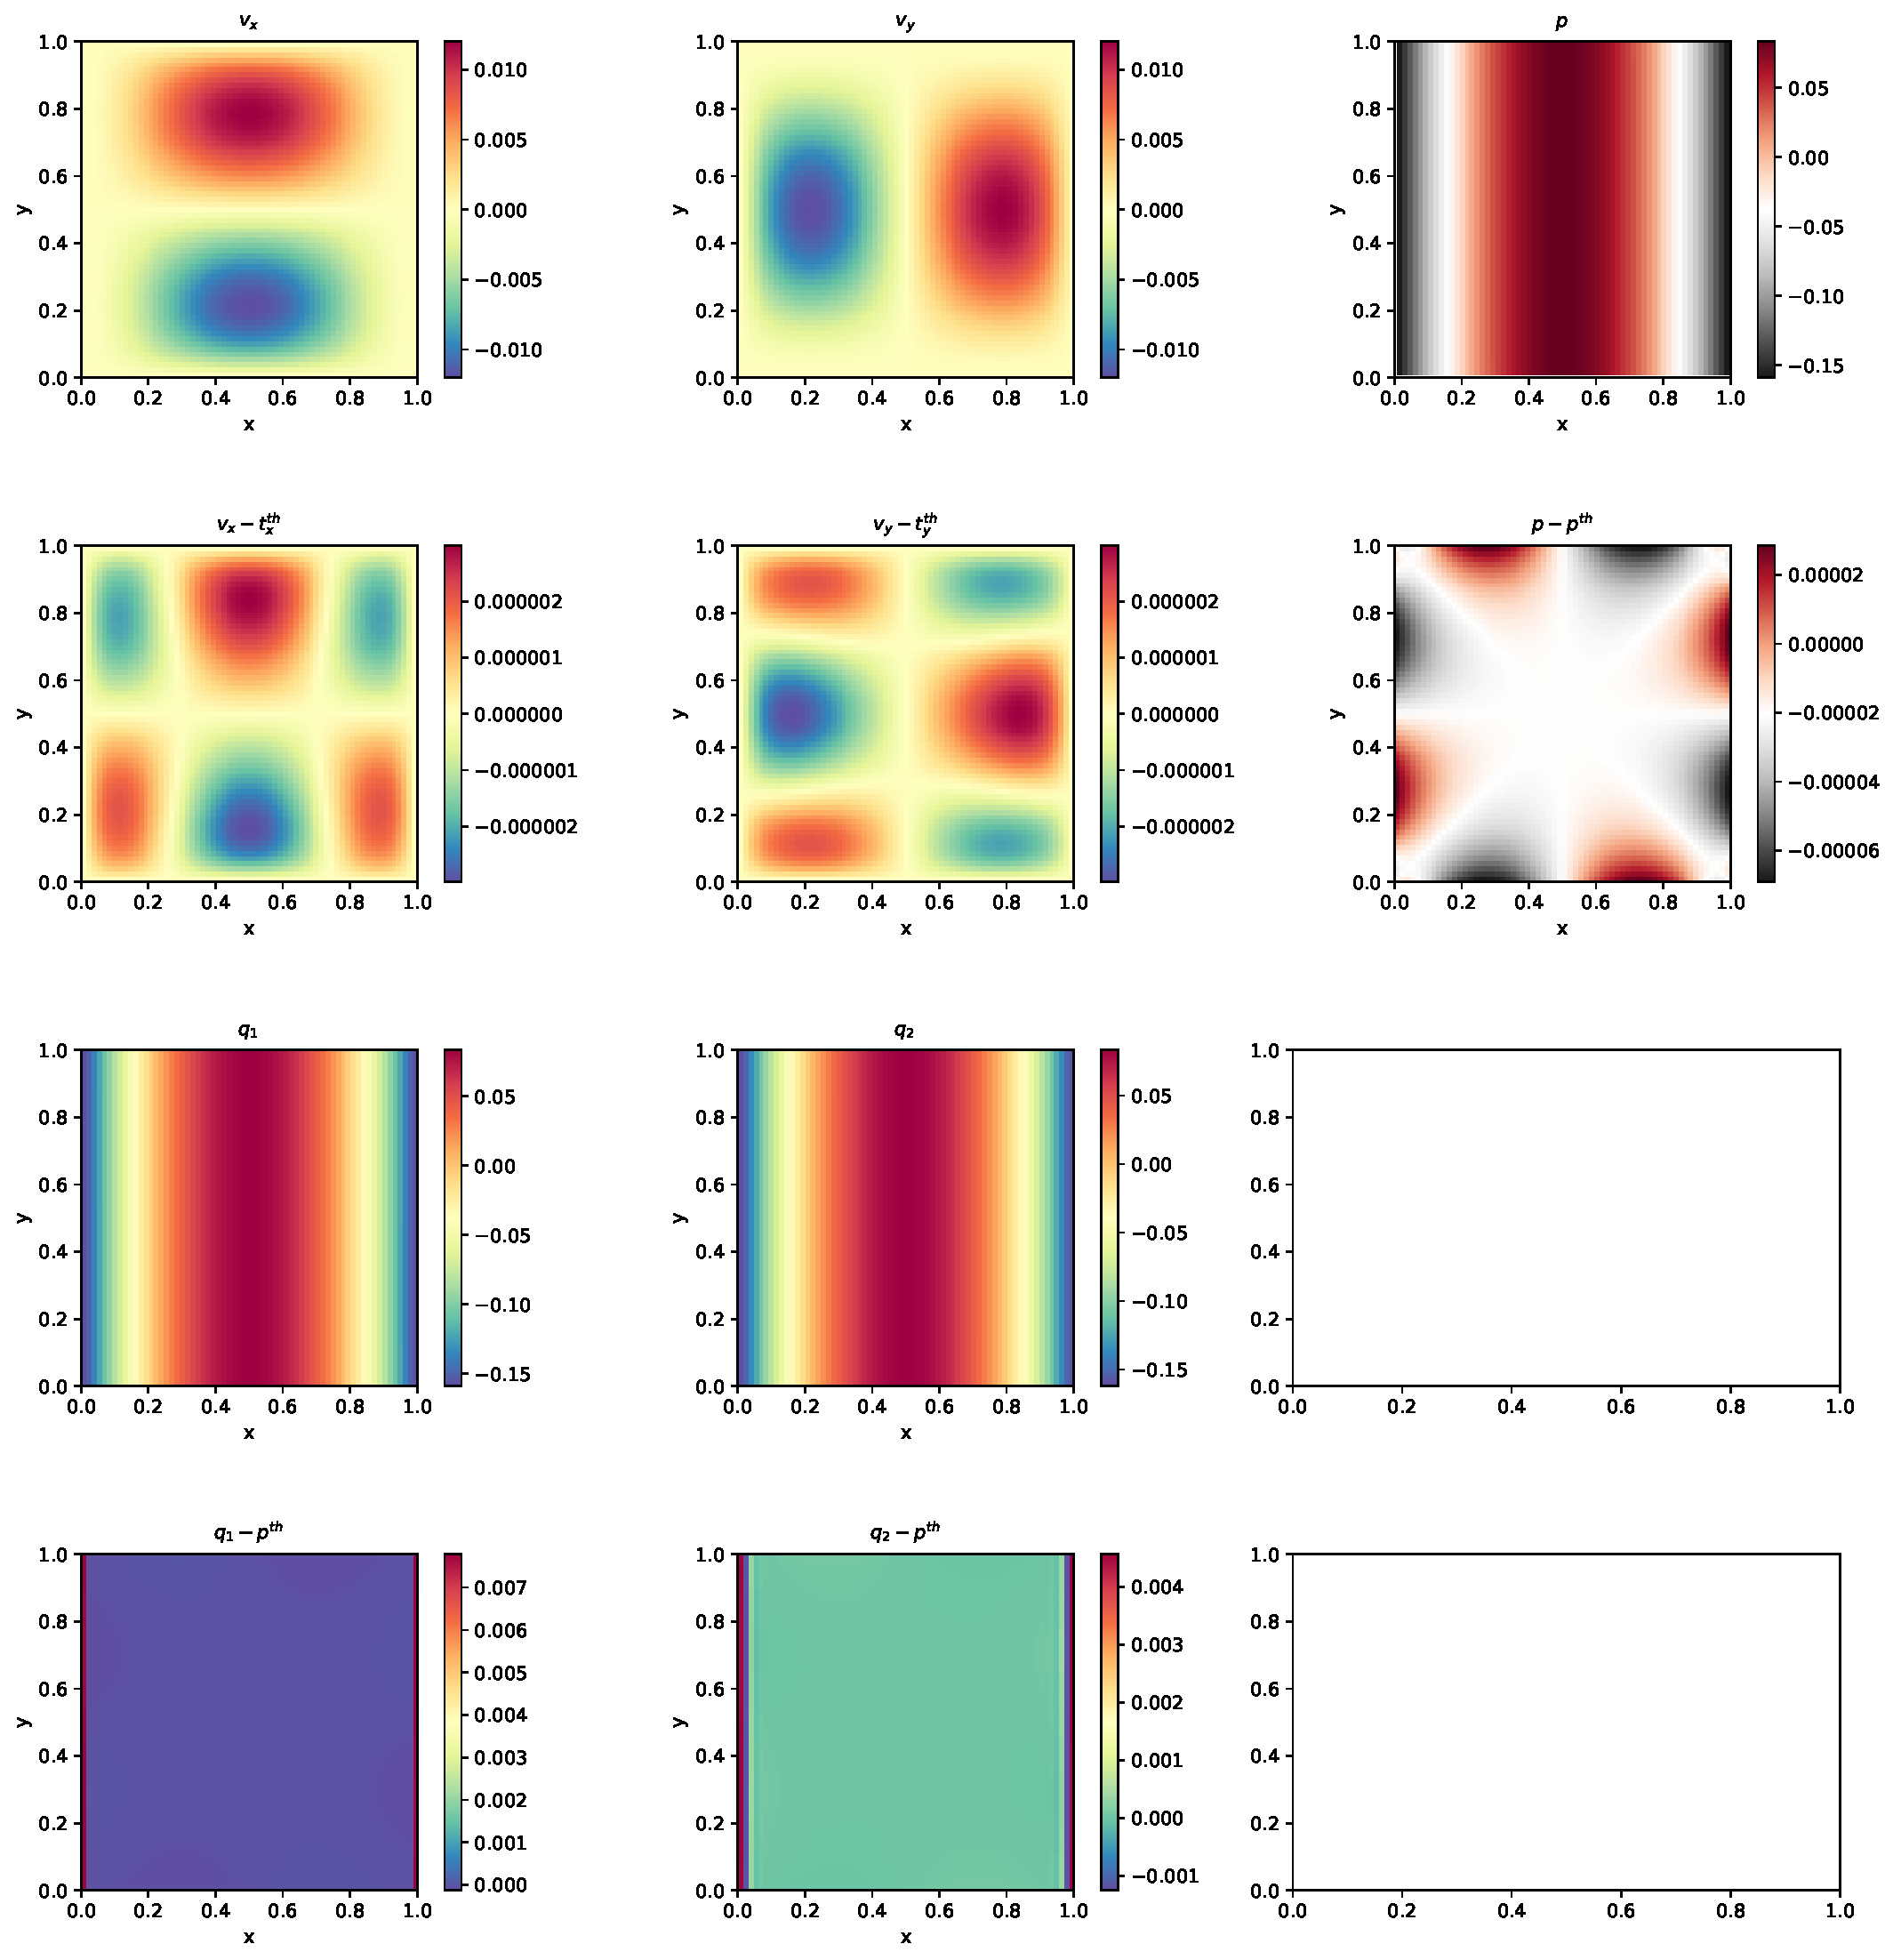
\includegraphics[width=15cm]{python_codes/fieldstone_consistent_pressure_recovery/solution}

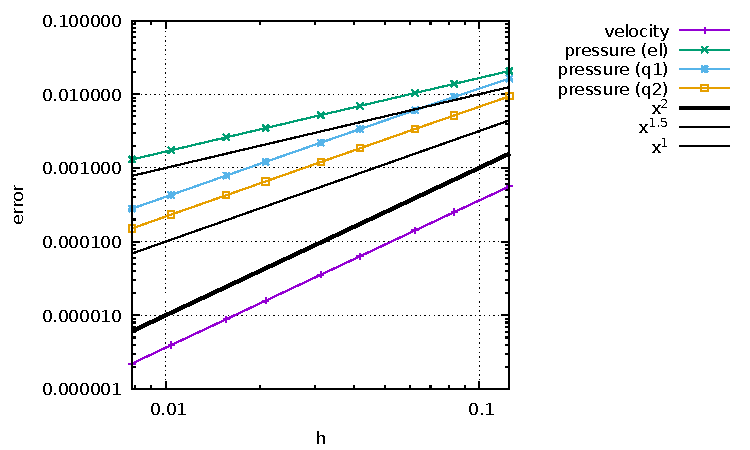
\includegraphics[width=8cm]{python_codes/fieldstone_consistent_pressure_recovery/errors}

In terms of pressure error, $q_2$ is better than $q_1$ which is better than elemental.

QUESTION: why are the averages exactly zero ?!

TODO: 
\begin{itemize}
\item add randomness to internal node positions.
\item look at elefant algorithms
\end{itemize}


\newpage
%%%%%%%%%%%%%%%%%%%%%%%%%%%%%%%%%%%%%%%%%%%%%%%%%%%%%%%%%%%%%%%%%%%%%%%%%%%%%%%
\section{{\tt fieldstone}: the Particle in Cell technique (1) - the effect of averaging}



\newpage
%%%%%%%%%%%%%%%%%%%%%%%%%%%%%%%%%%%%%%%%%%%%%%%%%%%%%%%%%%%%%%%%%%%%%%%%%%%%%%%
\section{{\tt fieldstone}: solving the full saddle point problem}
The details of the numerical setup are presented in Section \ref{f1}.

The main difference is that we no longer use the penalty formulation and therefore 
keep both velocity and pressure as unknowns. Therefore we end up having to solve 
the following system:
\[
\left(
\begin{array}{cc}
\K & \G \\ \G^T & 0 
\end{array}
\right)
\cdot
\left(
\begin{array}{c}
V \\ P
\end{array}
\right)
=
\left(
\begin{array}{c}
 f \\ h
\end{array}
\right)
\quad\quad
{\rm or,}
\quad\quad
\A \cdot X = rhs
\]
Each block $\K$, $\G$ and vector $f$, $h$ are built separately in the code and assembled into 
the matrix $\A$ and vector $rhs$ afterwards. $\A$ and $rhs$ are then passed to the solver. 
We will see later that there are alternatives to solve this approach which do not require to 
build the full Stokes matrix $\A$. 

Each element has $m=4$ vertices so in total $ndofV\times m=8$ velocity dofs and a single 
pressure dof, commonly situated in the center of the element. The total number of 
velocity dofs is therefore $NfemV=nnp \times ndofV$ while the total number of
pressure dofs is $NfemP=nel$. The total number of dofs is then $Nfem=NfemV+NfemP$.

As a consequence, matrix $\K$ has size $NfemV,NfemV$ and matrix $\G$ has size $NfemV,NfemP$.
Vector $f$ is of size $NfemV$ and vector $h$ is of size $NfemP$.  


\fbox{
\parbox{10cm}{{\bf features}
\begin{itemize}
\item $Q_1\times P_0$ element \index{$Q_1 \times P_0$}
\item incompressible flow \index{incompressible flow}
\item mixed formulation \index{mixed formulation}
\item Dirichlet boundary conditions (no-slip)
\item direct solver (?)
\item isothermal \index{isothermal}
\item isoviscous \index{isoviscous}
\item analytical solution \index{analytical solution}
\item pressure smoothing \index{pressure smoothing} 
\end{itemize}
}}

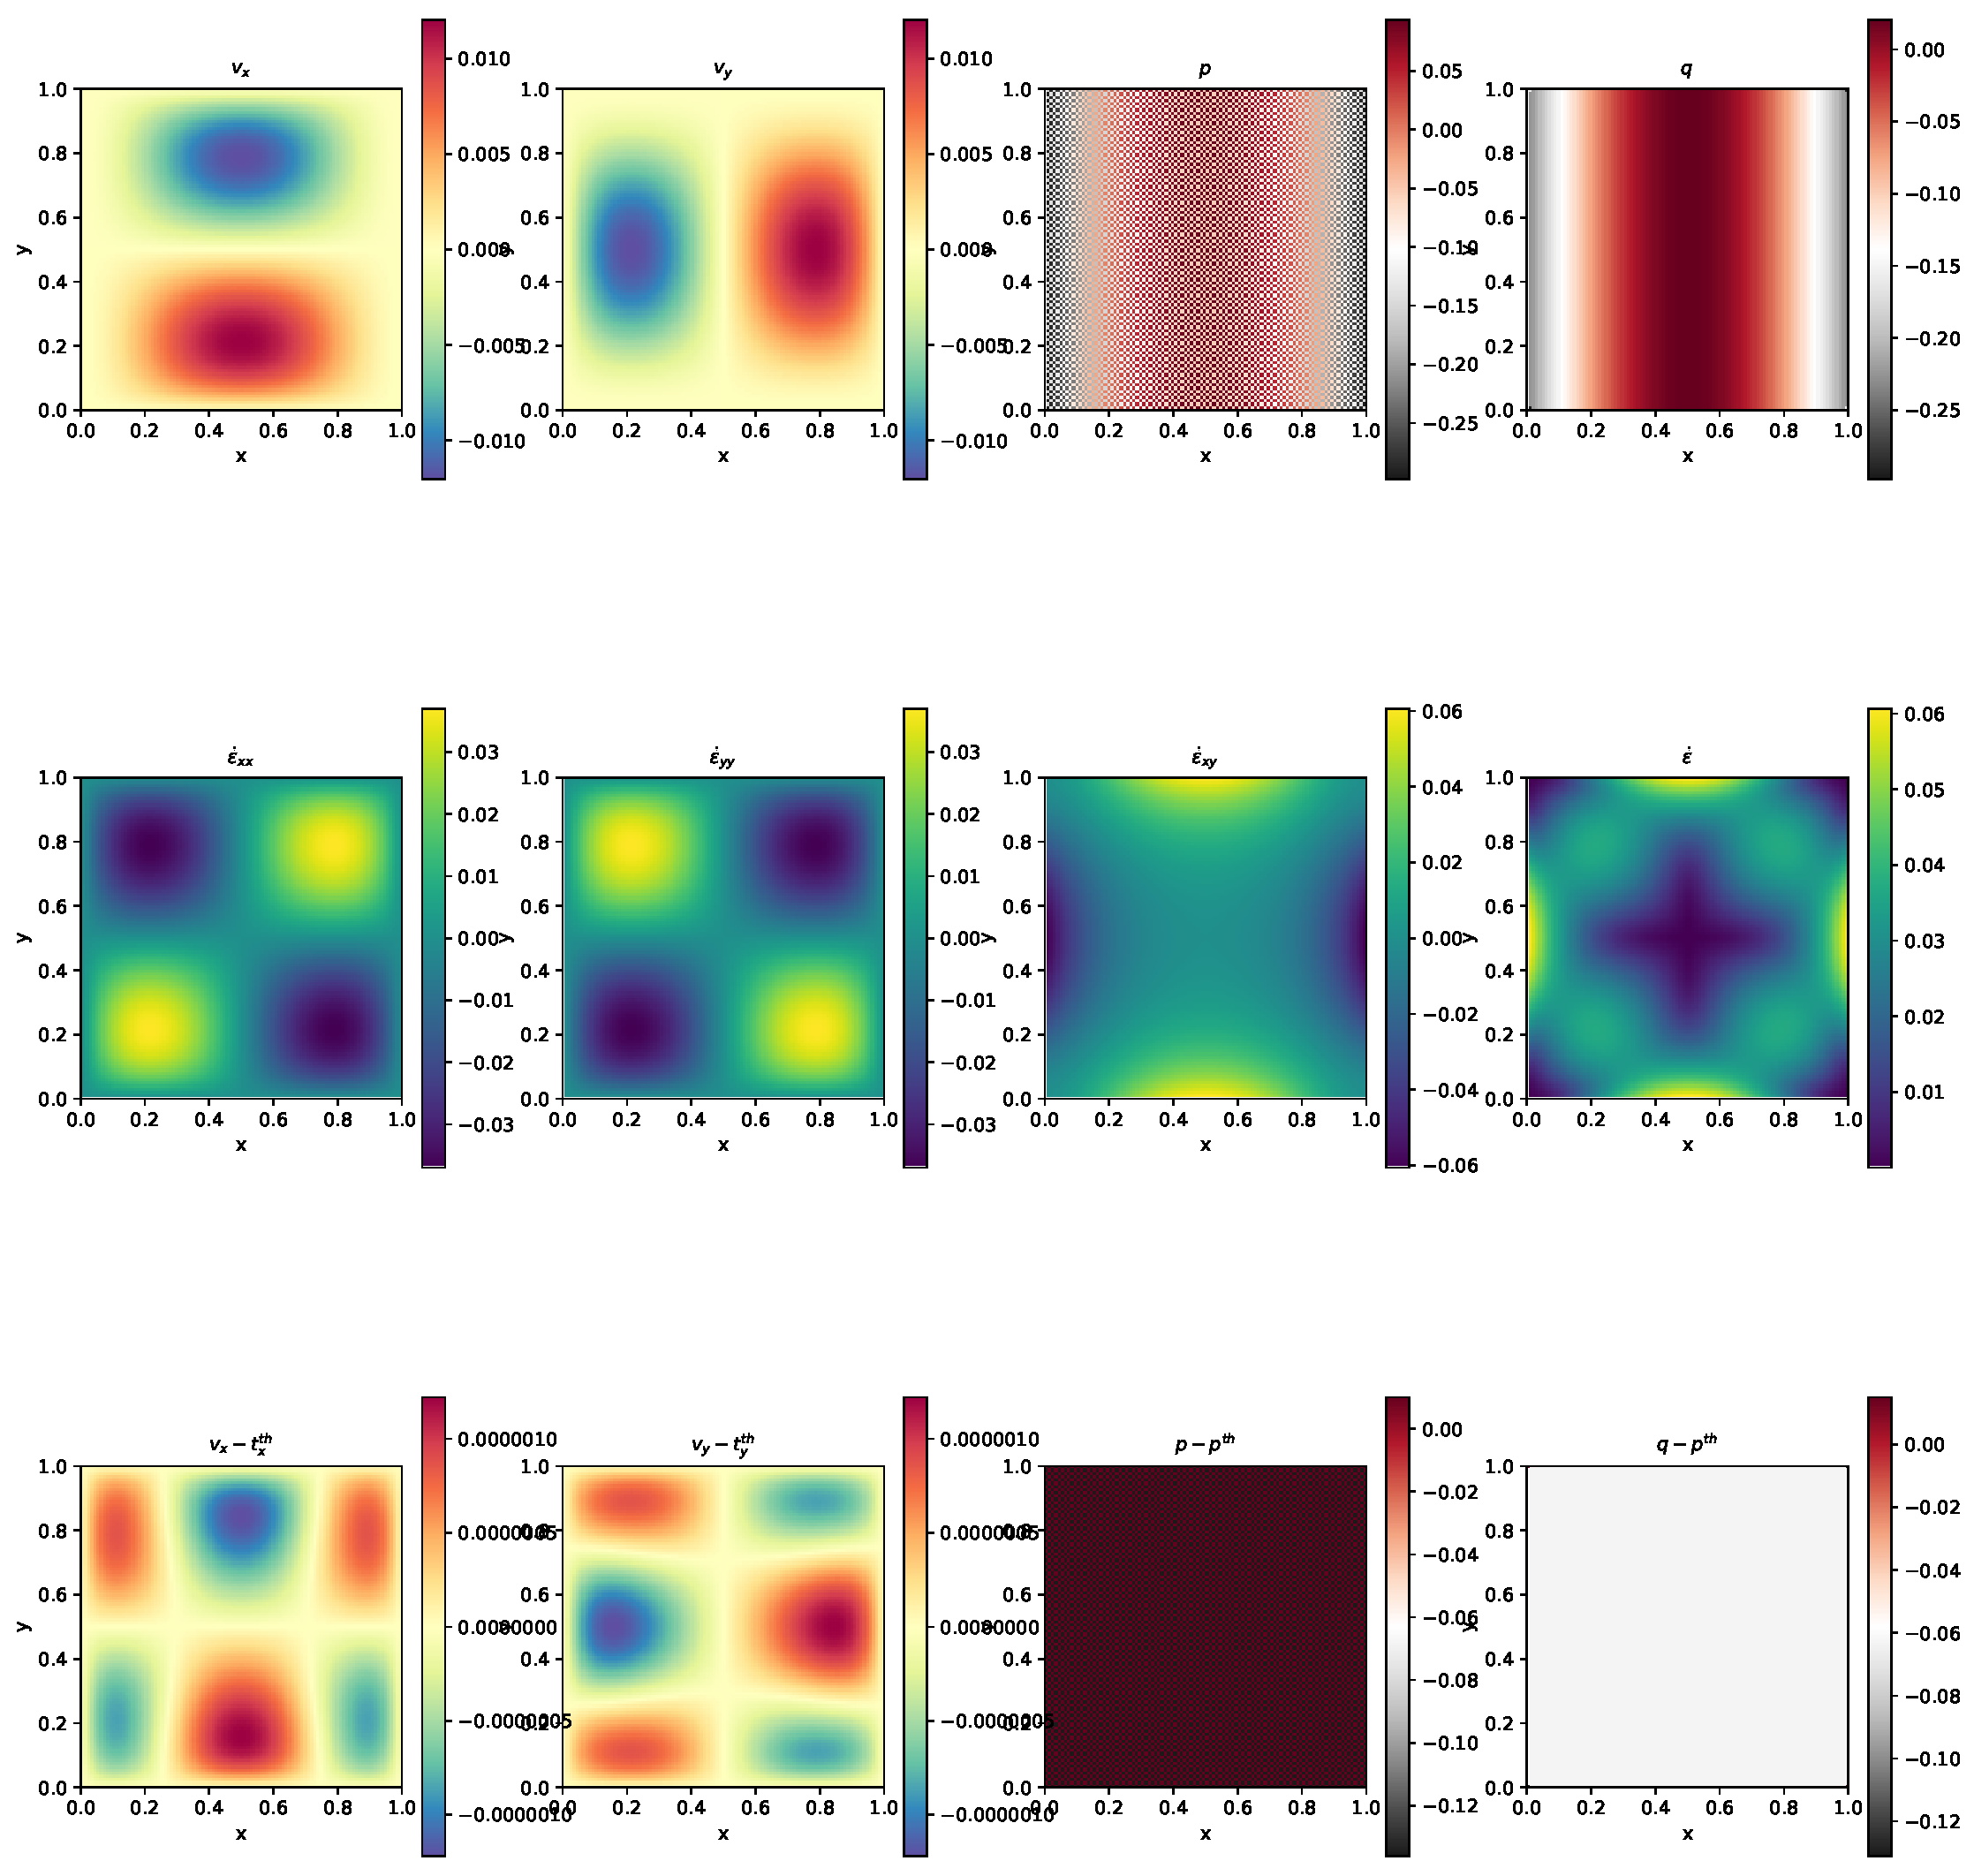
\includegraphics[width=16cm]{python_codes/fieldstone_saddlepoint/solution.pdf}

Unlike the results obtained with the penalty formualtion (see Section \ref{f1}),
the pressure showcases a very strong checkerboard pattern, similar to the one 
in \cite{dohu05}.

\begin{center}
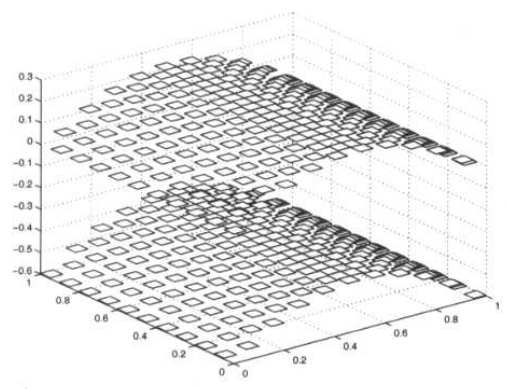
\includegraphics[width=7cm]{python_codes/fieldstone_saddlepoint/doneahuerta}
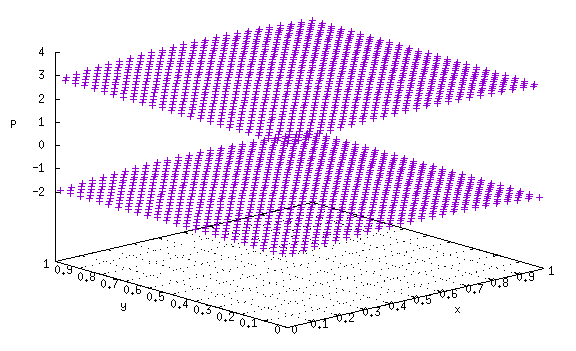
\includegraphics[width=7cm]{python_codes/fieldstone_saddlepoint/mine}\\
Left: pressure solution as shown in \cite{dohu05}; Right: pressure solution obtained
with fieldstone.
\end{center}

Rather interestingly, the nodal pressure (obtained with a simple center-to-node algorithm)
fails to recover a correct pressure at the four corners.


\newpage
%%%%%%%%%%%%%%%%%%%%%%%%%%%%%%%%%%%%%%%%%%%%%%%%%%%%%%%%%%%%%%%%%%%%%%%%%%%%%%%
\section{{\tt fieldstone}: solving the full saddle point problem in 3D}

{\color{red} this does not work because of the Dirichlet b.c. on all 6 sides and all three components}
It does work well with Q2Q1.

This benchmark begins by postulating a polynomial solution to the 3D Stokes equation \cite{dobo04}:
\begin{equation}
{\bm v}
=
\left(
\begin{array}{c}
x+x^2+xy+x^3y \\
y + xy + y^2 + x^2 y^2\\
-2z - 3xz - 3yz - 5x^2 yz
\end{array}
\right)
\label{eqbur}
\end{equation}
and
\begin{equation}
p = xyz + x^3 y^3z - 5/32
\end{equation}
While it is then trivial to verify that this velocity field is divergence-free,  
the corresponding body force of the Stokes equation can be computed by 
inserting this solution into the momentum equation with a given viscosity $\mu$
(constant or position/velocity/strain rate dependent). 
The domain is a unit cube and velocity boundary conditions 
simply use Eq. (\ref{eqbur}). 
Following \cite{busa13}, the viscosity
is given by the smoothly varying function
\begin{equation}
\mu = exp(1 - \beta(x(1 - x) + y(1 - y) + z(1 - z)))
\end{equation}
Choosing $\beta=0$ yields a constant velocity $\mu=e^1$ (and greatly simplifies the right-hand side).
One can easily show that the ratio of viscosities $\mu^\star$
in the system follows $\mu^\star=\exp(-3\beta/4)$ so that choosing $\beta=10$ yields
$\mu^\star\simeq 1808$ and $\beta=20$ yields $\mu^\star\simeq 3.269\times10^6$.


We start from the momentum conservation equation:
\[
-{\bm \nabla}p + {\bm \nabla}\cdot (2 \mu \dot{\bm \epsilon}) = {\bm f}
\]
The $x$-component of this equation writes
\begin{eqnarray}
f_x 
&=& -\frac{\partial p}{\partial x} 
+\frac{\partial}{\partial x} (2\mu \dot{\epsilon}_{xx})
+\frac{\partial}{\partial y} (2\mu \dot{\epsilon}_{xy})
+\frac{\partial}{\partial z} (2\mu \dot{\epsilon}_{xz}) \\
&=& 
-\frac{\partial p}{\partial x} 
+2\mu\frac{\partial}{\partial x} \dot{\epsilon}_{xx}
+2\mu\frac{\partial}{\partial y} \dot{\epsilon}_{xy}
+2\mu\frac{\partial}{\partial z} \dot{\epsilon}_{xz} 
+2\frac{\partial \mu}{\partial x} \dot{\epsilon}_{xx}
+2\frac{\partial \mu}{\partial y} \dot{\epsilon}_{xy}
+2\frac{\partial \mu}{\partial z} \dot{\epsilon}_{xz} 
\end{eqnarray}


Let us compute all the block separately:
\begin{eqnarray}
\dot{\epsilon}_{xx}&=& 1+2x+y+3x^2y  \nonumber\\
\dot{\epsilon}_{yy}&=& 1+x+2y+2x^2y \nonumber\\
\dot{\epsilon}_{zz}&=& -2-3x-3y-5x^2y \nonumber\\
2 \dot{\epsilon}_{xy}&=& (x+x^3)+(y+2xy^2) = x+y+2xy^2+x^3 \nonumber\\
2 \dot{\epsilon}_{xz}&=& (0)+(-3z-10xyz) = -3z -10xyz  \nonumber\\
2 \dot{\epsilon}_{yz}&=& (0) + (-3z-5x^2z) = -3z-5x^2z   \nonumber
\end{eqnarray}
In passing, one can verify that 
$
\dot{\epsilon}_{xx}
+\dot{\epsilon}_{yy}
+\dot{\epsilon}_{zz}=0
$.
We further have
\begin{eqnarray}
\frac{\partial}{\partial x} 2\dot{\epsilon}_{xx}&=& 2(2 +6xy) \nonumber\\ 
\frac{\partial}{\partial y} 2\dot{\epsilon}_{xy}&=&  1+4xy \nonumber\\
\frac{\partial}{\partial z} 2\dot{\epsilon}_{xz}&=& -3 -10xy   \nonumber\\ 
\frac{\partial}{\partial x} 2\dot{\epsilon}_{xy}&=& 1+2y^2+3x^2 \nonumber\\ 
\frac{\partial}{\partial y} 2\dot{\epsilon}_{yy}&=& 2( 2+2x^2 ) \nonumber\\ 
\frac{\partial}{\partial z} 2\dot{\epsilon}_{yz}&=& -3-5x^2   \nonumber\\
\frac{\partial}{\partial x} 2\dot{\epsilon}_{xz}&=& -10yz \nonumber\\ 
\frac{\partial}{\partial y} 2\dot{\epsilon}_{yz}&=& 0  \nonumber\\ 
\frac{\partial}{\partial z} 2\dot{\epsilon}_{zz}&=& 2( 0 ) \nonumber
\end{eqnarray}

\begin{eqnarray}
\frac{\partial p}{\partial x} &=& yz+3x^2y^3z\\
\frac{\partial p}{\partial y} &=& xz +3x^3y^2z \\
\frac{\partial p}{\partial z} &=& xy+x^3y^3
\end{eqnarray}

The viscosity is chosen to be 
\[
\mu(x,y,z) = \exp \left[ 1-\beta ( x(1-x)+y(1-y)+z(1-z) )   \right]
\]

%-----------------------------
\paragraph{Constant viscosity}

Setting $\beta=0$ yields 
\[
\mu(x,y,z) = e \simeq 2.718
\]
so that 
\begin{eqnarray}
\frac{\partial }{\partial x} \mu(x,y,z) &=& 0 \\
\frac{\partial }{\partial y} \mu(x,y,z) &=& 0 \\
\frac{\partial }{\partial z} \mu(x,y,z) &=& 0
\end{eqnarray}
and 
\begin{eqnarray}
f_x 
&=& 
-\frac{\partial p}{\partial x} 
+2\mu\frac{\partial}{\partial x} \dot{\epsilon}_{xx}
+2\mu\frac{\partial}{\partial y} \dot{\epsilon}_{xy}
+2\mu\frac{\partial}{\partial z} \dot{\epsilon}_{xz} \nonumber\\
&=&
-(yz+3x^2y^3z)
+ 2(2 +6xy) + (1+4xy) + (-3 -10xy)   \\
&=&
-(yz+3x^2y^3z)
+\mu(2+6xy ) \\
f_y 
&=&  
-\frac{\partial p}{\partial y} 
+2\mu\frac{\partial}{\partial x} \dot{\epsilon}_{xy}
+2\mu\frac{\partial}{\partial y} \dot{\epsilon}_{yy}
+2\mu\frac{\partial}{\partial z} \dot{\epsilon}_{yz}  \nonumber\\
&=&
-(xz +3x^3y^2z)
+
\mu(1+2y^2+3x^2)
+\mu2( 2+2x^2 )  
+\mu(-3-5x^2) \\
&=&
-(xz +3x^3y^2z)
+ \mu ( 2 + 2x^2 +  2y^2)
\\ 
f_z 
&=&
-\frac{\partial p}{\partial z} 
+2\mu\frac{\partial}{\partial x} \dot{\epsilon}_{xz}
+2\mu\frac{\partial}{\partial y} \dot{\epsilon}_{yz}
+2\mu\frac{\partial}{\partial z} \dot{\epsilon}_{zz}  \nonumber\\
&=&
-(xy+x^3y^3) 
+ \mu (-10yz) + 0 + 0 \\
&=&
-(xy+x^3y^3) 
+\mu (-10yz) 
\end{eqnarray}

finally

\[
{\bm f} = 
-
\left(
\begin{array}{c}
yz+3x^2y^3z\\
xz +3x^3y^2z \\
xy+x^3y^3
\end{array}
\right)
+\mu
\left(
\begin{array}{c}
2+6xy  \\
2 + 2x^2 +  2y^2 \\
-10yz 
\end{array}
\right)
\]

$\Rightarrow$ sign problem with Burstedde et al Eq 26 !!



%-----------------------------
\paragraph{Variable viscosity}

\begin{eqnarray}
\frac{\partial }{\partial x} \mu(x,y,z) &=& -(1-2x)\beta \mu(x,y,z) \nonumber\\
\frac{\partial }{\partial y} \mu(x,y,z) &=& -(1-2y)\beta \mu(x,y,z) \nonumber\\
\frac{\partial }{\partial z} \mu(x,y,z) &=& -(1-2z)\beta \mu(x,y,z) \nonumber
\end{eqnarray}

\begin{eqnarray}
{\bm f} 
&=& 
-
\left(
\begin{array}{c}
yz+3x^2y^3z\\
xz +3x^3y^2z \\
xy+x^3y^3
\end{array}
\right)
+\mu
\left(
\begin{array}{c}
2+6xy  \\
2 + 2x^2 +  2y^2 \\
-10yz 
\end{array}
\right) \\
&&
-(1-2x)\beta \mu (x,y,z)
\left(
\begin{array}{c}
2\dot{\epsilon}_{xx} \\
2\dot{\epsilon}_{xy} \\
2\dot{\epsilon}_{xz} \\
\end{array}
\right)
-(1-2y)\beta \mu (x,y,z)
\left(
\begin{array}{c}
2\dot{\epsilon}_{xy} \\
2\dot{\epsilon}_{yy} \\
2\dot{\epsilon}_{yz} \\
\end{array}
\right)
-(1-2z)\beta \mu (x,y,z)
\left(
\begin{array}{c}
2\dot{\epsilon}_{xz} \\
2\dot{\epsilon}_{yz} \\
2\dot{\epsilon}_{zz} \\
\end{array}
\right) \nonumber\\
&=& 
-
\left(
\begin{array}{c}
yz+3x^2y^3z\\
xz +3x^3y^2z \\
xy+x^3y^3
\end{array}
\right)
+\mu
\left(
\begin{array}{c}
2+6xy  \\
2 + 2x^2 +  2y^2 \\
-10yz 
\end{array}
\right) \nonumber\\
&-&
(1-2x)\beta \mu 
\left(
\begin{array}{c}
2+4x+2y+6x^2y \\
x+y+2xy^2+x^3 \\
-3z -10xyz 
\end{array}
\right)
-(1-2y)\beta \mu 
\left(
\begin{array}{c}
x+y+2xy^2+x^3 \\
2+2x+4y+4x^2y \\
-3z-5x^2z \\
\end{array}
\right)
-(1-2z)\beta \mu
\left(
\begin{array}{c}
-3z -10xyz \\
-3z-5x^2z \\
-4-6x-6y-10x^2y
\end{array}
\right) \nonumber
\end{eqnarray}

at $(x,y,z)=(0,0,0)$, $\mu=\exp(1)$, 

at $(x,y,z)=(0.5,0.5,0.5)$, $\mu=\exp(1-3\beta/4)$

Viscosity ratio is given by 
\[
\mu^\star = \frac{\exp(1-3\beta/4)}{\exp(1)} = \exp(-3\beta/4)
\]
By varying $\beta$ between 1 and 22 we can get up to 7 orders of magnitude viscosity difference !

























\fbox{
\parbox{10cm}{{\bf features}
\begin{itemize}
\item $Q_1\times P_0$ element
\item incompressible flow
\item saddle point system
\item Dirichlet boundary conditions (free-slip)
\item direct solver
\item isothermal
\item non-isoviscous
\item 3D
\item elemental b.c. 
\item analytical solution
\end{itemize}
}}


%\begin{center}
%\includegraphics[width=5cm]{python_codes/fieldstone_stokes_sphere_3D/grid}
%\includegraphics[width=5cm]{python_codes/fieldstone_stokes_sphere_3D/vel}
%\includegraphics[width=5cm]{python_codes/fieldstone_stokes_sphere_3D/press}\\
%\includegraphics[width=5cm]{python_codes/fieldstone_stokes_sphere_3D/press2}
%\includegraphics[width=5cm]{python_codes/fieldstone_stokes_sphere_3D/visc}
%\includegraphics[width=5cm]{python_codes/fieldstone_stokes_sphere_3D/dens}\\
%{\small resolution is 24x24x24}
%\end{center}



\newpage
%%%%%%%%%%%%%%%%%%%%%%%%%%%%%%%%%%%%%%%%%%%%%%%%%%%%%%%%%%%%%%%%%%%%%%%%%%%%%%%
\section{{\tt fieldstone}: solving the full saddle point problem with $Q_2\times Q_1$ elements}
The details of the numerical setup are presented in Section \ref{f1}.

Each element has $m_V=9$ vertices so in total $ndof_V\times m_V=18$ velocity dofs and 
$ndof_P*m_P=4$ pressure dofs. The total number of 
velocity dofs is therefore $NfemV=nnp \times ndofV$ while the total number of
pressure dofs is $NfemP=nel$. The total number of dofs is then $Nfem=NfemV+NfemP$.

As a consequence, matrix $\K$ has size $NfemV,NfemV$ and matrix $\G$ has size $NfemV,NfemP$.
Vector $f$ is of size $NfemV$ and vector $h$ is of size $NfemP$.  

\begin{center}
\includegraphics[width=12cm]{python_codes/fieldstone_saddlepoint_q2q1/q2q1setup}\\
{\color{red} renumber all nodes to start at zero!! Also internal numbering does not work here }
\end{center}


ToDo:
\begin{itemize}
\item normalise pressure 
\end{itemize}

\fbox{
\parbox{10cm}{{\bf features}
\begin{itemize}
\item $Q_2\times Q_1$ element \index{$Q_2 \times Q_1$}
\item incompressible flow \index{incompressible flow}
\item mixed formulation \index{mixed formulation}
\item Dirichlet boundary conditions (no-slip)
\item isothermal \index{isothermal}
\item isoviscous \index{isoviscous}
\item analytical solution \index{analytical solution}
\end{itemize}
}}

\begin{center}
\includegraphics[width=10cm]{python_codes/fieldstone_saddlepoint_q2q1/errors}
\end{center}


\newpage
%%%%%%%%%%%%%%%%%%%%%%%%%%%%%%%%%%%%%%%%%%%%%%%%%%%%%%%%%%%%%%%%%%%%%%%%%%%%%%%
\section{{\tt fieldstone}: solving the full saddle point problem with $Q_3\times Q_2$ elements}
The details of the numerical setup are presented in Section \ref{f1}.

Each element has $m_V=16$ vertices so in total $ndof_V\times m_V=32$ 
velocity dofs and 
$ndof_P*m_P=9$ pressure dofs. The total number of 
velocity dofs is therefore $NfemV=nnp \times ndofV$ while the total number of
pressure dofs is $NfemP=nel$. The total number of dofs is then $Nfem=NfemV+NfemP$.

As a consequence, matrix $\K$ has size $NfemV,NfemV$ and matrix $\G$ has size $NfemV,NfemP$.
Vector $f$ is of size $NfemV$ and vector $h$ is of size $NfemP$.  

\begin{verbatim}

60===61===62===63===64===65===66===67===68===70
||             ||             ||             ||
50   51   52   53   54   55   56   57   58   59
||             ||             ||             ||
40   41   42   43   44   45   46   47   48   49
||             ||             ||             ||
30===31===32===33===34===35===36===37===38===39
||             ||             ||             ||
20   21   22   23   24   25   26   27   28   29
||             ||             ||             ||
10   11   12   13   14   15   16   17   18   19
||             ||             ||             ||
00===01===02===03===04===05===06===07===08===09

Example of 3x2 mesh. nnx=10, nny=7, nnp=70, nelx=3, nely=2, nel=6
\end{verbatim}


\begin{verbatim}
12===13===14===15           06=====07=====08
||   ||   ||   ||           ||     ||     ||
08===09===10===11           ||     ||     ||
||   ||   ||   ||           03=====04=====05
04===05===06===07           ||     ||     ||
||   ||   ||   ||           ||     ||     ||
00===01===02===03           00=====01=====02

Velocity (Q3)               Pressure (Q2)

(r,s)_{00}=(-1,-1)          (r,s)_{00}=(-1,-1) 
(r,s)_{01}=(-1/3,-1)        (r,s)_{01}=(0,-1) 
(r,s)_{02}=(+1/3,-1)        (r,s)_{02}=(+1,-1) 
(r,s)_{03}=(+1,-1)          (r,s)_{03}=(-1,0) 
(r,s)_{04}=(-1,-1/3)        (r,s)_{04}=(0,0) 
(r,s)_{05}=(-1/3,-1/3)      (r,s)_{05}=(+1,0) 
(r,s)_{06}=(+1/3,-1/3)      (r,s)_{06}=(-1,+1) 
(r,s)_{07}=(+1,-1/3)        (r,s)_{07}=(0,+1) 
(r,s)_{08}=(-1,+1/3)        (r,s)_{08}=(+1,+1) 
(r,s)_{09}=(-1/3,+1/3)
(r,s)_{10}=(+1/3,+1/3)
(r,s)_{11}=(+1,+1/3)
(r,s)_{12}=(-1,+1)
(r,s)_{13}=(-1/3,+1)
(r,s)_{14}=(+1/3,+1)
(r,s)_{15}=(+1,+1)

\end{verbatim}



The velocity shape functions are given by:
\begin{eqnarray}
N_1(r)&=&(-1   +r +9r^2 - 9r^3)/16 \nonumber\\
N_2(r)&=&(+9 -27r -9r^2 +27r^3)/16 \nonumber\\
N_3(r)&=&(+9 +27r -9r^2 -27r^3)/16 \nonumber\\
N_4(r)&=&(-1   -r +9r^2 + 9r^3)/16 \nonumber
\end{eqnarray}

\begin{eqnarray}
N_1(t)&=&(-1   +t +9t^2 - 9t^3)/16 \nonumber\\
N_2(t)&=&(+9 -27t -9t^2 +27t^3)/16 \nonumber\\
N_3(t)&=&(+9 +27t -9t^2 -27t^3)/16 \nonumber\\
N_4(t)&=&(-1   -t +9t^2 + 9t^3)/16 \nonumber
\end{eqnarray}

\begin{eqnarray}
N_01(r,t)&=&N_1(r)N_1(t) \\
N_02(r,t)&=&N_2(r)N_1(t) \\
N_03(r,t)&=&N_3(r)N_1(t) \\
N_04(r,t)&=&N_4(r)N_1(t) \\
N_05(r,t)&=&N_1(r)N_2(t) \\
N_06(r,t)&=&N_2(r)N_2(t) \\
N_07(r,t)&=&N_3(r)N_2(t) \\
N_08(r,t)&=&N_4(r)N_2(t) \\
N_09(r,t)&=&N_1(r)N_3(t) \\
N_10(r,t)&=&N_2(r)N_3(t) \\
N_11(r,t)&=&N_3(r)N_3(t) \\
N_12(r,t)&=&N_4(r)N_3(t) \\
N_13(r,t)&=&N_1(r)N_4(t) \\
N_14(r,t)&=&N_2(r)N_4(t) \\
N_15(r,t)&=&N_3(r)N_4(t) \\
N_16(r,t)&=&N_4(r)N_4(t) 
\end{eqnarray}

and their derivatives:






{\color{red} Write about 4 point quadrature}.








\fbox{
\parbox{10cm}{{\bf features}
\begin{itemize}
\item $Q_3\times Q_2$ element \index{$Q_3 \times Q_2$}
\item incompressible flow \index{incompressible flow}
\item mixed formulation \index{mixed formulation}
\item isothermal \index{isothermal}
\item isoviscous \index{isoviscous}
\item analytical solution \index{analytical solution}
\end{itemize}
}}

\begin{center}
\includegraphics[width=10cm]{python_codes/fieldstone_saddlepoint_q3q2/errors}
\end{center}

velocity error rate is cubic, pressure superconvergent since the pressure field
is quadratic and therefore lies into the Q2 space.


\newpage
%%%%%%%%%%%%%%%%%%%%%%%%%%%%%%%%%%%%%%%%%%%%%%%%%%%%%%%%%%%%%%%%%%%%%%%%%%%%%%%
\section{{\tt fieldstone}: the Busse benchmark}

This three-dimensional benchmark was first proposed by \cite{bucc93}. 
It has been subsequently presented in \cite{tack94,trha98,albe00,omma06,dawk11,krhb12}.
We here focus on Case 1 of \cite{bucc93}:  an isoviscous bimodal convection experiment at $Ra=3\times 10^5$.

The domain is of size $a\times b\times h$ with $a=1.0079h$, $b=0.6283h$ with $h=2700$km. It is filled with a Newtonian fluid
characterised by $\rho_0=3300{\rm kg}.{\rm m}^{-3}$, $\alpha=10^{-5}{\rm K}^{-1}$, $\mu=8.0198\times10^{23}{\rm Pa.s}$, 
$k=3.564{\rm W}.{\rm m}^{-1}.{\rm K}^{-1}$, 
$c_p=1080{\rm J}.{\rm K}^{-1}.{\rm kg}^{-1}$.
The gravity vector is set to ${\bm g}=(0,0,-10)^T$.
The temperature is imposed at the bottom  ($T=3700^\circ$C) and at the top ($T=0^\circ$C).

The various measurements presented in \cite{bucc93} are listed hereafter:
\begin{itemize}
\item The Nusselt number $Nu$ computed at the top surface following Eq. (\ref{eqNu}):
\[
Nu = L_z \frac{\int\int_{z=L_z} \frac{\partial T}{\partial y} dx dy  }{\int \int_{z=0} T dx dy}
\]
\item the root mean square velocity $v_{rms}$ and the temperature mean square velocity $T_{rms}$
\item The vertical velocity $w$ and temperature $T$ at points ${\bm x}_1=(0,0,L_z/2)$, ${\bm x}_2=(L_x,0,L_z/2)$,
${\bm x}_3=(0,L_y,L_z/2)$ and ${\bm x}_4=(L_x,L_y,L_z/2)$;
\item the vertical component of the heat flux $Q$ at the top surface  at all four corners.
\end{itemize}

The values plotted hereunder are adimensionalised by means of a reference temperature (3700K),
a reference lengthscale 2700km, and a reference time $L_z^2/\kappa$. 




\fbox{
\parbox{10cm}{{\bf features}
\begin{itemize}
\item $Q_1\times P_0$ element
\item incompressible flow
\item mixed formulation
\item Dirichlet boundary conditions (free-slip)
\item direct solver
\item isothermal
\item non-isoviscous
\item 3D
\item elemental b.c. 
\item buoyancy driven
\end{itemize}
}}




\newpage
%%%%%%%%%%%%%%%%%%%%%%%%%%%%%%%%%%%%%%%%%%%%%%%%%%%%%%%%%%%%%%%%%%%%%%%%%%%%%%%
\section{{\tt fieldstone}: The non-conforming $Q_1 \times P_0$ element} \label{ncq1p0} 


\fbox{
\parbox{10cm}{{\bf features}
\begin{itemize}
\item Non-conforming $Q_1\times P_0$ element \index{nonconforming $Q_1 \times P_0$}
\item incompressible flow \index{incompressible flow}
\item mixed formulation \index{mixed formulation}
\item isothermal \index{isothermal}
\item non-isoviscous \index{non-isoviscous}
\item analytical solution \index{analytical solution}
\item pressure smoothing \index{pressure smoothing} 
\end{itemize}
}}

try Q1 mapping instead of isoparametric.

%\includegraphics[width=16cm]{python_codes/fieldstone_saddlepoint/solution.pdf}



\newpage
%%%%%%%%%%%%%%%%%%%%%%%%%%%%%%%%%%%%%%%%%%%%%%%%%%%%%%%%%%%%%%%%%%%%%%%%%%%%%%%
\section{{\tt fieldstone}: The stabilised $Q_1 \times Q_1$ element} 
The details of the numerical setup are presented in Section \ref{f1}.



\newpage
%%%%%%%%%%%%%%%%%%%%%%%%%%%%%%%%%%%%%%%%%%%%%%%%%%%%%%%%%%%%%%%%%%%%%%%%%%%%%%%
\section{{\tt fieldstone}: compressible flow (1)}
We first start with an isothermal Stokes flow, so that we disregard the heat transport equation and 
the equations we wish to solve are simply:

\begin{align}
  \label{eq:stokes-1}
  -\nabla \cdot \left[2\eta \left(\dot\varepsilon(\bm v)
                                  - \frac{1}{3}(\nabla \cdot \bm v)\mathbf 1\right)
                \right] + \nabla p &=
  \rho \bm g
  &
  & \textrm{in $\Omega$},
  \\
  \label{eq:stokes-2}
  \nabla \cdot (\rho \bm v) &= 0
  &
  & \textrm{in $\Omega$}
\end{align}
The second equation can be rewritten 
$\nabla \cdot (\rho {\bm v}) =  \rho \nabla \cdot {\bm v} + {\bm v} \cdot {\bm \nabla}\rho=0$
or, 
\[
\nabla \cdot {\bm v} + \frac{1}{\rho} {\bm v} \cdot {\bm \nabla}\rho=0
\]
Note that this presupposes that the density is not zero anywhere in the domain.

We use a mixed formulation and therefore  
keep both velocity and pressure as unknowns. We end up having to solve 
the following system:
\[
\left(
\begin{array}{cc}
\K & \G \\ \G^T+\Z & 0 
\end{array}
\right)
\cdot
\left(
\begin{array}{c}
{\cal V} \\ {\cal P}
\end{array}
\right)
=
\left(
\begin{array}{c}
 f \\ h
\end{array}
\right)
\quad\quad
{\rm or,}
\quad\quad
\A \cdot X = rhs
\]
Where $\K$ is the stiffness matrix, $\G$ is the discrete gradient operator, 
$\G^T$ is the discrete divergence operator, ${\cal V}$ the velocity vector, 
${\cal P}$ the pressure vector.
Note that the term $\Z{\cal V}$ derives from term ${\bm v} \cdot {\bm \nabla} \rho$ in the continuity equation. 

Each block $\K$, $\G$ , $\Z$ and vectors $f$ and $h$ are built separately 
in the code and assembled into 
the matrix $\A$ and vector $rhs$ afterwards. $\A$ and $rhs$ are then passed to the solver. 
We will see later that there are alternatives to solve this approach which do not require to 
build the full Stokes matrix $\A$. 

{\sl Remark}: the term $\Z {\cal V}$ is often put in the rhs (i.e. added to $h$) so that 
the matrix $\A$ retains the same structure as in the incompressible case. This is indeed 
how it is implemented in ASPECT. 

In the case of a compressible flow the strain rate tensor and the deviatoric strain rate tensor are no more equal (since ${\bm \nabla}\cdot{\bm v} \neq 0$).
The deviatoric strainrate tensor is given by\footnote{See the ASPECT manual for a justification of the 3 value in the denominator in 2D and 3D.} 
\[
\dot{\bm \epsilon}^d({\bm v})=
\dot{\bm \epsilon}({\bm v})-\frac{1}{3} Tr(\dot{\bm \epsilon}) {\bm 1}
=\dot{\bm \epsilon}({\bm v})-\frac{1}{3} ({\bm \nabla}\cdot{\bm v}) {\bm 1}
\]
In that case:
\begin{eqnarray}
\dot{\epsilon}_{xx}^d 
&=& \frac{\partial u}{\partial x}
-\frac{1}{3} \left( \frac{\partial u}{\partial x} + \frac{\partial v}{\partial y} \right) 
= \frac{2}{3}\frac{\partial u}{\partial x}
-\frac{1}{3} \frac{\partial v}{\partial y}
%=
%\frac{2}{3} \sum_{i=1}^4 \frac{\partial N_i}{\partial x}\;  u_i 
%-\frac{1}{3} \sum_{i=1}^4 \frac{\partial N_i}{\partial y}\;  v_i 
\\
\dot{\epsilon}_{yy}^d 
&=& \frac{\partial v}{\partial y}
-\frac{1}{3} \left( \frac{\partial u}{\partial x} + \frac{\partial v}{\partial y} \right) 
=-\frac{1}{3} \frac{\partial u}{\partial x} 
+ \frac{2}{3} \frac{\partial v}{\partial y} 
%=-\frac{1}{3}  \sum_{i=1}^4 \frac{\partial N_i}{\partial x}\;  u_i
%+ \frac{2}{3} \sum_{i=1}^4 \frac{\partial N_i}{\partial y}\;  v_i
\\
2\dot{\epsilon}_{xy}^d 
&=& 
\frac{\partial u}{\partial y} 
+\frac{\partial v}{\partial x} 
%= \sum_{i=1}^4 \frac{\partial N_i}{\partial y}\;  u_i
%+ \sum_{i=1}^4 \frac{\partial N_i}{\partial x}\;  v_i
\end{eqnarray}
and then 
\[
\dot{\bm \epsilon}^d({\bm v})
=
\left(
\begin{array}{cc}
\frac{2}{3} \frac{\partial u}{\partial x} -\frac{1}{3} \frac{\partial v}{\partial y} &
\frac{1}{2}\frac{\partial u}{\partial y} + \frac{1}{2}\frac{\partial v}{\partial x}  \\ \\
\frac{1}{2}\frac{\partial u}{\partial y} + \frac{1}{2}\frac{\partial v}{\partial x}  &
-\frac{1}{3} \frac{\partial u}{\partial x} +\frac{2}{3} \frac{\partial v}{\partial y} 
\end{array}
\right)
\]

From $\vec{\tau} = 2\eta \vec{\epsilon}^d$ we arrive at:
\[
\left(
\begin{array}{c}
\tau_{xx}\\
\tau_{yy}\\
\tau_{xy}\\
\end{array}
\right)
=
2\eta
\left(
\begin{array}{c}
\dot{\epsilon}_{xx}^d \\
\dot{\epsilon}_{yy}^d \\
\dot{\epsilon}_{xy}^d 
\end{array}
\right)
=2 \eta
\left(
\begin{array}{ccc}
2/3 & -1/3& 0 \\
-1/3 & 2/3 & 0 \\
0 & 0 & 1/2 \\
\end{array}
\right)
\cdot 
\left(
\begin{array}{c}
\frac{\partial u}{\partial x} \\ 
\frac{\partial v}{\partial y} \\ 
\frac{\partial u}{\partial y}\! +\! \frac{\partial v}{\partial x} \\
\end{array}
\right)
=
\eta
\left(
\begin{array}{ccc}
4/3 & -2/3& 0 \\
-2/3 & 4/3 & 0 \\
0 & 0 & 1 \\
\end{array}
\right)
\cdot 
\left(
\begin{array}{c}
\frac{\partial u}{\partial x} \\ 
\frac{\partial v}{\partial y} \\ 
\frac{\partial u}{\partial y}\! +\! \frac{\partial v}{\partial x} \\
\end{array}
\right)
\]
or, 
\[
\vec{\tau} = {\bm C}_\eta {\bm B} V
\]


















\newpage
In order to test our implementation we have created a few manufactured solutions:
\begin{itemize}
\item benchmark \#1 ({\tt ibench=1})): Starting from a density profile of:
\begin{equation}
    \rho = xy
\end{equation}
We derive a velocity given by:
\begin{equation}
    v_x = \frac{C_x}{x} , v_y = \frac{C_y}{y}
\end{equation}

With $g_x = \frac{1}{x}$ and $g_y = \frac{1}{y}$, this leads us to a pressure profile:
\begin{equation}
    p = - \mu \left( \frac{C_x}{x^2} + \frac{C_y}{y^2} \right)  + xy + C_0
\end{equation}
This gives us a strain rate:
\begin{align}
    \begin{split}
        e_{xx} =  \frac{-C_x}{x^2}
        \\
        e_{yy} =  \frac{-C_y}{y^2}
    \end{split}
\end{align}

 
\item benchmark \#2 ({\tt ibench=2}): Starting from a density profile of:
\begin{equation}
    \rho = cos(x)cos(y)
\end{equation}
We derive a velocity given by:
\begin{equation}
    v_x = \frac{C_x}{cos(x)} , v_y = \frac{C_y}{cos(y)}
\end{equation}
With $g_x = \frac{1}{cos(x)}$ and $g_y = \frac{1}{cos(y)}$, this leads us to a pressure profile:
\begin{equation}
    p =  \mu \Bigg(\frac{C_x sin(x)}{cos^2(x)} + \frac{C_y sin(y)}{cos^2(y)}\Bigg) 
    -( sin(x) + sin(y) ) + C_0
\end{equation}
\begin{align}
    \begin{split}
        e_{xx} = C_x \frac{sin(x)}{cos^2(x)}
        \\
        e_{yy} = C_y \frac{sin(y)}{cos^2(y)}
    \end{split}
\end{align}



\item benchmark \#3 
\item benchmark \#4 
\item benchmark \#5 
\end{itemize}




\fbox{
\parbox{10cm}{{\bf features}
\begin{itemize}
\item $Q_1\times P_0$ element \index{$Q_1 \times P_0$}
\item incompressible flow \index{incompressible flow}
\item mixed formulation \index{mixed formulation}
\item Dirichlet boundary conditions (no-slip)
\item direct solver (?)
\item isothermal \index{isothermal}
\item isoviscous \index{isoviscous}
\item analytical solution \index{analytical solution}
\item pressure smoothing \index{pressure smoothing} 
\end{itemize}
}}

%\includegraphics[width=16cm]{python_codes/fieldstone_saddlepoint/solution.pdf}




\newpage
%%%%%%%%%%%%%%%%%%%%%%%%%%%%%%%%%%%%%%%%%%%%%%%%%%%%%%%%%%%%%%%%%%%%%%%%%%%%%%%
\section{{\tt fieldstone}: compressible flow (2)}
Let us start with some thermodynamics. Every material has an equation of state.
The equilibrium thermodynamic state of any material can
be constrained if any two state variables are specified.
Examples of state variables include
the pressure $p$ and specific volume $\nu = 1/\rho$, as well as the temperature $T$.

After linearisation, the density depends on temperature and pressure as follows:
\[
\rho(T,p) = \rho_0 \left((1 - \alpha(T-T_0) + \beta_T p \right)
\]
where $\alpha$ is the coefficient of thermal expansion, also called 
thermal expansivity: \index{thermal expansion}
\[
\alpha=-\frac{1}{\rho}\left( \frac{\partial \rho}{\partial T} \right)_p
\]
$\alpha$ is the percentage increase in volume of a material per degree of temperature increase; the
subscript $p$ means that the pressure is held fixed.

$\beta_T$ is the isothermal compressibility of the fluid, which is given by \index{compressibility}
\[
\beta_T = \frac{1}{K} = \frac{1}{\rho}\left( \frac{\partial \rho}{\partial P} \right)_T
\]
with $K$ the bulk modulus. \index{bulk modulus}
%aspect manual
Values of $\beta_T=10^{-12}-10^{-11}$ Pa$^{-1}$ are reasonable for Earth's mantle, with values decreasing by about a
factor of 5 between the shallow lithosphere and core-mantle boundary.
This is the percentage increase in density per unit change in pressure at constant temperature.
Both the coefficient of thermal expansion and the isothermal compressibility can be obtained
from the equation of state.

The full set of equations we wish to solve is given by

\begin{eqnarray}
-\nabla \cdot \left[2\eta \dot{\bm \epsilon}^d({\bm v}) \right] + \nabla p &=& \rho_0 \left((1 - \alpha(T-T_0) + \beta_T p \right) {\bm g} \quad\quad \textrm{in $\Omega$}  \label{eq:stokes-1} \\
\nabla \cdot {\bm v} + \frac{1}{\rho} {\bm v} \cdot {\bm \nabla}\rho&=&0 \quad\quad  \textrm{in $\Omega$}   \label{eq:stokes-2} \\
\rho C_p \left(\frac{\partial T}{\partial t} + \bm v\cdot\nabla T\right) - \nabla\cdot k\nabla T   &=& 
  \rho H  +  2\eta \dot{\bm \epsilon}^d : \dot{\bm \epsilon}^d    +\alpha T \left( \frac{\partial p}{\partial t}+  \bm v \cdot \nabla p \right) 
\quad\quad   \textrm{in $\Omega$},
  \label{eq:temperature}
\end{eqnarray}

Note that this presupposes that the density is not zero anywhere in the domain.

We use a mixed formulation and therefore  
keep both velocity and pressure as unknowns. We end up having to solve 
the following system:
\[
\left(
\begin{array}{cc}
\K & \G+\W \\ \G^T+\Z & 0 
\end{array}
\right)
\cdot
\left(
\begin{array}{c}
{\cal V} \\ {\cal P}
\end{array}
\right)
=
\left(
\begin{array}{c}
 f \\ h
\end{array}
\right)
\quad\quad
{\rm or,}
\quad\quad
\A \cdot X = rhs
\]
Where $\K$ is the stiffness matrix, $\G$ is the discrete gradient operator, 
$\G^T$ is the discrete divergence operator, ${\cal V}$ the velocity vector, 
${\cal P}$ the pressure vector.
Note that the term $\Z{\cal V}$ derives from term ${\bm v} \cdot {\bm \nabla} \rho$ in the continuity equation. 

As perfectly explained in the step 32 of deal.ii\footnote{https://www.dealii.org/9.0.0/doxygen/deal.II/step\_32.html},
we need to scale the $\G$ term since it is many orders of magnitude smaller than $\K$, which introduces large inaccuracies in the solving process to the point that the solution is nonsensical. This scaling coefficient is $\eta/L$. After building the $\G$ block, it is then scaled as follows: $\G'=\frac{\eta}{L}\G$ so that we now solve 

\[
\left(
\begin{array}{cc}
\K & \G'+\W \\ \G'^T+\Z & 0 
\end{array}
\right)
\cdot
\left(
\begin{array}{c}
{\cal V} \\ {\cal P}'
\end{array}
\right)
=
\left(
\begin{array}{c}
 f \\ h
\end{array}
\right)
\]
After the solve phase, we recover the real pressure with ${\cal P}=\frac{\eta}{L}{\cal P}'$.

{\color{red} adapt notes since I should scale $\W$ and $\Z$ too}.
{\color{red} $h$ should be caled too !!!!!!!!!!!!!!!} 

Each block $\K$, $\G$ , $\Z$ and vectors $f$ and $h$ are built separately 
in the code and assembled into 
the matrix $\A$ and vector $rhs$ afterwards. $\A$ and $rhs$ are then passed to the solver. 
We will see later that there are alternatives to solve this approach which do not require to 
build the full Stokes matrix $\A$. 

{\sl Remark 1}: the terms $\Z {\cal V}$ and $\W {\cal P}$ are 
often put in the rhs (i.e. added to $h$) so that 
the matrix $\A$ retains the same structure as in the incompressible case. This is indeed 
how it is implemented in ASPECT, see also appendix A of \cite{lezh08}. This however requires more work since the rhs depends 
on the solution and some form of iterations is needed. 

{\sl Remark 2}: Very often the adiabatic heating term  
$\alpha T \left( \bm v \cdot \nabla p \right)$ is simplified as follows:
%aspect manual
If you assume the vertical component of the gradient of the dynamic pressure to be small compared to the
gradient of the total pressure (in other words, the gradient is dominated by the gradient of the hydrostatic
pressure), then $-\rho {\bm g} \simeq {\bm \nabla}p$ and then 
$\alpha T \left( \bm v \cdot \nabla p \right) \simeq  -\alpha\rho T {\bm v}\cdot{\bm g}$. We will however 
not be using this approximation in what follows.



We have already established that
\[
\vec{\tau} = {\bm C}_\eta {\bm B} V
\]




\newpage
The setup is as follows: the domain is $Lx=Ly=3000$km. Free slip boundary conditions are imposed on all four sides. 
The initial temperature is given by:
\[
T(x,y) = \left(  \frac{L_y-y}{Ly} - 0.01\cos(\frac{\pi x}{L_x}) \sin(\frac{\pi y}{Ly}) \right) \Delta T + T_0
\]
with $\Delta T=4000$K, $T_0=273.15$K. The temperature is set to $\Delta T + T_0$ at the bottom and $T_0$ at the top.
We also set $k=3$, $C_p=1250$, $|g|=10$, $\rho_0=3000$ and we keep the Rayleigh number $Ra$ and dissipation number $Di$ as input parameters:
\[
Ra=\frac{\alpha g \Delta T L^3 \rho_0^2 C_p}{\eta k}
\quad\quad
Di=\frac{\alpha g L}{C_p}
\]
From the second equation we get $\alpha=\frac{Di C_p}{g L}$, which we can insert in the first one:
\[
Ra=\frac{Di C_p^2 \Delta T L^2 \rho_0^2 }{\eta k}
\quad\quad
{\rm or,}
\quad\quad
\eta=
\frac{Di C_p^2 \Delta T L^2 \rho_0^2 }{Ra \; k  }
\]
For instance, for $Ra=10^4$ and $Di=0.75$, we obtain $\alpha\simeq 3\cdot 10^{-5}$ and $\eta\simeq 10^{25}$ 
which are quite reasonable values. 



{\color{red} WRITE ABOUT REF VALUES }






The following measurements are carried out:
\begin{itemize}
\item The root mean square velocity:
\[
v_{rms} = \sqrt{\frac{1}{V}\int_V v^2 dV   }
\]
\item The average temperature:
\[
<T>=\frac{1}{V}\int_V T dV
\]
\item The total mass:
\[
M=\int_V \rho dV
\]
\item The Nusselt number:
\[
Nu=-\frac{1}{Lx}\frac{1}{\Delta T} \int_0^{L_x} \frac{\partial T(x,y=L_y)}{\partial y} dx
\]
\item The kinetic energy:
\[
E_K=\int_V \frac{1}{2}\rho v^2 dV
\]
\item The work done against gravity
\[
<W>=-\int_V \rho g_y v_y dV
\]
\item The total viscous dissipation
\[
<\Phi>=\int \Phi dV =\frac{1}{V}\int 2 \eta \dot{\bm \varepsilon}:\dot{\bm \varepsilon} dV 
\]
\item The gravitational potential energy (GPE)
\[
E_G = \int_V \rho g_y (L_y-y) dV
\]
\item The internal thermal energy
\[
E_T = \int_V \rho C_p T dV
\]


\end{itemize}

\newpage

Following \cite{lezh08}, we multiply the momentum equation by ${\bm v}$ and integrate over the whole volume:
\[
\int_V {\bm v} \cdot \left[ -\nabla \cdot {\bm \tau}  + \nabla p \right] dV  = \int_V {\bm v} \cdot \rho {\bm g} dV
\]
or, 
\[
-\int_V {\bm v} \cdot \nabla \cdot {\bm \tau} dV +\int_V {\bm v} \cdot  \nabla p dV  = \int_V {\bm v} \cdot \rho {\bm g} dV
\]
Let us look at each block separately:
\[
-\int_V {\bm v} \cdot \nabla \cdot {\bm \tau} dV  
=-\int_S  {\bm \tau} \underbrace{{\bm v}\cdot {\bm n}}_{=0 \; (b.c.)} dS + \int_V {\bm \nabla}{\bm v} : {\bm \tau} dV 
= \int_V \dot{\bm \varepsilon} : {\bm \tau} dV 
= \int_V \Phi  dV 
\]
which is the volume integral of the shear heating. Then,
\[
\int_V {\bm v} \cdot  \nabla p dV  =
\int_S p \underbrace{{\bm v}\cdot {\bm n}}_{=0 \; (b.c.)} dS - \int_V {\bm \nabla}\cdot{\bm v} \; p dV  
\]
which is zero in the case of an incompressible flow. {\color{red} expand when compressible}.
And finally
\[
\int_V {\bm v} \cdot \rho {\bm g} dV = W
\]
which is the work against gravity. \index{work against gravity} 

Conclusion for an incompressible fluid: we should have
\[
\int_V \Phi  dV 
=
\int_V {\bm v} \cdot \rho {\bm g} dV 
\]

{\color{red} pressure disappears completely from there, so that whether full pressure or reduced
pressure is used it yields the same equation, which is impossible since the lith pressure is not 
altering the flow (i.e. not changing $\Phi$) but the responsible $\rho_0$ will offset the 
work against gravity.} This works in the code provided the work is computed with $\rho-rho_0$...

\newpage
Following the Reynold's transport theorem \cite{malvern},p210, we have for a property $A$ (per unit mass)
\[
\frac{d}{dt} \int_V A \rho dV = \int_V \frac{\partial }{\partial t} (A\rho) dV + \int_S A \rho {\bm v}\cdot {\bm n} dS
\]
Let us apply to this to $A=C_p T$:
\begin{eqnarray}
\frac{d}{dt} \int_V \rho C_p T dV 
&=& \int_V \frac{\partial }{\partial t} (\rho C_p T ) dV + \int_S A \rho \underbrace{{\bm v}\cdot {\bm n}}_{=0 \; (b.c.)} dS \\
&=& \int_V C_p T \frac{\partial \rho}{\partial t} dV + \int_V \rho C_p \frac{\partial T}{\partial t}  dV 
\end{eqnarray}


\begin{eqnarray}
\int_V \rho C_p \frac{\partial T}{\partial t}  dV
&=&  
+ \int_V \left[ -\rho C_p {\bm v}\cdot {\bm \nabla}T +{\bm \nabla}\cdot k {\bm \nabla} T + \rho H  + \Phi    +\alpha T \left( \frac{\partial p}{\partial t}+  \bm v \cdot {\bm \nabla} p \right) \right]  dV \\ 
&=& 
+ \int_V \left[ -\rho C_p {\bm v}\cdot {\bm \nabla}T 
+ \rho H  + \Phi    +\alpha T \left( \frac{\partial p}{\partial t}+  \bm v \cdot {\bm \nabla} p \right) \right]  dV 
+ \int_V {\bm \nabla}\cdot k {\bm \nabla} T dV \\ 
&=& 
+ \int_V \left[ -\rho C_p {\bm v}\cdot {\bm \nabla}T 
+ \rho H  + \Phi    +\alpha T \left( \frac{\partial p}{\partial t}+  \bm v \cdot {\bm \nabla} p \right) \right]  dV 
+ \int_S  k {\bm \nabla} T \cdot {\bm n}  dS \\ 
&=& 
+ \int_V \left[ -\rho C_p {\bm v}\cdot {\bm \nabla}T 
+ \rho H  + \Phi    +\alpha T \left( \frac{\partial p}{\partial t}+  \bm v \cdot {\bm \nabla} p \right) \right]  dV 
- \int_S  {\bm q} \cdot {\bm n}  dS 
\\
\\
 \int_V C_p T \frac{\partial \rho}{\partial t} dV
&=& 
- \int_V C_p T {\bm \nabla} \cdot (\rho {\bm v}) dV
=
-\int_V C_p T \rho \underbrace{{\bm v} \cdot {\bm n}}_{=0 \; (b.c.)} dS +  \int_V \rho C_p  {\bm \nabla}  T \cdot {\bm v} dV
\end{eqnarray}

Finally:

\begin{eqnarray}
\frac{d}{dt} \int_V \rho C_p T dV 
 &=& 
 \int_V \left[ 
 \rho H  + \Phi    +\alpha T \left( \frac{\partial p}{\partial t}+  \bm v \cdot {\bm \nabla} p \right) \right]  dV 
- \int_S  {\bm q} \cdot {\bm n}  dS \\ 
\end{eqnarray}



\newpage
\fbox{
\parbox{10cm}{{\bf features}
\begin{itemize}
\item $Q_1\times P_0$ element \index{$Q_1 \times P_0$}
\item compressible flow \index{compressible flow}
\item mixed formulation \index{mixed formulation}
\item Dirichlet boundary conditions (no-slip)
\item isoviscous \index{isoviscous}
\item analytical solution \index{analytical solution}
\item pressure smoothing \index{pressure smoothing} 
\end{itemize}
}}

Relevant literature: \cite{itki94,tagu07,lezh08,kilv10,lezh11,lizh13,hedg17}

%\includegraphics[width=16cm]{python_codes/fieldstone_saddlepoint/solution.pdf}






%\newpage
%\subsection{Using MUMPS}
%\subsection{With periodic boundary conditions}
%\subsection{Different Cmat}
%\subsection{Penalty Uzawa formulation}
%\subsection{Powell-Hestenes iterations a la MILAMIN}
%\subsection{With temperature and phase change}
%\subsection{Conformal refinement}
%\subsection{Newton vs Picard solver}
%\subsection{With markers}
%\subsection{Stress b.c.}
%\subsection{open boundary conditions}
%\subsection{melt generation}
%after Schmeling paper
%\subsection{Consistent pressure recovery}
%\subsection{Uzawa outer scheme}
%\subsection{PCG outer scheme}


\appendix

\newpage
%%%%%%%%%%%%%%%%%%%%%%%%%%%%%%%%%%%%%%%%%%%%%%%%%%%%%%%%%%%%%%%%%%%%%%%%%%%%%%%
%\section{The main codes in computational geodynamics}
%
In what follows I make a quick inventory of the main codes of computational geodynamics, 
for crust, lithosphere and/or mantle modelling.

in order to find all CIG-codes citations go to: https://geodynamics.org/cig/news/publications-refbase/

\begin{itemize}

%------------------------------------------------------------------------------
\item {\codefont ABAQUS} \index{general}{ABAQUS code}
%------------------------------------------------------------------------------

{\small
\noindent
\cite{brry01}
\cite{gedh02}
\cite{fumr03}
\cite{hapf06}
\cite{camg07}
\cite{kuhe09}
\cite{makh09}
\cite{camg10}
\cite{nalr12}
\cite{pevp15}
\cite{naam17}
\cite{naam18}
}

%------------------------------------------------------------------------------
\item {\codefont ANSYS} \index{general}{ANSYS code}
%------------------------------------------------------------------------------

\cite{nehe06}
\cite{guyr16}

%------------------------------------------------------------------------------
\item {\codefont ADELI} \index{general}{ADELI code}
%------------------------------------------------------------------------------

{\small
\noindent
1997: \cite{hajc97}\\
2001: \cite{chzh01}\\
2004: \cite{gocl04}\\
2006: \cite{vech06}\cite{golc06}\\
2008: \cite{boht08a}\cite{boht08b}\\
2012: \cite{gech12}\cite{gigh12}\\
2013: \cite{wahd13}\\
2014: \cite{cehg14}\\
2015: \cite{ceag15}\\
2018: \cite{cegm18}\cite{gehn18}
}

%------------------------------------------------------------------------------
\item {\codefont ASPECT} \index{general}{ASPECT code}
%------------------------------------------------------------------------------

This code is hosted by CIG at \url{https://geodynamics.org/cig/software/aspect/}. 
It is an open source community code based on the finite element library deal.II \cite{bahk07,arbc19}. 
It is massively parallel, relies on the p4est library for adaptive mesh refinement,
uses the Trilinos solver library \cite{hewi12}, and can deal with 2D and 3D geometries. 

\noindent
{\small
2012: \cite{krhb12}\\
2015: \cite{aupm15}\cite{tosn15}\\
2016: \cite{dahe16}\cite{gadb16}\cite{zhon16}\\
2017: \cite{hepb17}\cite{daef17}\cite{hedg17}\cite{robh17}\cite{robu17}\cite{aumh17}
      \cite{thie17}\cite{brsg17}\cite{onmz17}\cite{tasm17}\cite{zhli17}\\
2018: \cite{daga18}\cite{onzh18}\cite{gltf18}\cite{heps18}\cite{galh18}\cite{peka18}
      \cite{puth18}\cite{brst18b}\\
2019: \cite{baba19}\cite{stbl19}\cite{cocf19}\cite{liki19}\cite{galb19}\cite{dagg19}
      \cite{njas19}\cite{sepg19}\cite{ropu19}
}

%------------------------------------------------------------------------------
\item {\codefont BASIL/ELLE} \url{http://elle.ws/}
%------------------------------------------------------------------------------

{\small
\cite{bokj08}
\cite{llor19}
}

%------------------------------------------------------------------------------
\item {\codefont BEM} \index{general}{Boundary Element Method} \index{general}{BEM} 
%------------------------------------------------------------------------------

{\small
\cite{crsr83}
\cite{katl95}
\cite{moct07}
\cite{moct09}
\cite{moyb10}
\cite{qumm12}\cite{buqm12}
\cite{quhm13}
\cite{gert19}
}

%------------------------------------------------------------------------------
\item {\codefont CHIC}  \index{general}{CHIC code}
%------------------------------------------------------------------------------

\cite{norv15}

%------------------------------------------------------------------------------
\item {\codefont CitcomS} and {\codefont CitComCU} \index{general}{CitComS code}
%------------------------------------------------------------------------------

These codes are hosted by CIG at \url{https://geodynamics.org/cig/software/citcomcu/}
and \url{https://geodynamics.org/cig/software/citcoms/}.

{\small
\noindent
1995: \cite{moso95}\cite{mopa95}\\
1996: \cite{somo96}\cite{mogu96}\cite{zhgu96}\\
1997: \cite{mole97}\cite{bugm97}\cite{somo97}\\
1998: \cite{moso98}\cite{zhgm98}\cite{gumm98}\cite{resm98}\\
1999: \cite{mole99}\cite{bumo99}\cite{vazh99}\cite{lemo99}\cite{resm99}\\
2000: \cite{zhzm00}\cite{gumr00}\cite{lemm00}\cite{gumm00}\cite{somo00}\\
2001: \cite{bigu01}\cite{lemo01}\cite{zhon01}\\
2002: \cite{tagh02}\cite{somo02}\\
2003: \cite{vazh03}\cite{cogu03}\cite{bigu03}\cite{lemm03}\cite{lemo03}\cite{bigs03}\cite{vesh03}\\
2004: \cite{solo04}\cite{frmm04}\cite{lenm04}\cite{colm04}\cite{mczh04}\\
2005: \cite{bihi05}\cite{mczh05a}\cite{mczh05b}\cite{lemj05}\cite{zhon05}\\
2006: \cite{beck06}\cite{pibf06}\cite{tact06}\cite{besb06}\cite{coli06}\cite{frmm06}\cite{colm06}
      \cite{zhon06}\cite{keso06}\cite{rozh06}\cite{zhpy06}\\
2007: \cite{bihi07}\cite{zhzl07}\cite{magu07}\cite{bavi07}\cite{rimb07}\cite{mofm07}\cite{cobs07}
      \cite{qums07}\cite{huda07}\cite{rozh07}\\
2008: \cite{dihf08}\cite{gamc08}\cite{zhmt08}\cite{hole08}\cite{lejm08}\cite{lisg08}\cite{chzy08}
      \cite{beke08}\cite{beck08}\cite{slee08}\cite{lezh08}\cite{king08}\cite{ligu08}\cite{meco08}
      \cite{roni08}\cite{splg08}\cite{divf08}\cite{vavg08}\\
2009: \cite{lizh09}\cite{arhm09}\cite{zhzm09}\cite{anbi09}\cite{fobe09}\cite{bubi09}\cite{befa09}
      \cite{bavi09}\cite{lezh09}\cite{bogj09}\cite{zhon09}\cite{cohu09}\cite{coco09}\cite{keso09}
      \cite{maml09}\cite{nacl09}\cite{rolm09}\cite{splg09}\\
2010: \cite{bumb10}\cite{vabv10}\cite{baiv10}\cite{bubi10}\cite{zhzl10}\cite{bill10}\cite{cobe10}
      \cite{jabi10}\cite{zhst10}\cite{bofb10}\cite{hole10}\cite{hazs10}\cite{fabl10}\cite{dimg10}
      \cite{fabe10}\cite{ghbz10}\cite{lamg10}\cite{mcgr10}\cite{shml10}\cite{spgs10a,spgs10b}
      \cite{srzh10}\\
2011: \cite{befa11}\cite{lemj11}\cite{vaal11}\cite{legu11}\cite{list11}\cite{baiv11}\cite{bowg11}
      \cite{tree11}\cite{obbh11}\cite{bics11}\cite{zhxy11}\cite{digm11}\cite{orso11}\cite{mahg11}
      \cite{talz11}\cite{rapy11}\cite{scbb11}\cite{vasd11}\cite{vacg11}\cite{zhzh11}\\
2012: \cite{arbi12}\cite{jabi12}\cite{bija12}\cite{bova12}\cite{hucf12}\cite{zhym12}\cite{solo12}
      \cite{hibi12}\cite{jabk12}\cite{mapm12}\cite{solo12}\cite{trub12}\cite{cobu12}\cite{hats12}
      \cite{holr12}\cite{huco12}\cite{list12}\cite{mibe12}\cite{vacl12}\cite{naco12}\cite{roar12}
      \cite{roba12}\cite{shlm12}\cite{srzh12}\cite{wele12}\cite{zhzf12}\cite{zams12}\cite{mavf12}\\
2013: \cite{bacs13}\cite{bogs13a}\cite{bogs13b}\cite{jabr13}\cite{qula13}\cite{oldh13}
      \cite{arbi13}\cite{cost13}\cite{bugu13}\cite{flgm13}\cite{conr13}\cite{ghbh13}\cite{huyz13}
      \cite{kecl13}\cite{vagc13}\cite{mafv13}\cite{almb13}\\
2014: \cite{flgw14}\cite{budt14}\cite{kava14}\cite{arfw14}\cite{wavp14}\cite{seki14}
      \cite{agvg14}\cite{mabv14}\cite{zhu14}\\
2015: \cite{bacs15}\cite{bogf15}\cite{bomv15}\cite{sefw15}\cite{daso15}\cite{vami15}\cite{quxm15}
      \cite{wazh15}\cite{wavp15}\cite{waav15}\cite{hafg15}\cite{tarn15}\cite{legu15}\cite{tarn15}
      \cite{basn15}\cite{moba15}\cite{lizh15}\cite{welo15}\cite{wilm15}\cite{wahz15}\cite{hobb15}\\
2016: \cite{welm16}\cite{wele16}\cite{jada16}\cite{frbs16}\cite{robn16}\cite{boba16}\cite{mavm16}
      \cite{gulm16}\cite{kili16}\cite{mcnw16}\cite{wavp16}\cite{wahz16}\cite{wele16}\cite{yagz16}
      \cite{yagu16}\cite{jada16b}\cite{hulh16}\\
2017: \cite{aggv17}\cite{maav17}\cite{frbm17}\cite{haja17}\cite{majf17}\cite{ghts17}\cite{taac17}
      \cite{yagz17}\cite{lizh17}\cite{hobe17}\\
2018: \cite{hect18}\cite{king18}\cite{kavb18}\cite{wavp18}\cite{hulz18}\cite{lizo18}\cite{cimt18}
      \cite{trev18}\cite{wele18}\cite{yagz18}\cite{mazh18}\cite{biar18}\\
2019: \cite{mavb19}\cite{fube19}\cite{magn19}\cite{malg19}\cite{mazh19}\cite{boba19}\cite{lewh19}
      \cite{scvm19}\cite{almc19}\cite{rejv19}\cite{huzl19}\\
2020: \cite{weki20}\cite{braf20}\cite{vamg20}
}

%------------------------------------------------------------------------------
\item {\codefont COMSOL} \index{general}{COMSOL}
%------------------------------------------------------------------------------

\cite{ronb12}
\cite{cuwi14}
\cite{paml14b}

%------------------------------------------------------------------------------
\item {\codefont ConMan} \index{general}{ConMan code}
%------------------------------------------------------------------------------
This code is hosted by CIG at \url{https://geodynamics.org/cig/software/conman/}

{\small
\noindent
1990: \cite{kirh90}\cite{kiri00}\cite{gurn90}\cite{huha90}\cite{kiha90}\\
1991: \cite{kell91}\cite{lekb91}\\
1992: \cite{sqjs92}\cite{zhgu92}\\
1993: \cite{keki93}\cite{kief93}\cite{leka93}\cite{lekb93}\cite{zhgh93}\cite{zhgu93}\\
1994: \cite{itki94}\cite{fari94}\cite{gaha94}\cite{guto94}\cite{kiha94}\cite{leka94}\cite{leka94b}
      \cite{zhgu94b}\\
1995: \cite{kian95}\cite{leka95}\cite{lekb95}\cite{puhj95}\cite{pujh95}\cite{zhgu95b}\\
1996: \cite{laki96}\cite{leka96}\cite{mozg96}\cite{zhgm96}\\
1997: \cite{vaks97}\cite{keki97}\cite{kell97}\cite{mole97}\\
1998: \cite{kian98}\cite{itki98}\cite{vack08}\cite{kian98}\cite{lena98}\cite{mokm98}\\
1999: \cite{befo99}\cite{lemo99}\cite{como99}\cite{cori99}\cite{hagu99}\cite{roda99}\cite{sigh99}\\
2000: \cite{lemo00}\cite{conr00}\cite{elha00}\cite{lemo00}\\
2001: \cite{coha01}\cite{huke01}\\
2002: \cite{elvh02}\\
2003: \cite{fasa03}\cite{taki03}\cite{safa03}\cite{taki03}\\
2004: \cite{elhg04}\cite{shha04}\\
2005: \cite{kogk05}\cite{colt05}\cite{mish05}\cite{shha05}\cite{tagu05}\\
2006: \cite{nake06}\\
2007: \cite{nake07}\cite{dadh07}\cite{copb07}\cite{elki07}\cite{lohd07}\cite{nake07}\cite{reki07}\\
2008: \cite{hash08}\\
2009: \cite{faho09}\cite{heaa09}\cite{king09}\cite{leki09}\cite{wazh09}\\
2010: \cite{kilv10}\cite{cows10}\cite{hash10}\cite{leki10}\\
2011: \cite{hash11}\cite{leki11}\\
2014: \cite{kile14}\cite{leli14}\\
2015: \cite{kifr15}\cite{kilk15}\cite{lile15}
}

%------------------------------------------------------------------------------
\item {\codefont CONVRS} 
%------------------------------------------------------------------------------

{\small
\noindent
\cite{yoth12}
\cite{yosh13} 
} 

%------------------------------------------------------------------------------
\item {\codefont DOUAR} \index{general}{DOUAR code}
%------------------------------------------------------------------------------

{\small
\noindent
\cite{brtf08}\cite{thfb08}
\cite{yahb09}
\cite{brya10}\cite{lobh10}
\cite{mutg14}\cite{whbb14}
\cite{neew18}
\cite{koen19}
}

%------------------------------------------------------------------------------
\item Nameless code of Trompert and Hansen
%------------------------------------------------------------------------------

{\small
\cite{trha96}
\cite{trha98}\cite{trha98b}
\cite{goch04}
\cite{losh06}
\cite{loha08}\cite{stha08}
\cite{stfh10}
\cite{stlh13}
\cite{stha13}
\cite{stha14}
}

%------------------------------------------------------------------------------
\item MC3D \index{general}{MC3D code}
%------------------------------------------------------------------------------

\cite{stfl11}

%------------------------------------------------------------------------------
\item {\codefont DYNEARTHSOL} \index{general}{DYNEARTHSOL code}
%------------------------------------------------------------------------------

{\small
\noindent
\cite{chtl13}
\cite{jalr15}
\cite{lolc17}
}

%------------------------------------------------------------------------------
\item {\codefont GeoFEST} \index{general}{GeoFEST code}
%------------------------------------------------------------------------------
GeoFEST (Geophysical Finite Element Simulation Tool) is a two- and three-dimensional finite
element software package for the modeling of solid stress and strain in geophysical and 
other continuum domain applications.
The physics models supported include isotropic linear elasticity and both Newtonian and power-law
viscoelasticity, via implicit quasi-static time stepping. In addition to triangular, 
quadrilateral, tetrahedral and hexahedral continuum elements, GeoFEST supports split-node 
faulting, body forces, and surface tractions.


{\small
\noindent
\cite{paln08}
}

%------------------------------------------------------------------------------
\item {\codefont ELMER} \index{general}{ELMER code}
%------------------------------------------------------------------------------
Elmer is an open source multiphysical simulation software mainly developed by 
CSC - IT Center for Science (CSC). Elmer development was started 1995 in collaboration with 
Finnish Universities, research institutes and industry. Elmer includes physical models of 
fluid dynamics, structural mechanics, electromagnetics, heat transfer and acoustics, 
for example. These are described by partial differential equations which Elmer solves 
by the Finite Element Method (FEM). \url{https://www.csc.fi/web/elmer}

\cite{mals14}

%------------------------------------------------------------------------------
\item {\codefont LaCoDe} \index{general}{LaCoDe code} 
%------------------------------------------------------------------------------

{\small
\cite{demh19}
}

%------------------------------------------------------------------------------
\item {\codefont M-DOODS}, Duretz code
%------------------------------------------------------------------------------

{\small
\cite{yatd12}
\cite{yahb13}
\cite{yadm15}
\cite{chmd19}\cite{dual19}\cite{pedm19}
}

%------------------------------------------------------------------------------
\item {\codefont FENICS} \index{general}{FENICS code}
%------------------------------------------------------------------------------

\cite{alrk14}

%------------------------------------------------------------------------------
\item {\codefont GAIA} \index{general}{GAIA}
%------------------------------------------------------------------------------

{\small
\noindent
\cite{toyu11}
\cite{hutm13}
\cite{neum19}
}

%------------------------------------------------------------------------------
\item {\codefont GALE} \index{general}{GALE}
%------------------------------------------------------------------------------

This code is hosted by CIG at \url{https://geodynamics.org/cig/software/gale/}

{\small
\noindent
\cite{fabs08}
\cite{gotc08}
\cite{beve10}
\cite{cmwt10}
\cite{lehm12}\cite{liqi12}
\cite{arbi13}
}

%------------------------------------------------------------------------------
\item {\codefont (G)TECTON} \index{general}{GTECTON} \index{general}{TECTON}
%------------------------------------------------------------------------------

{\small
\noindent
1980: \cite{mera80}\\
1981: \cite{mera81}\\
1993: \cite{gowo93}\\
1995: \cite{gowo95}\\
1996: \cite{guez96}\cite{gisb96}\\
1999: \cite{gowo99}\cite{fugo99}\\
2001: \cite{bugw01}\cite{gome01}\\
2002: \cite{bugw02}\\
2005: \cite{gowo05}\cite{vanw05}\cite{vabl05}\cite{gowo05}\\
2006: \cite{degw06}\cite{libi06}\cite{scdm06}\\
2007: \cite{vabl07}\\
2008: \cite{degw08}\cite{degw08b}\\
2009: \cite{ladg09}\cite{plmg09}\\
2010: \cite{vago10}\cite{plmf10}\\
2011: \cite{bagw11}\cite{bagw11b}\\
2013: \cite{plab13}\cite{wagw13}\\
2014: \cite{vagw14}\\
2015: \cite{mags15}\cite{nigo15}\\
2016: \cite{gemg16}\cite{masg16}\\
2017: \cite{ozgw17}\\
2018: \cite{gofv18}\cite{nigw18}\cite{hefg18}
}

%------------------------------------------------------------------------------
\item {\codefont ELEFANT} \index{general}{ELEFANT code}
%------------------------------------------------------------------------------

{\small
\noindent
\cite{tosn15}
\cite{matv15}
\cite{busa16}
\cite{latb17}
\cite{thie17}
\cite{pltv18}
\cite{wohu19}
\cite{frtv19}
}

%------------------------------------------------------------------------------
\item {\codefont ELLIPSIS} \index{general}{ELLIPSIS code}
%------------------------------------------------------------------------------
Section 3 of \cite{qums07} presents the evolutionary path which lead to this code.

{\small
\noindent
2003: \cite{modm03}\cite{wibm03}\cite{mumc03}\cite{wemv03}\cite{onmo03}\\
2005: \cite{wiwg05}\cite{onml05}\cite{onmj05}\\
2006: \cite{onmm06} \\
2007: \cite{moql07}\cite{gewm07}\cite{dyrm07}\cite{onlm07}\\
2008: \cite{onlg08}\\
2009: \cite{onlj09}\\
2010: \cite{pyeg10}\\
2011: \cite{legu11}\\
2012: \cite{lega12}\\
2014: \cite{recf14}
}

%------------------------------------------------------------------------------
\item FANTOM \index{general}{FANTOM}
%------------------------------------------------------------------------------

{\small
\noindent
\cite{thie11}\cite{alht11}
\cite{alht12}
\cite{alhf13}
\cite{erhv14}\cite{thsh14}
\cite{erhv15}
\cite{sahf18}
\cite{erhv19}\cite{thhu19}
}

%------------------------------------------------------------------------------
\item FDCON \index{general}{FDCON}
%------------------------------------------------------------------------------

{\small
\noindent
\cite{enbs05}
\cite{crsg12}
\cite{fusc13}
\cite{fuks15}
}

%------------------------------------------------------------------------------
\item FLUIDITY \index{general}{FLUIDITY}
%------------------------------------------------------------------------------

{\small 
\noindent
\cite{dawk11}
\cite{krwd12}
\cite{gagd14}\cite{ledg14}
\cite{algg20}
}


%------------------------------------------------------------------------------
%\item IFISS 
%------------------------------------------------------------------------------
%\index{IFISS}
%Incompressible Flow Iterative Solution Solver is a
%MATLAB package that is a very useful tool for people interested in
%learning about solving PDE’s.
%IFISS includes built-in software for 2D versions of:
%the Poisson equation, the convection-diffusion equation, the Stokes equations
%and the Navier-Stokes equations.\\
%\url{https://personalpages.manchester.ac.uk/staff/david.silvester/ifiss/}

%------------------------------------------------------------------------------
\item {\codefont I2(3)E(L)VIS}  \index{general}{I2(3)(EL)VIS code}
%------------------------------------------------------------------------------

{\small
\noindent
2003: \cite{geyu03}\cite{geyu03b}\cite{geur03}\\
2004: \cite{geym04}\cite{geys04}\cite{gepm04}\cite{geur04}\\
2005: \cite{buge05}\cite{mage05}\cite{stge05}\\
2006: \cite{bbeg06}\cite{gest06}\cite{gogc06}\cite{gecy06}\\
2007: \cite{geyu07}\cite{gogc07}\cite{gebu07}\cite{gogg07}\cite{gowg07}\\
2008: \cite{scbe08}\cite{gecy08}\cite{uegs08}\cite{fagc08}\cite{zhgy09}\cite{buge08}
      \cite{cage08}\cite{migb08}\cite{nigc08}\cite{gepb08}\\
2009: \cite{gefc09}\cite{bubg09}\cite{ligt09}\cite{famg09}\cite{lige09}\\
2010: \cite{gerya2010}\cite{nigm10}\cite{bagc10}\cite{ligb10}\cite{sigb10}\\
2011: \cite{dugm11}\cite{dumg11}\cite{lixg11}\cite{gery11}\cite{geme11}\cite{blgg11}
      \cite{nigm11}\cite{gokg11}\cite{ligt11}\cite{pege11}\cite{zhgh11}\cite{gery11b}\\
2012: \cite{crsg12}\cite{dugk12}\cite{lixg12}\cite{fagm12}\cite{gohg12}\cite{uegb12}\cite{scgb12}
      \cite{sigb12}\cite{vogc12}\\
2013: \cite{lixg13}\cite{nabg13}\cite{magc13}\cite{vagd13a}\cite{vagd13b}\cite{zhgt13}\cite{dyge13}
      \cite{gemd13}\cite{mana13}\cite{chgz13}\cite{chgz13b}\cite{duge13}\cite{cavg13}\cite{ligw13}
      \cite{vocg13}\cite{gery13c}\cite{gery13}\cite{milp13}\cite{rugb13}\cite{scdg13}\\
2014: \cite{dugs14}\cite{puge14}\cite{voge14b}\cite{bagb14}\cite{lige14}\cite{stjm14}\cite{malg14}
      \cite{buge14}\cite{gosk14}\cite{vamd14}\cite{macg14}\cite{basc14}\cite{gobg14}\cite{gery14}
      \cite{gery14b}\cite{gita14}\cite{sigb14}\\
2015: \cite{uewg15}\cite{rula15}\cite{gesb15}\cite{rula15}\cite{kocb15}\cite{hevg15}\\
2016: \cite{kobc16}\cite{magc16}\cite{fige16}\cite{mauw16}\cite{duay16}\cite{mesj16}\cite{huwc16}
      \cite{staj16}\\
2017: \cite{mauw17}\cite{kocb17}\cite{vomc17}\cite{shwl17}\\
2018: \cite{zhlg18}\cite{masg18}\cite{gebu18}\cite{hegv18}\\
2019: \cite{kobg19}\cite{ligc19}\cite{sihf19}\cite{meag19}\cite{gubg19}\cite{vawg19}\\
2020: \cite{basg20}\cite{zhlg20}
}

%------------
\item I3MG

{\small
\noindent
\cite{facc14}
}

%------------------------------------------------------------------------------
\item LaMEM 
\index{general}{LaMEM code}
%------------------------------------------------------------------------------

{\small
\noindent
\cite{scbe08}
\cite{kamm10}
\cite{lemk11}
\cite{may12}
\cite{lesh14}\cite{cokm14}\cite{bakp14}\cite{feka14a}\cite{feka14b}
\cite{puka15}\cite{feka15}\cite{cofk15}
\cite{kapb16}\cite{coyc16}
\cite{pukp18}
\cite{eitp19}\cite{hooi19}
\cite{eitf20}\cite{spsk20}
}

%------------------------------------------------------------------------------
\item LAPEX2D,LAPEX3D  (LAgrangian Particle EXplicit, based on the prototype code PAROVOZ) 
\index{general}{LAPEX code}
%------------------------------------------------------------------------------

{\small
\noindent
\cite{sopg05}\cite{baso05}\cite{soba05}
\cite{bbeg06}\cite{basv06}\cite{sobk06}\cite{peso06}
\cite{peso08}\cite{baso08}\cite{scbe08}
\cite{sosk11}
}

%------------------------------------------------------------------------------
\item LITMOD2D/3D
%------------------------------------------------------------------------------

{\small 
\noindent
\cite{afrf07}
\cite{affr08}
\cite{fuac09}
\cite{fufa10}
\cite{jitf19}
}

%------------
%------------------------------------------------------------------------------
\item MARC
%------------------------------------------------------------------------------

{\small
\noindent
\cite{nesg97}
\cite{nesb99}
}


%------------------------------------------------------------------------------
\item {\codefont MILAMIN, MILAMIN\_VEP} 
\index{general}{MILAMIN}
\index{general}{MILAMIN\_VEP}
%------------------------------------------------------------------------------

MILAMIN is a finite element method implementation in native MATLAB that is capable of doing one million degrees of freedom per minute on a modern desktop computer. This includes pre-processing, solving, and post-processing. The MILAMIN strategies and package are applicable to a broad class of problems in Earth science. \url{http://milamin.org/}

{\small
\noindent
2008: \cite{daks08}\cite{scdk08}\\
2009: \cite{gogk09}\\
2010: \cite{krda10}\cite{kaus10}\cite{dekc10}\\
2011: \cite{yakm11}\\
2012: \cite{gebk12}\cite{rukb12}\cite{thka12}\\
2013: \cite{scpo13}\\
2014: \cite{jobk14}\\
2015: \cite{lukz15}\cite{gehm15}\cite{thkp15}\cite{musd15}\\
2016: \cite{jads16}\cite{maka16}\cite{cakp16}\\
2018: \cite{dusd18}\cite{jasc18}\cite{jadg18}\cite{comj18}\cite{jens18}\cite{rabw18}\cite{chsm18}\\
2019: \cite{anpa19}\cite{sifg19}\cite{baba19}\cite{sogh19}
}


%------------------------------------------------------------------------------
\item PARAVOZ/FLAMAR/FLAC 
\index{general}{FLAC} 
\index{general}{PARAVOZ} 
\index{general}{FLAMAR}
%------------------------------------------------------------------------------

{\small
\noindent
1989: \cite{cund89}\cite{hoor89}\\
1993: \cite{pocp93}\cite{zhhj93}\\
1994: \cite{wizh94}\\
1996: \cite{hach96}\cite{zhho96}\\
1998: \cite{gepd98}\\
2000: \cite{labp00}\\
2001: \cite{bujl01}\cite{bupo01}\\
2002: \cite{bast02}\cite{clbb02}\\
2003: \cite{hags03}\cite{gehd03}\cite{upke03}\\
2004: \cite{guhl04}\cite{gewi04}\cite{toba04}\cite{tibb04}\cite{clbm04}\cite{tobj04}\\
2005: \cite{bugu05}\\
2006: \cite{buwa06}\cite{lemm06}\\
2007: \cite{yaab07}\cite{buto07}\cite{chem07}\\
2008: \cite{yaba08}\cite{tibb08}\cite{buya08}\\
2009: \cite{gecm09}\cite{yahb09}\cite{bucl09}\cite{tigv09}\cite{yamb09}\\
2012: \cite{anwb12}\cite{gech12}\cite{gubc12}\cite{gerb12}\\
2013: \cite{wabd13}\cite{frbm13}\cite{tibb13}\\
2014: \cite{frba14}\cite{gagb14}\cite{bufa14}\cite{bufy14b}\\
2015: \cite{wulc15}\cite{gebw15}\cite{svlh15}\\
2016: \cite{marl16}\\
2018: \cite{gesr18}\\
2019: \cite{jala19}
}

%------------------------------------------------------------------------------
\item PINK3D
%------------------------------------------------------------------------------

{\small
\noindent
\cite{vosc15}
}


%------------------------------------------------------------------------------
\item PLASTI
%------------------------------------------------------------------------------

{\small
\noindent
\cite{fuwb06}
}

%------------------------------------------------------------------------------
\item pTatin3D: A nice succinct description of the code is given in Appendix B of \cite{lemh17}. 
\index{general}{pTatin3D}
%------------------------------------------------------------------------------

{\small
\noindent
2013: \cite{phil13}\\
2014: \cite{mabl14}\\
2015: \cite{mabl15}\\
2017: \cite{lemh17}\cite{magm17}\\
2018: \cite{jolp18}\\
2019: \cite{jolm19}
}

%------------------------------------------------------------------------------
\item PyLith \index{general}{PyLith}
%------------------------------------------------------------------------------
There are tons of papers with PyLith. 

{\small
\noindent
\cite{aakw13}
}

%------------------------------------------------------------------------------
\item PyGmod \index{general}{PyGmod}
%------------------------------------------------------------------------------

{\small
\noindent
\cite{crvs15}
}


%------------------------------------------------------------------------------
\item RHEA \index{general}{RHEA}
%------------------------------------------------------------------------------

{\small
\noindent
\cite{bugg08}
\cite{stgb10}
\cite{algs12}
\cite{busa13}
}

%------------------------------------------------------------------------------
\item SAMOVAR
%------------------------------------------------------------------------------

{\small
\noindent
\cite{egat10}
}

%------------------------------------------------------------------------------
\item {\codefont SEPRAN} 
\index{general}{SEPRAN code}
%------------------------------------------------------------------------------

SEPRAN \cite{sepr05} is a Fortran-based
multi-purpose Finite Element package developed by SEPRA engineering company in
cooperation with the department of applied mathematics of Delft Technical University
starting in the early 1980s. The package has been used for 25 yr in the education and
research program at Utrecht University and many students have used the package in
their work dealing with numerical modelling in geodynamics. SEPRAN is available for
a range of platforms including Linux/Unix and Microsoft Windows. It contains a mesh
generator with a flexible scripting interface for general 2-D and 3-D mesh configurations.

The package provides tools for a range of applications in science and engineering, in-
cluding second order elliptic, parabolic and hyperbolic equations, suitable for mechani-
cal problems dealing with linear elasticity and for flow problems for both incompressible
and compressible viscous media.

{\small
\noindent
1993: \cite{beky93}\cite{vavy93}\\
1994: \cite{vlvv94}\cite{vayv94}\\
1995: \cite{vayv95}\cite{vayu95}\\
1996: \cite{vayu96}\\
1997: \cite{vayu97}\cite{vank97}\\
1998: \cite{devv98}\\
1999: \cite{devv99}\\
2000: \cite{devv00b}\cite{vavv00}\\
2001: \cite{drvc01}\cite{vavv01}\\
2002: \cite{civv02}\cite{vavv02}\cite{vakp02}\cite{vavv02b}\cite{vaya02}\\
2003: \cite{vavd03}\cite{vabh03}\\
2004: \cite{vavv04}\cite{vavv04b}\cite{vavv04c}\cite{vayr04}\cite{vavv04d}\\
2005: \cite{vavv05}\cite{sepr05}\cite{vary05}\\
2006: \cite{liva06a}\cite{liva06b}\cite{abvk06}\\
2007: \cite{vant07}\cite{civv07}\cite{brva07a}\cite{brva07b}\cite{knvk07}\\
2008: \cite{plva08}\cite{brhv08}\cite{knva08}\cite{vava08}\\
2009: \cite{vavl09}\cite{vavv09}\\
2010: \cite{vahy10}\cite{syva10}\cite{devv10}\cite{vady10}\cite{vayb10}\\
2011: \cite{vahs11}\cite{java11}\cite{vayj11}\\
2012: \cite{besy12}\cite{beva12}\cite{chgv12}\\
2013: \cite{ancv13}\cite{cibi13}\\
2014: \cite{chsg14}\cite{mova14}\cite{chsv14}\\
2015: \cite{vasy15}\cite{cibi15}\\
2017: \cite{civj17}\cite{wewv17}\\
2018: \cite{spcv18}\cite{chss18}\\
2019: \cite{zhdv19}\cite{vayu19}\cite{casv19}\cite{vaws19}\cite{cibi19}
}



%------------------------------------------------------------------------------
\item {\codefont SHELLS} \index{general}{SHELLS code}
%------------------------------------------------------------------------------
It is a thin-shell program for modeling neotectonics of
regional or global lithosphere with faults

\cite{kobi95}

%------------------------------------------------------------------------------
\item {\codefont SISTER} \index{general}{SISTER code}
%------------------------------------------------------------------------------

{\small
\noindent
\cite{olbm16}
\cite{weib18}
}

%------------------------------------------------------------------------------
\item {\codefont SLIM3D} \index{general}{SLIM3D code}
%------------------------------------------------------------------------------

{\small
\noindent
\cite{poso08}
\cite{qusp10}
\cite{brps12}
\cite{brps13}
\cite{brau13}
\cite{brun14}
\cite{hebr14}
\cite{kobf14}
\cite{clbq15}
\cite{brcr17}
\cite{basq18}\cite{osss18}\cite{osss18b}
}

%------------------------------------------------------------------------------
\item {\codefont SLOMO} \index{general}{SLOMO code}
%------------------------------------------------------------------------------

{\small
\noindent
\cite{kaus05}
\cite{kasb08}
}

%------------------------------------------------------------------------------
\item {\codefont SNAC} \index{general}{SNAC code}
%------------------------------------------------------------------------------
SNAC (StGermaiN Analysis of Continua) is an updated Lagrangian explicit finite 
difference code for modeling a finitely deforming elasto-visco-plastic solid in 3D.
The code is hosted at \url{https://geodynamics.org/cig/software/snac/} .

{\small
\noindent
\cite{chlg08}
\cite{chgu08}
\cite{qula10}
\cite{chss11}
}

%------------------------------------------------------------------------------
\item {\codefont SPECFEM3D} 
\index{general}{SPECFEM3D code}
%------------------------------------------------------------------------------
SPECFEM3D Cartesian simulates acoustic (fluid), elastic (solid), coupled acoustic/elastic, 
poroelastic or seismic wave propagation in any type of conforming mesh of hexahedra 
(structured or not.) It can, for instance, model seismic waves propagating in sedimentary 
basins or any other regional geological model following earthquakes. It can also be used 
for non-destructive testing or for ocean acoustics. 

It is an open source code hosted by the CIG at 
\url{https://geodynamics.org/cig/software/specfem3d/}

{\small
\noindent
\cite{kott05}
}

%------------------------------------------------------------------------------
\item {\codefont MICROFEM}/{\codefont SOPALE} 
\index{general}{MICROFEM code}
\index{general}{SOPALE code}
%------------------------------------------------------------------------------
For an explanation of nested version of the numerical model, see appendix A of \cite{webe18}.

{\small
\noindent
1993: \cite{wibf93}\\
1994: \cite{wibe94}\cite{befh94}\cite{bequ94}\\
1995: \cite{full95}\cite{elfb95}\\
1996: \cite{bekh96}\cite{beeh96}\cite{wabe96}\\
1998: \cite{elbj98}\cite{jabf98}\cite{wabb98}\\
1999: \cite{will99a}\cite{will99b}\cite{elbp99}\cite{elbe99}\cite{beep99}\cite{pelj99}\\
2000: \cite{pybf00}\cite{bemh00}\cite{pfeb00}\\
2001: \cite{bejn01}\\
2002: \cite{hube02}\cite{pybf02}\\
2003: \cite{hube03}\cite{vamf03}\cite{wipo03}\cite{pymi03}\cite{bupf03}\cite{wiep03}\\
2004: \cite{bejn04}\cite{pycr04}\cite{pybe04}\cite{elsp04}\cite{geim04}\cite{jabm04}\\
2005: \cite{gebi05}\cite{hubb05}\\
2006: \cite{pysk06}\cite{selz06}\cite{pabs06}\cite{jabn06}\cite{benj06}\cite{cubj06}\cite{crnp06}\\
2007: \cite{hube07}\cite{cubh07}\cite{mohb07}\cite{sebp07}\cite{buto07b}\cite{jabn07}\cite{shpy07}\\
2008: \cite{sebp08}\cite{wabj08}\cite{wabj08b}\cite{gopy08}\cite{buhb08}\cite{hube08}\cite{cuhb08}\\
2009: \cite{kecw09}\cite{bejb09}\cite{bupb09}\cite{grba09}\cite{sihb09}\\
2010: \cite{albs10}\cite{albe10}\cite{grpy10}\cite{pygp10}\cite{albi10}\cite{jabw10}\cite{inbe10}
      \cite{inbe10b}\\
2011: \cite{cube11}\cite{bubj11}\cite{hube11}\cite{jabe11}\\
2012: \cite{grpy12}\cite{grpy12b}\cite{kogp12}\cite{grbe12}\cite{jahu12}\cite{albe12}\cite{grbi12}
      \cite{goib12}\cite{bein12}\\
2013: \cite{bubj13}\cite{chbe13}\cite{fihv13a}\cite{fihv13b}\cite{gobi13}\cite{grpy13}
      \cite{knak13}\cite{nipc13}\cite{krcu13}\\
2014: \cite{gogu14}\cite{jahm14}\cite{hube14}\cite{bubj14}\\
2015: \cite{albe15}\cite{bubj15}\cite{heps15}\cite{cudd15}\\
2016: \cite{licu16}\cite{albe16}\cite{kebb16}\\
2017: \cite{bube17}\cite{grbe17}\\
2018: \cite{webe18}\cite{webe18b}
}

%------------------------------------------------------------------------------
\item {\codefont STAG3D}/{\codefont STAGYY} \index{general}{STAG3D code} \index{general}{STAGYY code}
%------------------------------------------------------------------------------

{\small
\noindent
1994: \cite{tackley94}\\
1995: \cite{scta95}\\
1996: \cite{tack96}\cite{tack96b}\\
1998: \cite{most98}\cite{thta98}\\
2000: \cite{tack00}\cite{tack00b}\cite{tack00c}\cite{tack00d}\\
2001: \cite{tack01}\\
2002: \cite{falt02}\cite{tack02}\cite{taxi02}\\
2003: \cite{taxi03}\\
2004: \cite{xita04b}\cite{xita04}\cite{nata04}\cite{nata04b}\cite{nata04c}\cite{scmo04}\\
2005: \cite{grlt05}\cite{fasa05}\cite{nata05}\cite{nata05b}\cite{nabu05}\\
2006: \cite{mita06}\\
2007: \cite{grlt07}\cite{grlt07b}\cite{heta07}\cite{tanh07}\\
2008: \cite{deta08}\cite{hets08}\cite{heta08}\cite{sata08}\cite{nata08}\cite{tack08}\cite{vata08}\\
2009: \cite{deta09}\cite{natd09}\cite{keta09}\\
2010: \cite{detn10}\cite{nata10}\cite{moht10}\cite{sate10}\cite{natd10}\\
2011: \cite{rota11}\cite{gokg11}\cite{nata11}\\
2012: \cite{roct12}\cite{crtm12}\cite{cosr13}\cite{deyt12}\cite{dect12}\cite{arta12}\cite{natd12}
      \cite{ullc12}\\
2013: \cite{ruts13}\cite{taab13}\cite{nata13}\cite{mowe13}\\
2014: \cite{yadl14}\cite{crta14}\cite{roct14}\cite{cort14}\cite{becr14}\cite{lidt14}\cite{robg14}
      \cite{nata14}\\
2015: \cite{bect15}\cite{delt15}\cite{lidt15}\cite{nani15}\\
2016: \cite{sisc16}\cite{crta16}\\
2017: \cite{cogu17}\cite{pest17}\cite{bahh17}\cite{pact17}\\
2018: \cite{cosh18}\cite{bofc18}\cite{cold18}\cite{arcf18}\cite{cram18}\cite{crli18}\cite{lalt18}
      \cite{dert18}\\
2019: \cite{gult19}\cite{argc19}\cite{deli19}\cite{pact19}\cite{cohf19}\cite{crcm19}\cite{ulcw19}\\
2020: \cite{lalt20}\cite{gugb20}\cite{yabt20}
}

%------------------------------------------------------------------------------
\item {\codefont SUBMAR} \index{general}{SUBMAR code}
%------------------------------------------------------------------------------

{\small
\noindent
\cite{masr06}
\cite{masp07}
\cite{roms10}
}

%------------------------------------------------------------------------------
\item {\codefont SULEC} \index{general}{SULEC code}
%------------------------------------------------------------------------------

\url{http://www.geodynamics.no/buiter/sulec.html}

SULEC is a 2D/3D arbitrary Lagrangian Eulerian finite-element code developed by Susanne Buiter and Susan Ellis. 
It solves the equation for conservation of momentum for an incompressible fluid combined with 
the heat equation. Pressure is calculated as mean stress following an Uzawa iterative penalty 
formulation (Pelletier et al. (1989) \cite{pefc89}). 
Materials are tracked with tracers which are advected with a 2nd-order Runge-Kutta scheme. 
A true free surface is obtained by a slight vertical stretch of the Eulerian mesh to 
accommodate surface displacements and the effects of surface processes (Fullsack 1995 \cite{full95}). 
SULEC includes a stabilization term that suppresses numerical overshoot of isostatic restoring forces 
at interfaces with strong density contrasts (Kaus et al. (2010) \cite{kamm10}; 
Quinquis et al. (2011) \cite{qube11}). The mechanical and thermal equations are solved using 
the direct sparse solver PARDISO (Schenk and Gaertner (2004) \cite{scga04}).

{\small
\noindent
2011: \cite{qube11}\cite{ellw11}\\
2012: \cite{buit12}\cite{tebu12}\cite{crsg12}\cite{grel12}\\
2013: \cite{ghbu13}\\
2014: \cite{ghbu14}\cite{qubu14}\\
2015: \cite{nabu15}\\
2016: \cite{zwsn16}\\
2017: \cite{nabp17}\\
2018: \cite{tebu18}\\
2019: \cite{elgb19}
}

%------------------------------------------------------------------------------
\item {\codefont TERRA} \index{general}{TERRA code}
%------------------------------------------------------------------------------
The computational grid is based on a projection of the regular icosahedron onto a 
sphere and successive dyadic refinements \cite{bafr85}.  Concentric copies of such  
spherical layers of nodes build the domain in radial direction.
The first main improvement was being parallelised \cite{buba95}.
Particles were added in \cite{strb02}.

{\small
\noindent
1983: \cite{baum83}\\
1996: \cite{buri96}\\
1988: \cite{glat88}\\
1993: \cite{tasg93}\\
1994: \cite{tasg94}\\
1995: \cite{buba95}\\
1997: \cite{burb97}\cite{yang97}\\
1998: \cite{burl98}\\
1999: \cite{tabg99}\cite{ribr99}\\
2001: \cite{buda01}\cite{burm01}\cite{dabu01}\\
2002: \cite{burb02}\cite{strb02}\\
2005: \cite{phbu05}\\
2006: \cite{dabu06}\\
2007: \cite{phbu07}\\
2008: \cite{heib08}\cite{shlj08}\\
2009: \cite{phbs09}\cite{wodd09}\cite{gows09}\cite{iabu09}\cite{scbs09}\cite{scbs09b}
      \cite{scbr09}\cite{oebm09}\\
2010: \cite{yayh10}\\
2011: \cite{woda11}\cite{iahb11}\\
2012: \cite{dagd12}\cite{shbs12}\\
2013: \cite{dadb13}\cite{oflb13}\\
2014: \cite{butm14}\\
2015: \cite{amsb15}\cite{cobs15}\\
2016: \cite{vade16}\cite{necg16}\cite{pric16}\\
2017: \cite{woda17}\\
2018: \cite{ghbu18}\cite{cogb18}
}

%------------------------------------------------------------------------------
\item {\codefont TERRA-NEO} \index{general}{TERRA-NEO}
%------------------------------------------------------------------------------

\cite{wegg15}


%------------------------------------------------------------------------------
\item {\codefont TerraFERMA} \index{general}{TerraFERMA code}
%------------------------------------------------------------------------------
TerraFERMA is the Transparent Finite Element Rapid Model Assembler, a software system for the rapid and reproducible construction and exploration of coupled multi-physics models.

TerraFERMA leverages three advanced open-source libraries for scientific computation that provide high level problem description (FEniCS), composable solvers for coupled multi-physics problems (PETSc) and a science neutral options handling system (SPuD) that allows the hierarchical management of all model options.

TerraFERMA inherits most of its functionality from the underlying libraries but adds a layer of control and guidance for building reusable and reproducible applications.

\url{http://terraferma.github.io/}

{\small
\noindent
\cite{wisv14}
\cite{wisv17}
\cite{spmw16}
\cite{ceww17}
\cite{ceww19}
}

%------------------------------------------------------------------------------
\item {\codefont YACC} \index{general}{YACC code}
%------------------------------------------------------------------------------
This stands for 'Yet Another Convection Code'.

{\small
\noindent
\cite{sato12}
\cite{toyd13}
\cite{tosn15}
\cite{tomy16}
}

%------------------------------------------------------------------------------
\item {\codefont UNDERWORLD 1\&2} \index{general}{Underworld code}
%------------------------------------------------------------------------------
Section 3 of \cite{qums07} presents the evolutionary path which lead to this code.

{\small
\noindent
2006: \cite{stfs06}\cite{momu06}\\
2007: \cite{moql07}\cite{stfs07}\cite{qums07}\\
2008: \cite{lemm08}\cite{ozrs08}\cite{gotc08}\cite{stmt08}\cite{scsf11}\\
2010: \cite{casm10}\cite{mamb10}\cite{stsf10}\cite{stfc10}\cite{fasm10}\cite{cazf10}\\
2011: \cite{memm11}\cite{cafz11}\\
2012: \cite{cafa12}\\
2013: \cite{bemm12}\cite{scmo13}\cite{faca13}\cite{care13}\cite{coml13}\\
2014: \cite{famc14}\cite{shjm14}\\
2015: \cite{quxm15}\cite{bemm15}\cite{scsp15}\cite{shmj15}\cite{carr15}\\
2016: \cite{shmv16}\cite{onlw16}\cite{kicf16}\\
2017: \cite{bems17}\cite{kicf17}\cite{sche17}\cite{wakc17}\\
2018: \cite{memm18}\cite{yamz18}\cite{bemc18}\cite{mord18}\\
2019: \cite{samo19}\cite{yamg19}\cite{canc19}\cite{cakc19}\cite{sams19b}\cite{bore19}
}

%------------------------------------------------------------------------------
\item {\codefont VEMAN}
%------------------------------------------------------------------------------

{\small
\noindent
\cite{bepo10}
}

\end{itemize}





\newpage
%%%%%%%%%%%%%%%%%%%%%%%%%%%%%%%%%%%%%%%%%%%%%%%%%%%%%%%%%%%%%%%%%%%%%%%%%%%%%%%
%\section{fieldstone.py}
%\lstinputlisting{python_codes/fieldstone/fieldstone.py}

\newpage
%%%%%%%%%%%%%%%%%%%%%%%%%%%%%%%%%%%%%%%%%%%%%%%%%%%%%%%%%%%%%%%%%%%%%%%%%%%%%%%
%\section{fieldstone\_stokes\_sphere.py}
%\lstinputlisting{python_codes/fieldstone_stokes_sphere/fieldstone.py}

%%%%%%%%%%%%%%%%%%%%%%%%%%%%%%%%%%%%%%%%%%%%%%%%%%%%%%%%%%%%%%%%%%%%%%%%%%%%%%%
%\section{fieldstone\_convection\_box.py}
%\lstinputlisting{python_codes/fieldstone_convection_box/fieldstone_convection_box.py}

\newpage
%%%%%%%%%%%%%%%%%%%%%%%%%%%%%%%%%%%%%%%%%%%%%%%%%%%%%%%%%%%%%%%%%%%%%%%%%%%%%%%
%\section{fieldstone\_solcx.py}
%\lstinputlisting{python_codes/fieldstone_solcx/fieldstone.py}

\newpage
%%%%%%%%%%%%%%%%%%%%%%%%%%%%%%%%%%%%%%%%%%%%%%%%%%%%%%%%%%%%%%%%%%%%%%%%%%%%%%%
%\section{fieldstone\_indentor.py}
%\lstinputlisting{python_codes/fieldstone_indentor/fieldstone.py}

\newpage
%%%%%%%%%%%%%%%%%%%%%%%%%%%%%%%%%%%%%%%%%%%%%%%%%%%%%%%%%%%%%%%%%%%%%%%%%%%%%%%
%\section{fieldstone\_saddlepoint.py}
%\lstinputlisting{python_codes/fieldstone_saddlepoint/fieldstone.py}


%------------------------------------------------------------------------------
%------------------------------------------------------------------------------
\newpage
\bibliographystyle{plain}
\bibliography{../../writings/biblio_geosciences2}

\printindex

\end{document}


